% !TeX program = lualatex
\documentclass[12pt,twoside,openany]{book}
% ==========================================================
% Shared Preamble for Premium HSC ICT Book
% Compile with XeLaTeX or LuaLaTeX for Bangla text.
% Style goal:
% - Dense textbook page
% - Narrow margin
% - More explanation per page
% - No box for questions / advantages / disadvantages / features
% - Important items highlighted
% - Image clear and readable, not inside heavy box
% ==========================================================

\usepackage{iftex}

% ==========================================================
% Page Setup: compact textbook layout
% ==========================================================

\usepackage[
  paperwidth=170mm,
  paperheight=240mm,
  inner=12mm,
  outer=10mm,
  top=12mm,
  bottom=13mm,
  bindingoffset=4mm,
  includehead,
  includefoot
]{geometry}

% ==========================================================
% Fonts
% ==========================================================

\ifPDFTeX
  \usepackage[utf8]{inputenc}
  \usepackage[T1]{fontenc}
\else
  \usepackage{fontspec}
  \defaultfontfeatures{Ligatures=TeX}

  % Primary Bangla font: Kalpurush from Windows font folder.
  % If this font is not found, change the name/path according to your PC.
  \IfFontExistsTF{Kalpurush}{%
    \setmainfont[
      Renderer=HarfBuzz,
      Script=Bengali,
      Language=Bengali,
      FakeBold=1.25,
      Scale=MatchLowercase
    ]{Kalpurush}
  }{%
    \IfFileExists{C:/Windows/Fonts/kalpurush.ttf}{%
      \setmainfont[
        Path=C:/Windows/Fonts/,
        Extension=.ttf,
        Renderer=HarfBuzz,
        Script=Bengali,
        Language=Bengali,
        UprightFont=kalpurush,
        BoldFont=kalpurush,
        ItalicFont=kalpurush,
        BoldItalicFont=kalpurush,
        FakeBold=1.25,
        Scale=MatchLowercase
      ]{kalpurush}
    }{%
      \IfFontExistsTF{Noto Serif Bengali}{%
        \setmainfont[Renderer=HarfBuzz,Script=Bengali,Language=Bengali,Scale=MatchLowercase]{Noto Serif Bengali}
      }{%
        \IfFontExistsTF{SolaimanLipi}{%
          \setmainfont[Renderer=HarfBuzz,Script=Bengali,Language=Bengali,Scale=MatchLowercase]{SolaimanLipi}
        }{%
          \setmainfont[Renderer=HarfBuzz,Script=Bengali,Language=Bengali,Scale=MatchLowercase]{Vrinda}
        }%
      }%
    }%
  }%

  \IfFontExistsTF{Times New Roman}{%
    \newfontfamily\englishfont{Times New Roman}
  }{%
    \newfontfamily\englishfont{TeX Gyre Termes}
  }%
\fi

% ==========================================================
% Core Packages
% ==========================================================

\usepackage{graphicx}
\usepackage{float}
\usepackage{xcolor}
\usepackage{enumitem}
\usepackage{multicol}
\usepackage{newunicodechar}
\usepackage{array}
\usepackage{tabularx}
\usepackage{booktabs}
\usepackage{amsmath,amssymb}
\usepackage[normalem]{ulem}
\usepackage{tikz}
\usepackage[most]{tcolorbox}
\usepackage{fvextra}
\usepackage{caption}
\usepackage{titlesec}
\usepackage{needspace}
\usepackage{wrapfig}
\usepackage[unicode]{hyperref}
\usepackage{bookmark}

% ==========================================================
% TikZ Setup
% ==========================================================

\usetikzlibrary{positioning}
\usetikzlibrary{arrows.meta}
\usetikzlibrary{shapes.geometric}
\usetikzlibrary{calc}

\tikzset{
  bookarrow/.style={-{Stealth[length=3mm,width=2mm]}, thick, shorten >=1pt, shorten <=1pt},
  booknode/.style={draw, rounded corners, align=center},
  arrow/.style={-{Stealth[length=3mm,width=2mm]}, thick, shorten >=1pt, shorten <=1pt},
}

\tikzset{-latex/.style={-{Stealth[length=3mm,width=2mm]}, thick, shorten >=1pt, shorten <=1pt}}

\newcommand{\scaletikz}[1]{\resizebox{0.97\linewidth}{!}{#1}}

% ==========================================================
% Hyperref / Bookmark
% ==========================================================

\bookmarksetup{open,numbered}
\hypersetup{
  hidelinks,
  pdfborder={0 0 0}
}

% ==========================================================
% Dense Text Layout
% ==========================================================

\raggedbottom
\emergencystretch=3em

% Dense but readable Bangla line spacing
\linespread{0.96}

\setlength{\parindent}{1.2em}
\setlength{\parskip}{1.6pt}

% Compact lists
\setlist[itemize]{
  leftmargin=*,
  topsep=1pt,
  itemsep=0.5pt,
  parsep=0pt,
  partopsep=0pt
}

\setlist[enumerate]{
  leftmargin=*,
  topsep=1pt,
  itemsep=0.5pt,
  parsep=0pt,
  partopsep=0pt
}

% Compact headings
\titleformat{\chapter}[block]
  {\Large\bfseries\color{blue!60!black}}
  {\thechapter.}
  {0.6em}
  {}

\titlespacing*{\chapter}{0pt}{-4pt}{7pt}

\titleformat{\section}
  {\large\bfseries\color{blue!60!black}}
  {\thesection}
  {0.6em}
  {}

\titlespacing*{\section}{0pt}{6pt}{3pt}

\titleformat{\subsection}
  {\normalsize\bfseries\color{red!60!black}}
  {\thesubsection}
  {0.5em}
  {}

\titlespacing*{\subsection}{0pt}{5pt}{2pt}

\titleformat{\subsubsection}
  {\small\bfseries\color{green!35!black}}
  {\thesubsubsection}
  {0.4em}
  {}

\titlespacing*{\subsubsection}{0pt}{4pt}{1pt}

% Caption compact
\captionsetup{
  font=footnotesize,
  labelfont=bf,
  justification=centering,
  skip=2pt
}
\renewcommand{\figurename}{চিত্র}

% Keep figure/table spacing tight so pages carry more content without looking crowded.
\setlength{\floatsep}{4pt plus 1pt minus 1pt}
\setlength{\textfloatsep}{5pt plus 1pt minus 1pt}
\setlength{\intextsep}{4pt plus 1pt minus 1pt}
\setlength{\abovecaptionskip}{2pt}
\setlength{\belowcaptionskip}{0pt}
\renewcommand{\topfraction}{0.92}
\renewcommand{\bottomfraction}{0.85}
\renewcommand{\textfraction}{0.08}
\renewcommand{\floatpagefraction}{0.65}
\setcounter{topnumber}{5}
\setcounter{bottomnumber}{5}
\setcounter{totalnumber}{8}

% ==========================================================
% Header and Footer
% ==========================================================

\usepackage{fancyhdr}

\pagestyle{fancy}
\fancyhf{}
\setlength{\headheight}{15pt}
\fancyhead[LE,RO]{\thepage}
\fancyhead[RE]{\small\leftmark}
\fancyhead[LO]{\small\rightmark}
\renewcommand{\headrulewidth}{0.35pt}
\renewcommand{\footrulewidth}{0pt}

\fancypagestyle{plain}{
  \fancyhf{}
  \fancyfoot[C]{\thepage}
  \renewcommand{\headrulewidth}{0pt}
}

\AtBeginDocument{\setlength{\headheight}{15pt}}

% ==========================================================
% Verbatim / Code Block Fix
% ==========================================================

\RecustomVerbatimEnvironment{verbatim}{Verbatim}{
  breaklines=true,
  breakanywhere=true,
  fontsize=\scriptsize,
  formatcom=\normalfont
}

% ==========================================================
% English Helper
% ==========================================================

\newcommand{\textenglish}[1]{\ifPDFTeX #1\else{\englishfont #1}\fi}

% ==========================================================
% Symbol Font and Unicode Fix
% ==========================================================

\ifPDFTeX
  % no symbol font setup needed for pdfTeX fallback
\else
  \IfFontExistsTF{Segoe UI Symbol}{%
    \newfontfamily\symbolfont{Segoe UI Symbol}%
  }{%
    \newfontfamily\symbolfont{DejaVu Sans}%
  }%
\fi

\newunicodechar{•}{{\ifPDFTeX\textbullet\else\symbolfont\textbullet\fi}}
\newunicodechar{→}{\ensuremath{\rightarrow}}
\newunicodechar{±}{\ensuremath{\pm}}
\newunicodechar{×}{\ensuremath{\times}}
\newunicodechar{≤}{\ensuremath{\leq}}
\newunicodechar{≥}{\ensuremath{\geq}}
\newunicodechar{°}{\ensuremath{^\circ}}

\renewcommand{\labelitemi}{{\ifPDFTeX\textbullet\else\symbolfont\textbullet\fi}}
\renewcommand{\labelitemii}{--}
\renewcommand{\labelitemiii}{\ensuremath{\circ}}

% ==========================================================
% Image Paths
% ==========================================================

\newcommand{\chaponeimg}{chapters/Chapter01/images}
\newcommand{\chaptwoimg}{chapters/Chapter02/images}
\newcommand{\chapthreeimg}{chapters/Chapter03/images}
\newcommand{\chapfourimg}{chapters/Chapter04/images}
\newcommand{\chapfiveimg}{chapters/Chapter05/images}
\newcommand{\chapsiximg}{chapters/Chapter06/images}

% Backward compatible old command
\newcommand{\chapimgpath}{chapters/Chapter01/images}

% ==========================================================
% Highlight Commands: use these instead of heavy boxes
% ==========================================================

\newcommand{\term}[1]{\textcolor{blue!58!black}{\textbf{#1}}}
\newcommand{\examword}[1]{\textcolor{red!60!black}{\textbf{#1}}}
\newcommand{\greenword}[1]{\textcolor{green!35!black}{\textbf{#1}}}
\newcommand{\purpleword}[1]{\textcolor{purple!70!black}{\textbf{#1}}}

\newcommand{\important}[1]{%
  \par\noindent
  {\color{red!62!black}\textbf{গুরুত্বপূর্ণ:}} #1
  \par\vspace{1pt}
}

\newcommand{\examfocus}[1]{%
  \par\noindent
  {\color{blue!65!black}\textbf{বোর্ড ফোকাস:}} #1
  \par\vspace{1pt}
}

\newcommand{\remember}[1]{%
  \par\noindent
  {\color{green!38!black}\textbf{মনে রাখো:}} #1
  \par\vspace{1pt}
}

\newcommand{\warningline}[1]{%
  \par\noindent
  {\color{red!70!black}\textbf{সতর্কতা:}} #1
  \par\vspace{1pt}
}

\newcommand{\definition}[2]{%
  \Needspace{3\baselineskip}
  \par\noindent
  {\color{red!60!black}\textbf{#1:}} #2
  \par\vspace{1pt}
}

\newcommand{\exampleline}[1]{%
  \par\noindent
  {\color{purple!70!black}\textbf{উদাহরণ:}} #1
  \par\vspace{1pt}
}

% ==========================================================
% Compact Highlighted Headings and Lists
% No box for features / advantages / disadvantages / uses
% ==========================================================

\newcommand{\topichead}[1]{%
  \par\noindent
  {\color{blue!62!black}\large\bfseries #1}
  \par\vspace{2pt}
}

\newcommand{\subtopichead}[1]{%
  \par\noindent
  {\color{red!62!black}\normalsize\bfseries #1}
  \par\vspace{1pt}
}

\newcommand{\smallhead}[1]{%
  \par\noindent
  {\color{green!35!black}\bfseries #1}
  \par\vspace{1pt}
}

\newenvironment{compactpoints}
{
  \begin{itemize}[leftmargin=*, topsep=1pt, itemsep=0.5pt, parsep=0pt, partopsep=0pt]
}
{
  \end{itemize}
}

\newenvironment{compactenum}
{
  \begin{enumerate}[leftmargin=*, topsep=1pt, itemsep=0.5pt, parsep=0pt, partopsep=0pt]
}
{
  \end{enumerate}
}

% ==========================================================
% Image Layout: no heavy image box
% ==========================================================

% Detailed figure: use for text-heavy/table/chart images.
% Example:
% \bigfigure[0.82\textwidth]{\chaponeimg/data_to_information_model.png}{ডেটা থেকে তথ্য}
\newcommand{\bigfigure}[3][0.78\textwidth]{%
  \begin{figure}[!htbp]
  \centering
  \vspace{-2pt}
  \IfFileExists{#2}{%
    \includegraphics[width=#1,height=0.27\textheight,keepaspectratio]{#2}%
  }{%
    \fbox{\parbox{0.66\textwidth}{\centering
      \vspace{0.22cm}
      \scriptsize Image placeholder\\
      \texttt{image file pending}
      \vspace{0.22cm}
    }}%
  }%
  \caption{#3}
  \vspace{-4pt}
  \end{figure}
}

% Medium centered image: use for simple but important figure.
% Example:
% \midfigure[0.55\textwidth]{\chaponeimg/global_village_basic_concept.png}{বিশ্বগ্রাম}
\newcommand{\midfigure}[3][0.56\textwidth]{%
  \begin{center}
  \vspace{-2pt}
  \IfFileExists{#2}{%
    \includegraphics[width=#1,height=0.21\textheight,keepaspectratio]{#2}%
  }{%
    \fbox{\parbox{0.50\textwidth}{\centering
      \vspace{0.20cm}
      \scriptsize Image placeholder\\
      \texttt{#2}
      \vspace{0.20cm}
    }}%
  }%
  \par\vspace{1pt}
  {\scriptsize\textbf{চিত্র:} #3}
  \vspace{-3pt}
  \end{center}
}

% Text left + image right as an environment.
% Best for long paragraphs because it avoids macro argument problems.
% Usage:
% \begin{rightimageblock}{\chaponeimg/image.png}{caption}
% text...
% \end{rightimageblock}
\newenvironment{rightimageblock}[2]{%
  \def\rightimagepath{#1}%
  \def\rightimagecaption{#2}%
  \par\noindent
  \begin{minipage}[t]{0.60\textwidth}
  \vspace{0pt}
}{%
  \end{minipage}
  \hfill
  \begin{minipage}[t]{0.35\textwidth}
  \vspace{0pt}
  \centering
  \IfFileExists{\rightimagepath}{%
    \includegraphics[width=\linewidth,height=4.1cm,keepaspectratio]{\rightimagepath}%
  }{%
    \fbox{\parbox{0.90\linewidth}{\centering
      \vspace{0.18cm}
      \scriptsize Image placeholder\\
      \texttt{\rightimagepath}
      \vspace{0.18cm}
    }}%
  }%
  \par\vspace{1pt}
  {\scriptsize\textbf{চিত্র:} \rightimagecaption}
  \end{minipage}
  \par\vspace{2pt}
}

% Short macro version for simple text.
% Usage:
% \rightimage{text}{image-path}{caption}
\newcommand{\rightimage}[3]{%
  \begin{rightimageblock}{#2}{#3}
  #1
  \end{rightimageblock}
}

% Small inline image, no box.
\newcommand{\smallimage}[3][0.42\textwidth]{%
  \begin{center}
  \vspace{-2pt}
  \IfFileExists{#2}{%
    \includegraphics[width=#1,height=0.18\textheight,keepaspectratio]{#2}%
  }{%
    \fbox{\parbox{0.40\textwidth}{\centering
      \vspace{0.16cm}
      \scriptsize Image placeholder\\
      \texttt{#2}
      \vspace{0.16cm}
    }}%
  }%
  \par\vspace{1pt}
  {\scriptsize\textbf{চিত্র:} #3}
  \vspace{-3pt}
  \end{center}
}

% Image first + information below. Use when the image is wide/detailed but
% should not consume a full page.
\newenvironment{imagefirstblock}[3][0.82\textwidth]{%
  \par\noindent
  \begin{center}
  \vspace{-2pt}
  \IfFileExists{#2}{%
    \includegraphics[width=#1,height=0.24\textheight,keepaspectratio]{#2}%
  }{%
    \fbox{\parbox{0.58\textwidth}{\centering
      \vspace{0.18cm}
      \scriptsize Image placeholder\\
      \texttt{#2}
      \vspace{0.18cm}
    }}%
  }%
  \par\vspace{1pt}
  {\scriptsize\textbf{চিত্র:} #3}
  \vspace{-3pt}
  \end{center}
  \par\noindent
}{%
  \par\vspace{2pt}
}

% Information first + image below. Use when the text must introduce the image.
\newcommand{\infothenimage}[4][0.76\textwidth]{%
  \par\noindent #2\par\vspace{1pt}
  \midfigure[#1]{#3}{#4}
}

% Compact concept layout: explanation on the left, related image on the right.
% Useful for small theory images so a large blank area is not created before an image.
\newcommand{\conceptimagerow}[3]{%
  \par\noindent
  \begin{minipage}[t]{0.55\textwidth}
  \vspace{0pt}
  #2
  \end{minipage}
  \hfill
  \begin{minipage}[t]{0.40\textwidth}
  \vspace{-6pt}
  \centering
  \IfFileExists{#1}{%
    \includegraphics[width=0.98\linewidth,height=0.24\textheight,keepaspectratio]{#1}%
  }{%
    \fbox{\parbox{0.92\linewidth}{\centering\scriptsize চিত্র পাওয়া যায়নি}}%
  }%
  \par\vspace{1pt}
  {\scriptsize\captionof{figure}{#3}}%
  \end{minipage}
  \par\vspace{2pt}
}

% Wrapped concept image: keeps image on the right while nearby text continues
% around it, reducing blank areas on sparse theory pages.
\newcommand{\conceptwrapimage}[3]{%
  \par\smallskip
  \begin{wrapfigure}{r}{0.40\textwidth}
    \vspace{-8pt}
    \centering
    \IfFileExists{#1}{%
      \includegraphics[width=0.94\linewidth,height=0.14\textheight,keepaspectratio]{#1}%
    }{%
      \fbox{\parbox{0.90\linewidth}{\centering\scriptsize চিত্র পাওয়া যায়নি}}%
    }%
    \par\vspace{1pt}
    {\scriptsize\caption{#3}}%
    \vspace{-6pt}
  \end{wrapfigure}
  \par\noindent{\color{blue!62!black}\bfseries চিত্র ব্যাখ্যা:} #2\par\vspace{2pt}
}

% ==========================================================
% Compact Table Helpers
% ==========================================================

\newenvironment{compacttable}
{
  \begin{center}
  \small
  \renewcommand{\arraystretch}{1.08}
}
{
  \end{center}
}

\newcommand{\smalltabletext}{\small}
\newcommand{\tinytablenote}{\scriptsize}

% Example:
% \begin{compacttable}
% \begin{tabular}{|p{0.25\textwidth}|p{0.60\textwidth}|}
% \hline
% ...
% \end{tabular}
% \end{compacttable}

% ==========================================================
% Question Style: no box
% ==========================================================

\newcommand{\qhead}[1]{%
  \par\noindent
  {\color{blue!60!black}\bfseries #1}
  \par\vspace{1pt}
}

\newcommand{\boardanswer}[2]{%
  \Needspace{4\baselineskip}
  \par\noindent
  {\color{red!62!black}\textbf{প্রশ্ন:}} #1\par
  {\textbf{উত্তর:}} #2
  \par\vspace{3pt}
}

\newcommand{\mcqoption}[4]{%
  ক. #1 \quad খ. #2 \quad গ. #3 \quad ঘ. #4
}

% ==========================================================
% Backward-Compatible tcolorboxes
% Use rarely. New chapters should avoid boxes except learning
% outcome or very important notes.
% ==========================================================

\tcbset{
  enhanced,
  breakable,
  frame hidden,
  borderline={0pt}{0pt}{white},
  colback=white,
  colframe=white,
  colbacktitle=white,
  boxrule=0pt,
  boxsep=0pt,
  left=0pt,
  right=0pt,
  top=0pt,
  bottom=1pt,
  toptitle=0pt,
  bottomtitle=1pt,
  before skip=2pt,
  after skip=2pt
}

\newtcolorbox{learningbox}{
  coltitle=blue!60!black,
  title={শিখনফল},
  fonttitle=\bfseries\small,
  fontupper=\small
}

\newtcolorbox{definitionbox}[1]{
  coltitle=red!62!black,
  title={#1},
  fonttitle=\bfseries\small,
  fontupper=\small
}

\newtcolorbox{keypointbox}[1]{
  coltitle=blue!62!black,
  title={#1},
  fonttitle=\bfseries\small,
  fontupper=\small
}

\newtcolorbox{examplebox}[1]{
  coltitle=purple!70!black,
  title={#1},
  fonttitle=\bfseries\small,
  fontupper=\small
}

\newtcolorbox{boardbox}[1]{
  coltitle=blue!65!black,
  title={#1},
  fonttitle=\bfseries\small,
  fontupper=\small
}

\newtcolorbox{mistakebox}[1]{
  coltitle=red!70!black,
  title={#1},
  fonttitle=\bfseries\small,
  fontupper=\small
}

\newtcolorbox{practicebox}{
  coltitle=blue!60!black,
  title={অনুশীলন},
  fonttitle=\bfseries\small,
  fontupper=\small
}

\newtcolorbox{recapbox}{
  coltitle=green!35!black,
  title={১ মিনিটে রিভিশন},
  fonttitle=\bfseries\small,
  fontupper=\small
}

\newtcolorbox{explanationbox}[1]{
  coltitle=teal!55!black,
  title={#1},
  fonttitle=\bfseries\small,
  fontupper=\small
}

\newtcolorbox{examanswerbox}[1]{
  coltitle=green!35!black,
  title={#1},
  fonttitle=\bfseries\small,
  fontupper=\small
}

% ==========================================================
% Deprecated old side-box styles
% Kept only so older topic.tex files compile.
% Do not use in new chapter writing.
% ==========================================================

\newcommand{\compactsideimage}[2]{%
  \centering
  \IfFileExists{#1}{%
    \includegraphics[width=0.98\linewidth,height=2.45cm,keepaspectratio]{#1}%
  }{%
    \fbox{\parbox{0.90\linewidth}{\centering
      \vspace{0.20cm}
      \scriptsize Image placeholder\\#2
      \vspace{0.20cm}
    }}%
  }%
  \par\vspace{1pt}{\scriptsize\textbf{চিত্র:} #2}\par
}

\newtcolorbox{compactsidebox}[2]{%
  enhanced,
  frame hidden,
  colback=white,
  colframe=white,
  colbacktitle=white,
  coltitle=blue!62!black,
  boxrule=0pt,
  arc=0mm,
  left=0pt,
  right=0pt,
  top=0pt,
  bottom=1pt,
  before skip=2pt,
  after skip=2pt,
  sidebyside,
  sidebyside gap=2mm,
  righthand width=#2,
  lower separated=false,
  title={#1},
  fonttitle=\bfseries\small,
  fontupper=\small,
  fontlower=\scriptsize
}

\newcommand{\sidebookimage}[2]{%
  \centering
  \IfFileExists{#1}{%
    \includegraphics[width=0.96\linewidth,height=0.24\textheight,keepaspectratio]{#1}%
  }{%
    \fbox{\parbox{0.86\linewidth}{\centering
      \vspace{0.25cm}
      \scriptsize Image placeholder\\#2
      \vspace{0.25cm}
    }}%
  }%
  \par\vspace{1pt}{\scriptsize\textbf{চিত্র:} #2}\par
}

\newtcolorbox{sidepicbox}[2]{%
  enhanced,
  frame hidden,
  colback=white,
  colframe=white,
  colbacktitle=white,
  coltitle=blue!62!black,
  title={#1},
  fonttitle=\bfseries\small,
  fontupper=\small,
  arc=0mm,
  boxrule=0pt,
  left=0pt,
  right=0pt,
  top=0pt,
  bottom=1pt,
  sidebyside,
  sidebyside gap=3mm,
  righthand width=#2,
  lower separated=false
}

% ==========================================================
% Compact Mini Boxes
% Kept for old files. Use rarely in new writing.
% ==========================================================

\newtcolorbox{mininotebox}[1]{
  colback=white,
  colframe=white,
  colbacktitle=white,
  coltitle=blue!60!black,
  title={#1},
  fonttitle=\bfseries\small,
  fontupper=\small,
  arc=0mm,
  boxrule=0pt,
  left=0pt,
  right=0pt,
  top=0pt,
  bottom=1pt,
  before skip=2pt,
  after skip=2pt
}

\newtcolorbox{miniboardbox}[1]{
  colback=white,
  colframe=white,
  colbacktitle=white,
  coltitle=blue!65!black,
  title={#1},
  fonttitle=\bfseries\small,
  fontupper=\small,
  arc=0mm,
  boxrule=0pt,
  left=0pt,
  right=0pt,
  top=0pt,
  bottom=1pt,
  before skip=2pt,
  after skip=2pt
}

\newtcolorbox{minitablebox}[1]{
  colback=white,
  colframe=white,
  colbacktitle=white,
  coltitle=green!35!black,
  title={#1},
  fonttitle=\bfseries\small,
  fontupper=\small,
  arc=0mm,
  boxrule=0pt,
  left=0pt,
  right=0pt,
  top=0pt,
  bottom=1pt,
  before skip=2pt,
  after skip=2pt
}

% ==========================================================
% Dense Topic Body Environment
% Optional: use in topic files for more text per page.
%
% Usage:
% \begin{topicbody}
% ... topic content ...
% \end{topicbody}
% ==========================================================

\newenvironment{topicbody}
{
  \begingroup
  \fontsize{9.6}{10.8}\selectfont
}
{
  \endgroup
}

% ==========================================================
% End of preamble
% ==========================================================

% Font families are selected before the standalone contents, and locally in a full book.
\IfFontExistsTF{Kalpurush}{%
\setmainfont[Renderer=HarfBuzz,Script=Bengali,Language=Bengali,
UprightFont={Kalpurush},BoldFont={Kalpurush},ItalicFont={Kalpurush},BoldItalicFont={Kalpurush},
BoldFeatures={FakeBold=1.3},BoldItalicFeatures={FakeBold=1.3}]{Kalpurush}
}{}
\newfontfamily\chThreeSymbols[UprightFont={Segoe UI Symbol},BoldFont={Segoe UI Symbol},ItalicFont={Segoe UI Symbol},BoldItalicFont={Segoe UI Symbol}]{Segoe UI Symbol}
\let\symbolfont\chThreeSymbols
\def\chThreeFontReady{1}

\geometry{a4paper,left=16mm,right=16mm,top=16mm,bottom=16mm,headheight=30pt,includehead,includefoot,bindingoffset=0mm}
\AtBeginDocument{\setlength{\headwidth}{\textwidth}\setlength{\headheight}{30pt}}
\providecommand{\chThreeRoot}{}
\begin{document}
% Chapter-local style; shared preamble and other chapters remain untouched.
\ifdefined\chThreeFontReady\else% Font families are selected before the standalone contents, and locally in a full book.
\IfFontExistsTF{Kalpurush}{%
\setmainfont[Renderer=HarfBuzz,Script=Bengali,Language=Bengali,
UprightFont={Kalpurush},BoldFont={Kalpurush},ItalicFont={Kalpurush},BoldItalicFont={Kalpurush},
BoldFeatures={FakeBold=1.3},BoldItalicFeatures={FakeBold=1.3}]{Kalpurush}
}{}
\newfontfamily\chThreeSymbols[UprightFont={Segoe UI Symbol},BoldFont={Segoe UI Symbol},ItalicFont={Segoe UI Symbol},BoldItalicFont={Segoe UI Symbol}]{Segoe UI Symbol}
\let\symbolfont\chThreeSymbols
\def\chThreeFontReady{1}
\fi
\definecolor{ICTBlue}{HTML}{1769AA}
\definecolor{ICTGreen}{HTML}{16835D}
\definecolor{ICTOrange}{HTML}{995322}
\definecolor{ICTLightBlue}{HTML}{EAF4FB}
\definecolor{ICTLightGreen}{HTML}{EDF7F2}
\definecolor{ICTLightOrange}{HTML}{FFF3E8}
\newcolumntype{Y}{>{\raggedright\arraybackslash}X}
\newcolumntype{L}[1]{>{\raggedright\arraybackslash}p{#1}}
\newcolumntype{C}[1]{>{\centering\arraybackslash}p{#1}}
\newcolumntype{R}[1]{>{\raggedleft\arraybackslash}p{#1}}
\newcommand{\bulletfont}{\mdseries\symbolfont}
\let\chThreeEnglish\textenglish
\renewcommand{\textenglish}[1]{\ifmmode\text{\chThreeEnglish{#1}}\else\chThreeEnglish{#1}\fi}
\pdfstringdefDisableCommands{\def\textenglish#1{#1}\def\chThreeEnglish#1{#1}\def\englishfont{}}
\usetikzlibrary{shapes.gates.logic.US,fit}
\setlength{\arrayrulewidth}{0.6pt}
\arrayrulecolor{black}
\captionsetup{hypcap=false}
\renewcommand{\arraystretch}{1.12}
\setlength{\tabcolsep}{4pt}
\graphicspath{{\chThreeRoot}{\chThreeRoot chapters/Chapter03/resources/images/}{\chThreeRoot chapters/Chapter03/resources/}}
\newsavebox{\chThreePicture}
\newenvironment{chThreeDiagram}{\begin{lrbox}{\chThreePicture}}{%
\end{lrbox}\ifdim\wd\chThreePicture>0.98\linewidth
\resizebox{0.98\linewidth}{!}{\usebox{\chThreePicture}}%
\else\usebox{\chThreePicture}\fi}
\newcommand{\chThreeExample}[2]{\par\Needspace{3\baselineskip}\smallhead{উদাহরণ #1: #2}}
\newcommand{\chThreeAnswer}{\par\textbf{সমাধান:} }
\tikzset{chff/.style={draw,minimum width=15mm,minimum height=16mm,align=center,font=\small},chmux/.style={draw,trapezium,trapezium left angle=70,trapezium right angle=110,minimum width=11mm,minimum height=12mm,align=center,font=\scriptsize},chgate/.style={draw,logic gate inputs=nn,minimum size=10mm}}

\frontmatter
\renewcommand{\contentsname}{সূচিপত্র}
\tableofcontents
\mainmatter
\setcounter{chapter}{2}
\chapter{বুলিয়ান অ্যালজেবরা ও লজিক গেট}
% =========================================================
% 3.8 Boolean Algebra
% File: topics/10_boolean_algebra/topic.tex
% =========================================================

\section{বুলিয়ান অ্যালজেবরা
(\textenglish{Boolean Algebra})}

সাধারণ বীজগণিতে একটি চলক বিভিন্ন সংখ্যামান গ্রহণ করতে পারে।
কিন্তু \textbf{বুলিয়ান অ্যালজেবরায় কোনো চলকের মান কেবল ০ অথবা ১}
হতে পারে। এখানে সাধারণভাবে ০ দ্বারা
\textenglish{False} এবং ১ দ্বারা
\textenglish{True} অবস্থা প্রকাশ করা হয়।

বুলিয়ান অ্যালজেবরার ধারণার প্রবর্তক ছিলেন ইংরেজ গণিতবিদ
\textbf{\textenglish{George Boole}}।
তিনি ১৮৪৭ সালে
\textit{\textenglish{The Mathematical Analysis of Logic}}
এবং ১৮৫৪ সালে
\textit{\textenglish{An Investigation of the Laws of Thought}}
গ্রন্থে যুক্তি ও গণিতের সম্পর্ক নিয়ে আলোচনা করেন।

পরবর্তীতে বুলিয়ান অ্যালজেবরার ধারণা ডিজিটাল ইলেকট্রনিক্স
ও কম্পিউটার সার্কিট বিশ্লেষণের অন্যতম ভিত্তি হিসেবে ব্যবহৃত হতে থাকে।

\par\begingroup

\textbf{সংজ্ঞা:}

যে বীজগাণিতিক পদ্ধতিতে চলকের মান কেবল ০ ও ১ হতে পারে
এবং \textenglish{AND}, \textenglish{OR} ও
\textenglish{NOT}-এর মতো যৌক্তিক ক্রিয়ার মাধ্যমে
বিভিন্ন যৌক্তিক রাশি প্রকাশ ও বিশ্লেষণ করা হয়,
তাকে \textbf{বুলিয়ান অ্যালজেবরা
(\textenglish{Boolean Algebra})} বলে।
\par\endgroup


% =========================================================
% Characteristics
% =========================================================

\subsubsection*{বুলিয়ান অ্যালজেবরার বৈশিষ্ট্য}

\begin{enumerate}[leftmargin=*,itemsep=2pt]
    \item প্রতিটি বুলিয়ান চলকের মান কেবল \textbf{০ অথবা ১} হতে পারে।

    \item প্রধান মৌলিক ক্রিয়া হলো
    \textenglish{OR} \((+)\),
    \textenglish{AND} \((\cdot)\) এবং
    \textenglish{NOT}।

    \item চলকের মানের ক্ষেত্র ০ ও ১-এর মধ্যে সীমাবদ্ধ।

    \item ডিজিটাল সার্কিটের ইনপুট ও আউটপুট বিশ্লেষণে
    এটি ব্যবহৃত হয়।

    \item জটিল বুলিয়ান রাশি ও লজিক সার্কিট সরল করা যায়।

    \item রাশি সরল করলে প্রয়োজনীয়
    \textenglish{Logic Gate}-এর সংখ্যা কমানো সম্ভব হতে পারে।
\end{enumerate}

% =========================================================
% 3.8.1 Boolean Constant and Variable
% =========================================================

\subsection{বুলিয়ান ধ্রুবক ও চলক
(\textenglish{Boolean Constant and Variable})}

\subsubsection*{বুলিয়ান ধ্রুবক (\textenglish{Boolean Constant})}

\par\begingroup

বুলিয়ান অ্যালজেবরায় \textbf{০ ও ১}—এই দুটি নির্দিষ্ট মানকে
\textbf{বুলিয়ান ধ্রুবক
(\textenglish{Boolean Constant})} বলে।
\par\endgroup


অর্থাৎ বুলিয়ান ধ্রুবক দুটি হলো—

\[
0,\qquad 1
\]

\subsubsection*{বুলিয়ান চলক (\textenglish{Boolean Variable})}

\par\begingroup

যে চলক ০ অথবা ১—এই দুই মানের যেকোনো একটি গ্রহণ করতে পারে,
তাকে \textbf{বুলিয়ান চলক
(\textenglish{Boolean Variable})} বলে।
\par\endgroup


উদাহরণ—

\[
A\in\{0,1\}
\]

অর্থাৎ \(A\)-এর মান ০ অথবা ১ হতে পারে।

% =========================================================
% 3.8.2 Boolean vs Ordinary Algebra
% =========================================================

\subsection{বুলিয়ান অ্যালজেবরা ও সাধারণ বীজগণিতের পার্থক্য}

\begin{center}
\begin{tabularx}{\textwidth}{|L{0.22\textwidth}|Y|Y|}
\hline
\rowcolor{ICTLightBlue}
\textbf{বিষয়} &
\textbf{বুলিয়ান অ্যালজেবরা} &
\textbf{সাধারণ বীজগণিত} \\
\hline

চলকের মান &
কেবল ০ বা ১ &
বিভিন্ন সংখ্যামান হতে পারে \\
\hline

প্রধান ক্রিয়া &
\textenglish{AND}, \textenglish{OR}, \textenglish{NOT} &
যোগ, বিয়োগ, গুণ, ভাগ ইত্যাদি \\
\hline

\(1+1\) &
\(1\) &
\(2\) \\
\hline

\(A+A\) &
\(A\) &
\(2A\) \\
\hline

\(A\cdot A\) &
\(A\) &
\(A^2\) \\
\hline

পূরক &
\(A+\overline{A}=1\) &
এ ধরনের নিয়ম প্রযোজ্য নয় \\
\hline

ব্যবহার &
লজিক সার্কিট ও ডিজিটাল সিস্টেম &
সাধারণ গাণিতিক হিসাব \\
\hline
\end{tabularx}
\end{center}

% =========================================================
% 3.8.3 Fundamental Operations
% =========================================================

\subsection{বুলিয়ান অ্যালজেবরার মৌলিক ক্রিয়া}

বুলিয়ান অ্যালজেবরায় তিনটি মৌলিক যৌক্তিক ক্রিয়া হলো—

\begin{enumerate}[leftmargin=*,itemsep=1pt]
    \item \textbf{\textenglish{OR}} — বুলিয়ান যোগ
    \item \textbf{\textenglish{AND}} — বুলিয়ান গুণ
    \item \textbf{\textenglish{NOT}} — বুলিয়ান পূরক
\end{enumerate}

% ---------------------------------------------------------
% OR
% ---------------------------------------------------------

\subsubsection*{বুলিয়ান যোগ বা \textenglish{OR Operation}}

\textenglish{OR} ক্রিয়াকে সাধারণত \(+\) চিহ্ন দ্বারা প্রকাশ করা হয়।

দুটি ইনপুটের \textbf{যেকোনো একটি ১ হলেই ফলাফল ১} হয়।
কেবল উভয় ইনপুট ০ হলে ফলাফল ০ হয়।

\begin{center}
\begin{tabular}{|c|c|c|}
\hline
\rowcolor{ICTLightBlue}
\(A\) & \(B\) & \(A+B\) \\
\hline
0 & 0 & 0 \\
\hline
0 & 1 & 1 \\
\hline
1 & 0 & 1 \\
\hline
1 & 1 & 1 \\
\hline
\end{tabular}
\end{center}

\textbf{\textcolor{ICTOrange}{উদাহরণ:}}

\[
0+0=0,\qquad
0+1=1,\qquad
1+0=1,\qquad
1+1=1
\]

\par\begingroup

\textbf{মনে রাখবে:}

বুলিয়ান যোগ ও বাইনারি গাণিতিক যোগ এক নয়।

\[
\text{\textenglish{Boolean:}}\quad 1+1=1
\]

কিন্তু,

\[
\text{\textenglish{Binary:}}\quad 1+1=10
\]
\par\endgroup


% ---------------------------------------------------------
% AND
% ---------------------------------------------------------

\subsubsection*{বুলিয়ান গুণ বা \textenglish{AND Operation}}

\textenglish{AND} ক্রিয়াকে সাধারণত \(\cdot\) দ্বারা প্রকাশ করা হয়।

\textbf{সব ইনপুট ১ হলেই কেবল ফলাফল ১} হয়।
অন্য যেকোনো ক্ষেত্রে ফলাফল ০।

\begin{center}
\begin{tabular}{|c|c|c|}
\hline
\rowcolor{ICTLightBlue}
\(A\) & \(B\) & \(A\cdot B\) \\
\hline
0 & 0 & 0 \\
\hline
0 & 1 & 0 \\
\hline
1 & 0 & 0 \\
\hline
1 & 1 & 1 \\
\hline
\end{tabular}
\end{center}

\textbf{\textcolor{ICTOrange}{উদাহরণ:}}

\[
0\cdot0=0,\qquad
0\cdot1=0,\qquad
1\cdot0=0,\qquad
1\cdot1=1
\]

% ---------------------------------------------------------
% NOT
% ---------------------------------------------------------

\subsubsection*{বুলিয়ান পূরক বা \textenglish{NOT Operation}}

কোনো বুলিয়ান চলকের মানকে বিপরীত মানে পরিবর্তন করার ক্রিয়াকে
\textbf{\textenglish{NOT Operation}} বা
\textbf{বুলিয়ান পূরক} বলে।

\(A\)-এর পূরক সাধারণত—

\[
\overline{A}
\]

অথবা,

\[
A'
\]

দ্বারা প্রকাশ করা হয়।

অর্থাৎ,

\[
\overline{0}=1
\]

এবং,

\[
\overline{1}=0
\]

\begin{center}
\begin{tabular}{|c|c|}
\hline
\rowcolor{ICTLightBlue}
\(A\) & \(\overline{A}\) \\
\hline
0 & 1 \\
\hline
1 & 0 \\
\hline
\end{tabular}
\end{center}

পূরকের দুটি গুরুত্বপূর্ণ সূত্র হলো—

\[
A+\overline{A}=1
\]

এবং,

\[
A\cdot\overline{A}=0
\]

% =========================================================
% 3.8.4 Precedence
% =========================================================

\subsection{বুলিয়ান ক্রিয়ার অগ্রাধিকার}

একটি বুলিয়ান রাশিতে একাধিক ক্রিয়া থাকলে সাধারণভাবে
নিচের অগ্রাধিকার অনুসরণ করা হয়—

\par\begingroup

\[
\boxed{
\text{\textenglish{Bracket}}
\rightarrow
\text{\textenglish{NOT}}
\rightarrow
\text{\textenglish{AND}}
\rightarrow
\text{\textenglish{OR}}
}
\]
\par\endgroup


\textbf{\textcolor{ICTOrange}{উদাহরণ:}}

\[
A+\overline{B}\cdot C
\]

এখানে প্রথমে \(B\)-এর \textenglish{NOT},
এরপর \textenglish{AND} এবং সবশেষে
\textenglish{OR} ক্রিয়া সম্পন্ন হবে।

% =========================================================
% 3.8.5 Duality
% =========================================================

\subsection{বুলিয়ান দ্বৈতনীতি
(\textenglish{Principle of Duality})}

\par\begingroup

কোনো বৈধ বুলিয়ান রাশিতে \(+\)-এর পরিবর্তে \(\cdot\),
\(\cdot\)-এর পরিবর্তে \(+\), ০-এর পরিবর্তে ১ এবং
১-এর পরিবর্তে ০ বসালে যে নতুন বৈধ বুলিয়ান রাশি পাওয়া যায়,
তাকে মূল রাশির \textbf{দ্বৈত রূপ
(\textenglish{Dual})} বলে।
\par\endgroup


অর্থাৎ—

\[
+\leftrightarrow\cdot
\]

এবং,

\[
0\leftrightarrow1
\]

\textbf{\textcolor{ICTOrange}{উদাহরণ:}}

মূল সূত্র—

\[
A+0=A
\]

এর দ্বৈত রূপ—

\[
A\cdot1=A
\]

আবার,

\[
A+1=1
\]

এর দ্বৈত রূপ—

\[
A\cdot0=0
\]

% =========================================================
% 3.8.6 Boolean Laws
% =========================================================

\subsection{বুলিয়ান সূত্র বা উপপাদ্য}

বুলিয়ান রাশি সরল ও বিশ্লেষণ করার জন্য বিভিন্ন সূত্র ব্যবহৃত হয়।
গুরুত্বপূর্ণ সূত্রগুলো নিচের সারণিতে দেওয়া হলো।

\begin{center}
\small
\begin{tabularx}{\textwidth}{|L{0.27\textwidth}|Y|Y|}
\hline
\rowcolor{ICTLightBlue}
\textbf{সূত্রের নাম} &
\textbf{\textenglish{OR} রূপ} &
\textbf{\textenglish{AND} রূপ} \\
\hline

পরিচিতি সূত্র &
\(A+0=A\) &
\(A\cdot1=A\) \\
\hline

আধিপত্য সূত্র &
\(A+1=1\) &
\(A\cdot0=0\) \\
\hline

অভেদ/পুনরাবৃত্তি সূত্র &
\(A+A=A\) &
\(A\cdot A=A\) \\
\hline

পূরক সূত্র &
\(A+\overline{A}=1\) &
\(A\cdot\overline{A}=0\) \\
\hline

বিনিময় সূত্র &
\(A+B=B+A\) &
\(AB=BA\) \\
\hline

সংযোজন সূত্র &
\(A+(B+C)=(A+B)+C\) &
\(A(BC)=(AB)C\) \\
\hline

বণ্টন সূত্র &
\(A+BC=(A+B)(A+C)\) &
\(A(B+C)=AB+AC\) \\
\hline

শোষণ সূত্র &
\(A+AB=A\) &
\(A(A+B)=A\) \\
\hline

দ্বৈত পূরক সূত্র &
\(\overline{\overline{A}}=A\) &
--- \\
\hline
\end{tabularx}
\end{center}

\subsubsection*{শোষণ সূত্রের উদাহরণ}

প্রমাণ করতে হবে—

\[
A+AB=A
\]

সমাধান—

\[
A+AB=A(1+B)
\]

যেহেতু,

\[
1+B=1
\]

সুতরাং,

\[
A(1+B)=A\cdot1=A
\]

অতএব,

\[
\boxed{A+AB=A}
\]

একইভাবে,

\[
\boxed{A(A+B)=A}
\]

% =========================================================
% 3.8.7 Boolean Addition vs Binary Addition
% =========================================================

\subsection{বুলিয়ান যোগ ও বাইনারি যোগের পার্থক্য}

বুলিয়ান অ্যালজেবরায় \(+\) চিহ্ন দ্বারা
\textenglish{OR Operation} বোঝানো হয়।
কিন্তু বাইনারি গাণিতিক যোগে \(+\) চিহ্ন দ্বারা
গাণিতিক যোগ বোঝানো হয়।

\begin{center}
\begin{tabularx}{\textwidth}{|L{0.25\textwidth}|Y|Y|}
\hline
\rowcolor{ICTLightBlue}
\textbf{বিষয়} &
\textbf{বুলিয়ান যোগ} &
\textbf{বাইনারি যোগ} \\
\hline

\(+\)-এর অর্থ &
\textenglish{OR Operation} &
গাণিতিক যোগ \\
\hline

\(1+1\) &
\(1\) &
\(10\) \\
\hline

\textenglish{Carry} &
হয় না &
হতে পারে \\
\hline

ব্যবহার &
যৌক্তিক ক্রিয়া &
বাইনারি গাণিতিক হিসাব \\
\hline
\end{tabularx}
\end{center}

\par\begingroup

\textbf{ভুল করো না:}

\[
\boxed{
\text{\textenglish{Boolean:}}\quad 1+1=1
}
\]

কিন্তু,

\[
\boxed{
\text{\textenglish{Binary:}}\quad 1+1=10
}
\]
\par\endgroup


% =========================================================
% 3.8.8 Truth Table
% =========================================================

\subsection{সত্যক সারণি
(\textenglish{Truth Table})}

\par\begingroup

কোনো বুলিয়ান রাশি বা লজিক সার্কিটের সম্ভাব্য সকল
ইনপুট সমন্বয়ের বিপরীতে সংশ্লিষ্ট আউটপুটের মান
সারণির মাধ্যমে প্রকাশ করাকে
\textbf{সত্যক সারণি
(\textenglish{Truth Table})} বলে।
\par\endgroup


সত্যক সারণির সাহায্যে—

\begin{enumerate}[leftmargin=*,itemsep=2pt]
    \item লজিক সার্কিটের আউটপুট নির্ণয় করা যায়।
    \item বুলিয়ান সূত্র যাচাই করা যায়।
    \item দুটি বুলিয়ান রাশির সমতুল্যতা যাচাই করা যায়।
    \item সার্কিটের কার্যপ্রণালি বোঝা যায়।
    \item সরলীকৃত রাশির ফল যাচাই করা যায়।
\end{enumerate}

\subsubsection*{সত্যক সারণিতে সারির সংখ্যা}

যদি কোনো বুলিয়ান রাশিতে \(n\)টি ইনপুট চলক থাকে,
তবে সম্ভাব্য ইনপুট সমন্বয়ের সংখ্যা—

\[
\boxed{2^n}
\]

\textbf{\textcolor{ICTOrange}{উদাহরণ:}}

দুটি চলক \(A,B\) থাকলে—

\[
2^2=4
\]

টি সম্ভাব্য ইনপুট সমন্বয় হবে।

\begin{center}
\begin{tabular}{|c|c|}
\hline
\rowcolor{ICTLightBlue}
\(A\) & \(B\) \\
\hline
0 & 0 \\
\hline
0 & 1 \\
\hline
1 & 0 \\
\hline
1 & 1 \\
\hline
\end{tabular}
\end{center}

আবার তিনটি চলক থাকলে—

\[
2^3=8
\]

টি সম্ভাব্য ইনপুট সমন্বয় হবে।

% =========================================================
% 3.8.9 De Morgan's Theorem
% =========================================================

\subsection{ডি-মরগ্যানের উপপাদ্য
(\textenglish{De Morgan's Theorem})}

গণিতবিদ \textbf{\textenglish{Augustus De Morgan}}-এর নামে পরিচিত
দুটি গুরুত্বপূর্ণ উপপাদ্য বুলিয়ান রাশি ও
লজিক সার্কিট সরলীকরণে ব্যাপকভাবে ব্যবহৃত হয়।

ডি-মরগ্যানের উপপাদ্য দুটি হলো—

\[
\boxed{
\overline{A+B}
=
\overline{A}\cdot\overline{B}
}
\]

এবং,

\[
\boxed{
\overline{AB}
=
\overline{A}+\overline{B}
}
\]

% =========================================================
% First Theorem
% =========================================================

\subsubsection*{প্রথম উপপাদ্য}

\par\begingroup

দুই বা ততোধিক চলকের
\textenglish{OR}-এর পূরক তাদের পৃথক পূরকের
\textenglish{AND}-এর সমান।
\par\endgroup


দুটি চলকের ক্ষেত্রে—

\[
\boxed{
\overline{A+B}
=
\overline{A}\cdot\overline{B}
}
\]

\subsubsection*{সত্যক সারণির সাহায্যে প্রথম উপপাদ্য যাচাই}

\begin{center}
\scriptsize
\resizebox{\textwidth}{!}{%
\begin{tabular}{|c|c|c|c|c|c|c|}
\hline
\rowcolor{ICTLightBlue}
\(A\) &
\(B\) &
\(A+B\) &
\(\overline{A+B}\) &
\(\overline{A}\) &
\(\overline{B}\) &
\(\overline{A}\cdot\overline{B}\) \\
\hline
0 & 0 & 0 & 1 & 1 & 1 & 1 \\
\hline
0 & 1 & 1 & 0 & 1 & 0 & 0 \\
\hline
1 & 0 & 1 & 0 & 0 & 1 & 0 \\
\hline
1 & 1 & 1 & 0 & 0 & 0 & 0 \\
\hline
\end{tabular}%
}
\end{center}

সারণিতে প্রতিটি ইনপুট সমন্বয়ের জন্য
\(\overline{A+B}\) এবং
\(\overline{A}\cdot\overline{B}\)-এর মান সমান।

অতএব,

\[
\boxed{
\overline{A+B}
=
\overline{A}\cdot\overline{B}
}
\]

যাচাই হলো।

% =========================================================
% Second Theorem
% =========================================================

\subsubsection*{দ্বিতীয় উপপাদ্য}

\par\begingroup

দুই বা ততোধিক চলকের
\textenglish{AND}-এর পূরক তাদের পৃথক পূরকের
\textenglish{OR}-এর সমান।
\par\endgroup


দুটি চলকের ক্ষেত্রে—

\[
\boxed{
\overline{AB}
=
\overline{A}+\overline{B}
}
\]

\subsubsection*{সত্যক সারণির সাহায্যে দ্বিতীয় উপপাদ্য যাচাই}

\begin{center}
\scriptsize
\resizebox{\textwidth}{!}{%
\begin{tabular}{|c|c|c|c|c|c|c|}
\hline
\rowcolor{ICTLightBlue}
\(A\) &
\(B\) &
\(AB\) &
\(\overline{AB}\) &
\(\overline{A}\) &
\(\overline{B}\) &
\(\overline{A}+\overline{B}\) \\
\hline
0 & 0 & 0 & 1 & 1 & 1 & 1 \\
\hline
0 & 1 & 0 & 1 & 1 & 0 & 1 \\
\hline
1 & 0 & 0 & 1 & 0 & 1 & 1 \\
\hline
1 & 1 & 1 & 0 & 0 & 0 & 0 \\
\hline
\end{tabular}%
}
\end{center}

সারণিতে প্রতিটি ইনপুট সমন্বয়ের জন্য
\(\overline{AB}\) এবং
\(\overline{A}+\overline{B}\)-এর মান সমান।

অতএব,

\[
\boxed{
\overline{AB}
=
\overline{A}+\overline{B}
}
\]

যাচাই হলো।

% =========================================================
% Three-variable De Morgan
% =========================================================

\subsubsection*{তিনটি চলকের ক্ষেত্রে ডি-মরগ্যানের উপপাদ্য}

ডি-মরগ্যানের উপপাদ্য শুধু দুটি চলকের জন্য নয়;
তিন বা ততোধিক চলকের ক্ষেত্রেও একই নিয়ম প্রযোজ্য।

তিনটি চলক \(A,B,C\) হলে প্রথম উপপাদ্য—

\[
\boxed{
\overline{A+B+C}
=
\overline{A}\cdot
\overline{B}\cdot
\overline{C}
}
\]

এবং দ্বিতীয় উপপাদ্য—

\[
\boxed{
\overline{ABC}
=
\overline{A}+
\overline{B}+
\overline{C}
}
\]

তিনটি ইনপুট চলক থাকায় সম্ভাব্য ইনপুট সমন্বয়ের সংখ্যা—

\[
2^3=8
\]

টি।

% =========================================================
% Three-variable First Theorem Truth Table
% =========================================================

\subsubsection*{তিন চলকের প্রথম উপপাদ্য যাচাই}

প্রমাণ করতে হবে—

\[
\overline{A+B+C}
=
\overline{A}\cdot
\overline{B}\cdot
\overline{C}
\]

\begin{center}
\scriptsize
\resizebox{\textwidth}{!}{%
\begin{tabular}{|c|c|c|c|c|c|}
\hline
\rowcolor{ICTLightBlue}
\(A\) &
\(B\) &
\(C\) &
\(A+B+C\) &
\(\overline{A+B+C}\) &
\(\overline{A}\cdot\overline{B}\cdot\overline{C}\) \\
\hline
0 & 0 & 0 & 0 & 1 & 1 \\
\hline
0 & 0 & 1 & 1 & 0 & 0 \\
\hline
0 & 1 & 0 & 1 & 0 & 0 \\
\hline
0 & 1 & 1 & 1 & 0 & 0 \\
\hline
1 & 0 & 0 & 1 & 0 & 0 \\
\hline
1 & 0 & 1 & 1 & 0 & 0 \\
\hline
1 & 1 & 0 & 1 & 0 & 0 \\
\hline
1 & 1 & 1 & 1 & 0 & 0 \\
\hline
\end{tabular}%
}
\end{center}

শেষের দুটি কলামের মান প্রতিটি সারিতে সমান।

সুতরাং,

\[
\boxed{
\overline{A+B+C}
=
\overline{A}\cdot
\overline{B}\cdot
\overline{C}
}
\]

যাচাই হলো।

% =========================================================
% Three-variable Second Theorem Truth Table
% =========================================================

\subsubsection*{তিন চলকের দ্বিতীয় উপপাদ্য যাচাই}

প্রমাণ করতে হবে—

\[
\overline{ABC}
=
\overline{A}+
\overline{B}+
\overline{C}
\]

\begin{center}
\scriptsize
\resizebox{\textwidth}{!}{%
\begin{tabular}{|c|c|c|c|c|c|}
\hline
\rowcolor{ICTLightBlue}
\(A\) &
\(B\) &
\(C\) &
\(ABC\) &
\(\overline{ABC}\) &
\(\overline{A}+\overline{B}+\overline{C}\) \\
\hline
0 & 0 & 0 & 0 & 1 & 1 \\
\hline
0 & 0 & 1 & 0 & 1 & 1 \\
\hline
0 & 1 & 0 & 0 & 1 & 1 \\
\hline
0 & 1 & 1 & 0 & 1 & 1 \\
\hline
1 & 0 & 0 & 0 & 1 & 1 \\
\hline
1 & 0 & 1 & 0 & 1 & 1 \\
\hline
1 & 1 & 0 & 0 & 1 & 1 \\
\hline
1 & 1 & 1 & 1 & 0 & 0 \\
\hline
\end{tabular}%
}
\end{center}

এখানেও শেষের দুটি কলামের মান প্রতিটি সারিতে সমান।

অতএব,

\[
\boxed{
\overline{ABC}
=
\overline{A}+
\overline{B}+
\overline{C}
}
\]

যাচাই হলো।

% =========================================================
% General n-variable Formula
% =========================================================

\subsubsection*{\(n\) সংখ্যক চলকের জন্য সাধারণ সূত্র}

ডি-মরগ্যানের উপপাদ্য যেকোনো সংখ্যক বুলিয়ান চলকের
ক্ষেত্রেই প্রযোজ্য।

\textbf{\textcolor{ICTOrange}{প্রথম উপপাদ্যের সাধারণ রূপ:}}

\[
\boxed{
\overline{
A_1+A_2+A_3+\cdots+A_n
}
=
\overline{A_1}\cdot
\overline{A_2}\cdot
\overline{A_3}\cdots
\overline{A_n}
}
\]

অর্থাৎ,
\textbf{\textenglish{OR}-এর পূরক =
প্রত্যেক চলকের পূরকের \textenglish{AND}}।

\textbf{\textcolor{ICTOrange}{দ্বিতীয় উপপাদ্যের সাধারণ রূপ:}}

\[
\boxed{
\overline{
A_1A_2A_3\cdots A_n
}
=
\overline{A_1}
+
\overline{A_2}
+
\overline{A_3}
+\cdots+
\overline{A_n}
}
\]

অর্থাৎ,
\textbf{\textenglish{AND}-এর পূরক =
প্রত্যেক চলকের পূরকের \textenglish{OR}}।

% =========================================================
% De Morgan Shortcut
% =========================================================

\par\begingroup

\textbf{ডি-মরগ্যানের সূত্র মনে রাখার সহজ কৌশল:}

কোনো রাশির বাইরের \textenglish{Complement}
ভেতরে প্রবেশ করলে—

\begin{enumerate}[leftmargin=*,itemsep=1pt]
    \item প্রতিটি চলকের ওপর \textenglish{Complement} বসবে।
    \item \textenglish{OR} \((+)\) পরিবর্তিত হয়ে
    \textenglish{AND} \((\cdot)\) হবে।
    \item \textenglish{AND} \((\cdot)\) পরিবর্তিত হয়ে
    \textenglish{OR} \((+)\) হবে।
\end{enumerate}

যেমন—

\[
\overline{A+B+C}
\;\Rightarrow\;
\overline{A}\cdot
\overline{B}\cdot
\overline{C}
\]

এবং,

\[
\overline{ABC}
\;\Rightarrow\;
\overline{A}+
\overline{B}+
\overline{C}
\]

\textbf{মনে রাখবে:}
ডি-মরগ্যানের উপপাদ্য শুধু দুইটি চলকের জন্য নয়;
দুই, তিন বা যেকোনো \(n\) সংখ্যক চলকের ক্ষেত্রেই প্রযোজ্য।
\par\endgroup


% =========================================================
% 3.8.10 Importance of Boolean Algebra
% =========================================================

\subsection{বুলিয়ান অ্যালজেবরার প্রয়োজনীয়তা}

ডিজিটাল সার্কিটে বিভিন্ন ইনপুটের ভিত্তিতে নির্দিষ্ট আউটপুট
পাওয়ার জন্য লজিক গেট ব্যবহৃত হয়।
এসব গেটের কার্যপ্রণালি বুলিয়ান অ্যালজেবরার সাহায্যে
প্রকাশ ও বিশ্লেষণ করা যায়।

বুলিয়ান রাশি সরল করলে—

\begin{enumerate}[leftmargin=*,itemsep=2pt]
    \item লজিক সার্কিটের গঠন সহজ হয়।
    \item প্রয়োজনীয় লজিক গেটের সংখ্যা কমানো যায়।
    \item সার্কিটের আকার ও বাস্তবায়ন ব্যয় কমতে পারে।
    \item সার্কিট বিশ্লেষণ, নকশা ও বাস্তবায়ন সহজ হয়।
\end{enumerate}

\par\begingroup

\textbf{এক নজরে:}

বুলিয়ান চলকের মান—

\[
A\in\{0,1\}
\]

মৌলিক ক্রিয়া—

\[
\boxed{
\text{\textenglish{OR,\ AND,\ NOT}}
}
\]

\(n\)টি ইনপুট চলক থাকলে সম্ভাব্য ইনপুট সমন্বয়ের সংখ্যা—

\[
\boxed{2^n}
\]

বুলিয়ান সূত্র ব্যবহার করে জটিল রাশি সরল করলে
প্রয়োজনীয় \textenglish{Logic Gate}-এর সংখ্যা কমানো যায়।
\par\endgroup

\subsection{দ্বৈত রূপ, পূরক ও সরলীকরণের যুক্তি}
দ্বৈত রূপ বের করতে অপারেশন ও ধ্রুবক বদলায়, চলকের ওপর নিজের থেকে পূরক বসে না। রাশির পূরক নির্ণয়ে সম্পূর্ণ রাশির মান ০ থেকে ১ বা ১ থেকে ০ হয়। এই দুই প্রক্রিয়া পৃথক।

\chThreeExample{১}{দ্বৈত রূপ এবং পূরক}
$F=A+BC$-এর দ্বৈত রূপ ও পূরক বের করো।
\chThreeAnswer দ্বৈত রূপ $A(B+C)$। ডি-মরগ্যান প্রয়োগে পূরক $\overline F=\overline A(\overline B+\overline C)$। দ্বৈত রূপ এবং মূল রাশির মান সব ইনপুটে একই হবে—এমন দাবি নেই; বৈধ \emph{সূত্রের} দ্বৈত সূত্রও বৈধ।

\smallhead{প্রয়োজনীয় সরলীকরণ সূত্রের কারণ}
\[\begin{aligned}
A+\overline AB&=(A+\overline A)(A+B)=A+B,\\
(A+B)(A+\overline B)&=A+B\overline B=A.
\end{aligned}\]
এখানে প্রথম লাইনে $A+BC=(A+B)(A+C)$, দ্বিতীয় লাইনে তার বিপরীত ব্যবহার হয়েছে। সাধারণ বীজগণিতের মতো $1+1=2$ ধরে হিসাব করলে ভুল হবে।

\smallhead{Consensus সূত্র}
\[AB+\overline AC+BC=AB+\overline AC.\]
কারণ $BC=BC(A+\overline A)=ABC+\overline ABC$। প্রথম নতুন পদ $AB$-এর এবং দ্বিতীয়টি $\overline AC$-এর মধ্যে আগেই অন্তর্ভুক্ত। ফলে $BC$ নতুন কোনো ইনপুটে আউটপুট ১ করছে না। দ্বৈত সূত্র $(A+B)(\overline A+C)(B+C)=(A+B)(\overline A+C)$।

\chThreeExample{২}{সরলীকরণে বাস্তব সিদ্ধান্ত অপরিবর্তিত}
এক যন্ত্র চালু হয় যদি প্রধান সুইচ $A$ চালু থাকে, অথবা $A$ ও অনুমতি সুইচ $B$ দুটোই চালু থাকে।
\chThreeAnswer $F=A+AB=A(1+B)=A$। দ্বিতীয় শর্ত প্রথমটির মধ্যেই অন্তর্ভুক্ত; $B$-এর জন্য আলাদা গেট দরকার নেই। সরলীকরণে শর্তের ফল বদলায়নি।

\chThreeExample{৩}{ডি-মরগ্যানে পূরকের সীমা}
$F=\overline{A+\overline{BC}}$ সরল করো।
\chThreeAnswer $F=\overline A\,\overline{\overline{BC}}=\overline ABC$। ভেতরের পুরো $BC$-এর দ্বৈত পূরক উঠে যায়; শুধু B-এর পূরক তোলা যাবে না।

\chThreeExample{৪}{ধারণাভিত্তিক MCQ}
বুলিয়ান বণ্টন সূত্র কোনটি? (ক) $A+BC=(A+B)(A+C)$, (খ) $A+A=2A$, (গ) $A+1=A$, (ঘ) $A\overline A=1$।
\chThreeAnswer (ক)। (খ), (গ), (ঘ)-তে যথাক্রমে $A$, $1$ ও $0$ সঠিক ফল।


\providecommand{\chLogicExample}[3]{\chThreeExample{#2}{#3}\label{ex:#1}}
\subsection{ধরন অনুযায়ী বুলিয়ান রাশির সমাধান}
প্রথমে রাশির পূরকের সীমা এবং বন্ধনী দেখো। তারপর কোন সূত্রে পদ কমবে তা নির্বাচন করো। নিচে প্রতিটি ধরনের দুইটি সমাধান রয়েছে; সমাধানের পরে সূত্রের কারণ বলা হয়েছে। বুলিয়ানে $+$ হলো OR, পাশাপাশি লেখা চলক বা $\cdot$ হলো AND।
\Needspace{12\baselineskip}
\subsubsection*{ধরন ১: অপারেশনের ক্রম ও মান বসানো}
আগে বন্ধনী ও পূরক, তারপর AND, সবশেষে OR করো। সাধারণ যোগের carry এখানে নেই।
\par\smallskip\noindent\begin{minipage}{\linewidth}
\chLogicExample{BA01.1}{১.১}{একই ১-এর দুই রকম যোগ}
$A=B=1,C=0$ হলে $F=A+B\overline C$ এবং বাইনারি যোগ $A+B$-এর ফল তুলনা করো.
\chThreeAnswer $\overline C=1$, তাই $B\overline C=1$ এবং বুলিয়ান $F=1+1=1$। কিন্তু বাইনারি গাণিতিক যোগে $1_2+1_2=10_2$। অপারেশন বোঝার আগে সংখ্যার চিহ্ন দেখে যোগ করা যাবে না।

\end{minipage}\par\smallskip
\par\smallskip\noindent\begin{minipage}{\linewidth}
\chLogicExample{BA01.2}{১.২}{আংশিক পূরকের মান}
$A=0,B=1,C=1$ হলে $F=(A+\overline B)C+\overline{AC}$ নির্ণয় করো.
\chThreeAnswer $\overline B=0$, $(A+\overline B)C=0$ এবং $AC=0$ থেকে $\overline{AC}=1$। তাই $F=0+1=1$। শেষ পূরকটি পুরো $AC$-এর।

\end{minipage}\par\smallskip
\Needspace{12\baselineskip}
\subsubsection*{ধরন ২: দ্বৈত রূপ নির্ণয়}
AND ও OR পরস্পর বদলাও; ০ ও ১ বদলাও। চলক এবং চলকের পূরক যেমন আছে তেমন থাকবে। দ্বৈত রূপকে মূল রাশির পূরক ভাববে না।
\par\smallskip\noindent\begin{minipage}{\linewidth}
\chLogicExample{BA02.1}{২.১}{বন্ধনীসহ দ্বৈত রূপ}
$F=(A+\overline B)(C+0)$-এর দ্বৈত রূপ লেখো.
\chThreeAnswer $F^d=A\overline B+C\cdot1=A\overline B+C$। $\overline B$ একই থাকে। মূল রাশিটি $C(A+\overline B)$, তাই দ্বৈত রূপের সঙ্গে সব input-এ সমান হওয়ার প্রয়োজন নেই।

\end{minipage}\par\smallskip
\par\smallskip\noindent\begin{minipage}{\linewidth}
\chLogicExample{BA02.2}{২.২}{ধ্রুবকসহ সূত্রের দ্বৈত}
$A\cdot1+AB=A$ সূত্রের দ্বৈত লিখে যাচাই করো.
\chThreeAnswer দ্বৈত হলো $(A+0)(A+B)=A$। বামপক্ষ $A(A+B)=A+AB=A$। একটি সত্য সূত্রের দ্বৈতও সত্য; চলকের নাম বদলানোর প্রয়োজন নেই।

\end{minipage}\par\smallskip
\Needspace{12\baselineskip}
\subsubsection*{ধরন ৩: সম্পূর্ণ রাশির পূরক}
ডি-মরগ্যানে OR-এর পূরক AND হয়, AND-এর পূরক OR হয়। প্রতিটি পদের পূরক নিতে হবে; দ্বৈত পূরক উঠে যায়।
\par\smallskip\noindent\begin{minipage}{\linewidth}
\chLogicExample{BA03.1}{৩.১}{যোগফলের পূরক}
$Y=\overline AB+BC$ হলে $\overline Y$ নির্ণয় করো.
\chThreeAnswer $\overline Y=\overline{\overline AB}\,\overline{BC}=(A+\overline B)(\overline B+\overline C)$। একই চলক বারবার থাকলেও প্রতিটি পদের পূরক আলাদাভাবে নেওয়া হয়েছে।

\end{minipage}\par\smallskip
\par\smallskip\noindent\begin{minipage}{\linewidth}
\chLogicExample{BA03.2}{৩.২}{গুণফলের পূরক}
$Y=(A+\overline C)(\overline B+D)$ হলে $\overline Y$ বের করো.
\chThreeAnswer $\overline Y=\overline{A+\overline C}+\overline{\overline B+D}=\overline AC+B\overline D$। এখানে বাইরের AND বদলে OR হয়েছে।

\end{minipage}\par\smallskip
\Needspace{12\baselineskip}
\subsubsection*{ধরন ৪: সাধারণ গুণক নিয়ে পূরক জোড়া করা}
একই গুণক বের করো। অবশিষ্ট অংশে $X+\overline X=1$ বা $X\overline X=0$ থাকলে তা ব্যবহার করো।
\par\smallskip\noindent\begin{minipage}{\linewidth}
\chLogicExample{BA04.1}{৪.১}{এক চলক বাদ পড়া}
$F=\overline AB\overline C+\overline ABC+AD$ সরল করো.
\chThreeAnswer প্রথম দুই পদের $\overline AB$ এক; C শুধু দুটি সম্ভাবনাই প্রকাশ করছে।
\[\begin{aligned}F&=\overline AB\overline C+\overline ABC+AD\\
&=\overline AB(\overline C+C)+AD\\
&=\overline AB+AD\end{aligned}\]

\end{minipage}\par\smallskip
\par\smallskip\noindent\begin{minipage}{\linewidth}
\chLogicExample{BA04.2}{৪.২}{একাধিক পূরক জোড়া}
$F=A\overline B\overline C+A\overline BC+AB\overline C+ABC$ সরল করো.
\chThreeAnswer সব পদের A এক। B ও C-এর সব সম্ভাবনা থাকায় তাদের মান output নির্ধারণ করে না।
\[\begin{aligned}F&=A\overline B\overline C+A\overline BC+AB\overline C+ABC\\
&=A\overline B(\overline C+C)+AB(\overline C+C)\\
&=A(\overline B+B)\\
&=A\end{aligned}\]

\end{minipage}\par\smallskip
\Needspace{12\baselineskip}
\subsubsection*{ধরন ৫: বড় শর্তের মধ্যে ছোট শর্ত শোষিত হওয়া}
$X+XY=X$ এবং $X(X+Y)=X$। X একটি যৌগিক পদও হতে পারে।
\par\smallskip\noindent\begin{minipage}{\linewidth}
\chLogicExample{BA05.1}{৫.১}{যৌগিক পদের absorption}
$F=AC+ABC+ACD$ সরল করো.
\chThreeAnswer $1+B+D=1$। তাই বাড়তি অনুমতি B,D ফল বদলায় না।
\[\begin{aligned}F&=AC+ABC+ACD\\
&=AC(1+B+D)\\
&=AC\end{aligned}\]

\end{minipage}\par\smallskip
\par\smallskip\noindent\begin{minipage}{\linewidth}
\chLogicExample{BA05.2}{৫.২}{POS-এ absorption}
$F=(A+D)(A+D+B)(A+D+C)$ সরল করো.
\chThreeAnswer $X=A+D$ ধরলে $X(X+B)(X+C)=X$।
\[\begin{aligned}F&=(A+D)(A+D+B)(A+D+C)\\
&=(A+D)\end{aligned}\]

\end{minipage}\par\smallskip
\Needspace{12\baselineskip}
\subsubsection*{ধরন ৬: পূরকসহ elimination}
$X+\overline XY=X+Y$ এবং $X(\overline X+Y)=XY$। সরাসরি absorption-এর সঙ্গে এই সূত্রের পার্থক্য আছে।
\par\smallskip\noindent\begin{minipage}{\linewidth}
\chLogicExample{BA06.1}{৬.১}{যৌগিক Y নিয়ে elimination}
$F=\overline D+DAB$ সরল করো.
\chThreeAnswer $X=\overline D$, $Y=AB$। বণ্টন সূত্রে প্রথম গুণক ১ হয়।
\[\begin{aligned}F&=\overline D+DAB\\
&=(\overline D+D)(\overline D+AB)\\
&=\overline D+AB\end{aligned}\]

\end{minipage}\par\smallskip
\par\smallskip\noindent\begin{minipage}{\linewidth}
\chLogicExample{BA06.2}{৬.২}{AND শর্তে বিপরীত চলক}
$F=(A+C)(\overline A\,\overline C+B)$ সরল করো.
\chThreeAnswer $\overline{A+C}=\overline A\,\overline C$। X ও তার পূরকের গুণফল শূন্য।
\[\begin{aligned}F&=(A+C)(\overline A\,\overline C+B)\\
&=(A+C)\overline A\,\overline C+(A+C)B\\
&=B(A+C)\end{aligned}\]

\end{minipage}\par\smallskip
\Needspace{12\baselineskip}
\subsubsection*{ধরন ৭: POS প্রসারণ ও SOP-তে factor করা}
$X+YZ=(X+Y)(X+Z)$ এবং $(X+Y)(X+Z)=X+YZ$। সাধারণ বীজগণিতে প্রথম সূত্রটি একইভাবে চলে না।
\par\smallskip\noindent\begin{minipage}{\linewidth}
\chLogicExample{BA07.1}{৭.১}{সাধারণ OR পদ}
$F=(\overline A+B)(\overline A+C)$-কে SOP করো.
\chThreeAnswer $\overline A\,\overline A=\overline A$; তার সঙ্গে থাকা B,C পদ absorption-এ বাদ পড়ে।
\[\begin{aligned}F&=(\overline A+B)(\overline A+C)\\
&=\overline A+\overline AC+\overline AB+BC\\
&=\overline A+BC\end{aligned}\]

\end{minipage}\par\smallskip
\par\smallskip\noindent\begin{minipage}{\linewidth}
\chLogicExample{BA07.2}{৭.২}{একাধিক গুণকের factor}
$F=AB+CD$-কে POS-এ লেখো.
\chThreeAnswer দুইবার বণ্টন সূত্র প্রয়োগ করো। এই রূপের সব গুণক রাখতে হবে।
\[\begin{aligned}F&=AB+CD\\
&=(AB+C)(AB+D)\\
&=(A+C)(B+C)(A+D)(B+D)\end{aligned}\]

\end{minipage}\par\smallskip
\Needspace{12\baselineskip}
\subsubsection*{ধরন ৮: একাধিক স্তরের পূরক}
সবচেয়ে বাইরের পূরক খুলে এক স্তর করে এগোও। প্রতিটি overbar কোন পদের ওপর আছে তা চিহ্নিত করো।
\par\smallskip\noindent\begin{minipage}{\linewidth}
\chLogicExample{BA08.1}{৮.১}{ভেতরের পূরক উঠে যাওয়া}
$F=\overline{\overline{AB}+C}$ সরল করো.
\chThreeAnswer ভেতরের AB দ্বৈত পূরক হয়ে ফিরে আসে।
\[\begin{aligned}F&=\overline{\overline{AB}+C}\\
&=\overline{\overline{AB}}\,\overline C\\
&=AB\overline C\end{aligned}\]

\end{minipage}\par\smallskip
\par\smallskip\noindent\begin{minipage}{\linewidth}
\chLogicExample{BA08.2}{৮.২}{বন্ধনীর ওপর দ্বিতীয় পূরক}
$F=\overline{(A+\overline B)\overline{C+D}}$ সরল করো.
\chThreeAnswer বাইরের AND-এর পূরক OR; দ্বিতীয় পদের দ্বৈত পূরক উঠে যায়।
\[\begin{aligned}F&=\overline{(A+\overline B)\overline{C+D}}\\
&=\overline{A+\overline B}+\overline{\overline{C+D}}\\
&=\overline AB+C+D\end{aligned}\]

\end{minipage}\par\smallskip
\Needspace{12\baselineskip}
\subsubsection*{ধরন ৯: ধ্রুবক ০ বা ১ পাওয়া}
পরস্পরবিরোধী প্রয়োজন একসঙ্গে AND হলে output ০। সব সম্ভাবনাকে OR করলে output ১।
\par\smallskip\noindent\begin{minipage}{\linewidth}
\chLogicExample{BA09.1}{৯.১}{দুটি বিপরীত শর্ত}
$F=(A+C)\overline A\,\overline C$ সরল করো.
\chThreeAnswer একই সঙ্গে A অথবা C-কে ১ এবং দুটিকেই ০ চাওয়া হয়েছে।
\[\begin{aligned}F&=(A+C)\overline A\,\overline C\\
&=A\overline A\,\overline C+C\overline A\,\overline C\\
&=0\end{aligned}\]

\end{minipage}\par\smallskip
\par\smallskip\noindent\begin{minipage}{\linewidth}
\chLogicExample{BA09.2}{৯.২}{সব সম্ভাবনায় output ১}
$F=AB+A\overline B+\overline AC+\overline A\,\overline C$ সরল করো.
\chThreeAnswer A=১ ও A=০—দুটির জন্যই অন্য চলকের সব সম্ভাবনা রাখা হয়েছে।
\[\begin{aligned}F&=AB+A\overline B+\overline AC+\overline A\,\overline C\\
&=A(B+\overline B)+\overline A(C+\overline C)\\
&=A+\overline A\\
&=1\end{aligned}\]

\end{minipage}\par\smallskip
\Needspace{12\baselineskip}
\subsubsection*{ধরন ১০: Consensus-এ অপ্রয়োজনীয় পদ বাদ দেওয়া}
এক চলক বিপরীত অবস্থায় দুই পদে থাকলে তাদের অন্য অংশের গুণফল অনেক সময় আগেই অন্তর্ভুক্ত থাকে। পদ বাদ দেওয়ার আগে সূত্রের তিন অংশ মেলাও।
\par\smallskip\noindent\begin{minipage}{\linewidth}
\chLogicExample{BA10.1}{১০.১}{SOP consensus}
$F=AC+\overline A D+CD$ সরল করো.
\chThreeAnswer $CD=CD(A+\overline A)=ACD+\overline ACD$; নতুন পদদুটি প্রথম দুই পদের মধ্যে আছে।
\[\begin{aligned}F&=AC+\overline A D+CD\\
&=AC+\overline A D+ACD+\overline ACD\\
&=AC+\overline A D\end{aligned}\]

\end{minipage}\par\smallskip
\par\smallskip\noindent\begin{minipage}{\linewidth}
\chLogicExample{BA10.2}{১০.২}{POS consensus}
$F=(A+C)(\overline A+D)(C+D)$ সরল করো.
\chThreeAnswer প্রথম দুই বন্ধনী ১ হলে তৃতীয়টিও ১: A=০ হলে C=১ লাগবে; A=১ হলে D=১ লাগবে।
\[\begin{aligned}F&=(A+C)(\overline A+D)(C+D)\\
&=(A+C)(\overline A+D)\end{aligned}\]

\end{minipage}\par\smallskip
\Needspace{12\baselineskip}
\subsubsection*{ধরন ১১: রাশিতে XOR বা XNOR চেনা}
দুই চলকের বিপরীত মানের পদদুটি XOR; একই মানের পদদুটি XNOR। Gate-এর bubble থাকলে শেষ পূরকটিও দেখো।
\par\smallskip\noindent\begin{minipage}{\linewidth}
\chLogicExample{BA11.1}{১১.১}{POS থেকে XOR}
$F=(A+D)(\overline A+\overline D)$ সরল করে gate চিহ্নিত করো.
\chThreeAnswer $A\overline D+\overline AD=A\oplus D$।
\[\begin{aligned}F&=(A+D)(\overline A+\overline D)\\
&=A\overline A+A\overline D+D\overline A+D\overline D\\
&=A\overline D+\overline AD\end{aligned}\]

\end{minipage}\par\smallskip
\par\smallskip\noindent\begin{minipage}{\linewidth}
\chLogicExample{BA11.2}{১১.২}{XOR-এর পূরকে সমতা}
$F=\overline{B\overline C+\overline BC}$ সরল করো.
\chThreeAnswer এটি $\overline{B\oplus C}$ বা XNOR।
\[\begin{aligned}F&=\overline{B\overline C+\overline BC}\\
&=(\overline B+C)(B+\overline C)\\
&=\overline B\,\overline C+BC\end{aligned}\]

\end{minipage}\par\smallskip
\Needspace{12\baselineskip}
\subsubsection*{ধরন ১২: সূত্র প্রমাণ ও ভুল সমতা খণ্ডন}
সমতুল্যতা প্রমাণে সব input-এ output মিলতে হবে। একটি বিপরীত ফল পেলেই দাবিটি ভুল প্রমাণিত হয়।
\par\smallskip\noindent\begin{minipage}{\linewidth}
\chLogicExample{BA12.1}{১২.১}{সত্যক সারণিতে যৌগিক সূত্র}
$AB+A\overline B=A$ সত্যক সারণিতে দেখাও.
\chThreeAnswer প্রতিটি সারিতে শেষ দুই column সমান।
\begin{center}\begin{tabular}{|c|c|c|c|c|c|}\hline
$A$ & $B$ & $AB$ & $A\overline B$ & $AB+A\overline B$ & $A$\\\hline
0 & 0 & 0 & 0 & 0 & 0\\\hline
0 & 1 & 0 & 0 & 0 & 0\\\hline
1 & 0 & 0 & 1 & 1 & 1\\\hline
1 & 1 & 1 & 0 & 1 & 1\\\hline
\end{tabular}\end{center}

\end{minipage}\par\smallskip
\par\smallskip\noindent\begin{minipage}{\linewidth}
\chLogicExample{BA12.2}{১২.২}{একটি input দিয়ে ভুল ধরা}
এক শিক্ষার্থী লিখেছে $\overline{A+B}=\overline A+\overline B$। দাবিটি পরীক্ষা করো.
\chThreeAnswer $A=0,B=1$-এ বামপক্ষ ০, ডানপক্ষ $1+0=1$। তাই সমতা ভুল। সঠিক সূত্র $\overline{A+B}=\overline A\,\overline B$। শুধু 00 input পরীক্ষা করলে ভুলটি ধরা পড়ত না।

\end{minipage}\par\smallskip
\smallhead{ক--খ প্রশ্নের ধারণা}
বুলিয়ান $1+1=1$ কারণ অন্তত একটি সত্য শর্তে OR সত্য হয়। ডি-মরগ্যানের সূত্র দিয়ে বড় পূরক ভেঙে পৃথক input-এর পূরক এবং AND/OR দিয়ে সমতুল্য রাশি পাওয়া যায়। সরলীকরণে সত্যক সারণি অপরিবর্তিত রেখে প্রয়োজনীয় gate ও সংযোগ কমতে পারে। দ্বৈত রূপ এবং পূরক পৃথক প্রক্রিয়া।


\clearpage
% =========================================================
% 3.8.11 Boolean Function Simplification
% Two-column clean layout
% 64 Worked Examples
% =========================================================

\subsection{বুলিয়ান রাশি সরলীকরণ অনুশীলন
(\textenglish{Boolean Function Simplification})}

বুলিয়ান সূত্র ও উপপাদ্য ব্যবহার করে নিচের রাশিগুলো
ধাপে ধাপে সরল করা হয়েছে। প্রতিটি গুরুত্বপূর্ণ ধাপ দেখানো হয়েছে,
যাতে শিক্ষার্থী সমাধানের পদ্ধতি সহজে বুঝতে পারে।

\setlength{\columnsep}{14pt}
\setlength{\columnseprule}{0pt}

\begin{multicols}{2}
\small

% =========================================================
% 1
% =========================================================

\textbf{১.}

\[
\begin{aligned}
F
&=AB+A\overline B+\overline AB\\
&=A(B+\overline B)+\overline AB\\
&=A\cdot1+\overline AB\\
&=A+\overline AB\\
&=A+B
\end{aligned}
\]

{\footnotesize
এখানে \(B+\overline B=1\) এবং
\(A+\overline AB=A+B\) সূত্র ব্যবহার করা হয়েছে।
}

\[
\boxed{F=A+B}
\]

\medskip

% =========================================================
% 2
% =========================================================

\textbf{২.}

\[
\begin{aligned}
F
&=(A+B)(A+C)(\overline A+B)\\
&=(A+B)(\overline A+B)(A+C)\\
&=B(A+C)\\
&=AB+BC
\end{aligned}
\]

{\footnotesize
কারণ,
\[
(X+Y)(\overline X+Y)=Y
\]
}

\[
\boxed{F=AB+BC}
\]

\medskip

% =========================================================
% 3
% =========================================================

\textbf{৩.}

\[
F=(A+B+C)(A+B+\overline C)
\]

ধরি,

\[
X=A+B
\]

তাহলে,

\[
\begin{aligned}
F
&=(X+C)(X+\overline C)\\
&=X+C\overline C\\
&=X+0\\
&=X\\
&=A+B
\end{aligned}
\]

\[
\boxed{F=A+B}
\]

\medskip

% =========================================================
% 4
% =========================================================

\textbf{৪.}

\[
\begin{aligned}
F
&=(A+B)(A+\overline B+C)\\
&=A+B(\overline B+C)\\
&=A+B\overline B+BC\\
&=A+0+BC\\
&=A+BC
\end{aligned}
\]

{\footnotesize
এখানে
\[
(X+Y)(X+Z)=X+YZ
\]
সূত্র ব্যবহার করা হয়েছে।
}

\[
\boxed{F=A+BC}
\]

\medskip

% =========================================================
% 5
% =========================================================

\textbf{৫.}

\[
\begin{aligned}
F
&=AB+A\overline BC+\overline ABC\\
&=A(B+\overline BC)+\overline ABC
\end{aligned}
\]

যেহেতু,

\[
B+\overline BC=B+C
\]

তাই,

\[
\begin{aligned}
F
&=AB+AC+\overline ABC\\
&=AB+AC+BC
\end{aligned}
\]

{\footnotesize
এখানে \(AB+\overline ABC=AB+BC\) ব্যবহার করা হয়েছে।
}

\[
\boxed{F=AB+AC+BC}
\]

\medskip

% =========================================================
% 6
% =========================================================

\textbf{৬.}

\[
\begin{aligned}
F
&=AB+AC+\overline AB\\
&=B(A+\overline A)+AC\\
&=B\cdot1+AC\\
&=B+AC
\end{aligned}
\]

\[
\boxed{F=B+AC}
\]

\medskip

% =========================================================
% 7
% =========================================================

\textbf{৭.}

\[
\begin{aligned}
F
&=AB+A\overline B+AC+\overline AC\\
&=A(B+\overline B)
+C(A+\overline A)\\
&=A\cdot1+C\cdot1\\
&=A+C
\end{aligned}
\]

\[
\boxed{F=A+C}
\]

\medskip

% =========================================================
% 8
% =========================================================

\textbf{৮.}

\[
\begin{aligned}
F
={}&(A+B)(\overline A+C)\\
&\times(B+C)
\end{aligned}
\]

\textenglish{Consensus}-এর দ্বৈত সূত্র অনুযায়ী,

\[
\begin{aligned}
F
&=(A+B)(\overline A+C)\\
&=A\overline A+AC+\overline AB+BC\\
&=AC+\overline AB+BC\\
&=AC+\overline AB
\end{aligned}
\]

\[
\boxed{F=AC+\overline AB}
\]

\medskip

% =========================================================
% 9
% =========================================================

\textbf{৯.}

\[
\begin{aligned}
F
={}&(A+B)(\overline A+B)\\
&\times(A+C)\\
&=B(A+C)\\
&=AB+BC
\end{aligned}
\]

\[
\boxed{F=AB+BC}
\]

\medskip

% =========================================================
% 10
% =========================================================

\textbf{১০.}

\[
\begin{aligned}
F
&=ABC+AB\overline C+A\overline BC\\
&=AB(C+\overline C)+A\overline BC\\
&=AB+A\overline BC\\
&=A(B+\overline BC)\\
&=A(B+C)\\
&=AB+AC
\end{aligned}
\]

\[
\boxed{F=AB+AC}
\]

\medskip

% =========================================================
% 11
% =========================================================

\textbf{১১.}

\[
\begin{aligned}
F
={}&ABC+AB\overline C\\
&+\overline ABC+\overline AB\overline C\\
&=AB(C+\overline C)\\
&\quad+\overline AB(C+\overline C)\\
&=AB+\overline AB\\
&=B(A+\overline A)\\
&=B
\end{aligned}
\]

\[
\boxed{F=B}
\]

\medskip

% =========================================================
% 12
% =========================================================

\textbf{১২.}

\[
\begin{aligned}
F
={}&(A+B+C)(A+B+\overline C)\\
&\times(A+\overline B+C)
\end{aligned}
\]

প্রথম দুইটি গুণনীয়ক থেকে,

\[
(A+B+C)(A+B+\overline C)=A+B
\]

তাই,

\[
\begin{aligned}
F
&=(A+B)(A+\overline B+C)\\
&=A+B(\overline B+C)\\
&=A+BC
\end{aligned}
\]

\[
\boxed{F=A+BC}
\]

\medskip

% =========================================================
% 13
% =========================================================

\textbf{১৩.}

\[
\begin{aligned}
F
&=(A+B)(A+C)(A+D)\\
&=(A+BC)(A+D)\\
&=A+BCD
\end{aligned}
\]

{\footnotesize
এখানে দুইবার
\[
(X+Y)(X+Z)=X+YZ
\]
সূত্র প্রয়োগ করা হয়েছে।
}

\[
\boxed{F=A+BCD}
\]

\medskip

% =========================================================
% 14
% =========================================================

\textbf{১৪.}

\[
\begin{aligned}
F
&=AB+\overline AB+BC+BD\\
&=B(A+\overline A)+BC+BD\\
&=B+BC+BD\\
&=B
\end{aligned}
\]

{\footnotesize
কারণ \(B+BC=B\) এবং \(B+BD=B\)।
}

\[
\boxed{F=B}
\]

\medskip

% =========================================================
% 15
% =========================================================

\textbf{১৫.}

\[
F=AB+\overline AC+BC+AD
\]

এখানে \(BC\) হলো \(AB\) ও \(\overline AC\)-এর
\textenglish{Consensus} পদ।

তাই,

\[
\begin{aligned}
F
&=AB+\overline AC+AD
\end{aligned}
\]

\[
\boxed{F=AB+\overline AC+AD}
\]

\medskip

% =========================================================
% 16
% =========================================================

\textbf{১৬.}

\[
\begin{aligned}
F
={}&(A+B)(\overline A+C)\\
&\times(B+C)(A+D)
\end{aligned}
\]

প্রথম তিনটি গুণনীয়কে
\textenglish{Consensus}-এর দ্বৈত সূত্র প্রয়োগ করে,

\[
\begin{aligned}
F
&=(A+B)(\overline A+C)(A+D)\\
&=(AC+\overline AB)(A+D)\\
&=AC+\overline ABD
\end{aligned}
\]

\[
\boxed{F=AC+\overline ABD}
\]

\medskip

% =========================================================
% 17
% =========================================================

\textbf{১৭.}

\[
\begin{aligned}
F
={}&(A+B)(A+\overline B)\\
&\times(\overline A+C)\\
&=A(\overline A+C)\\
&=A\overline A+AC\\
&=AC
\end{aligned}
\]

\[
\boxed{F=AC}
\]

\medskip

% =========================================================
% 18
% =========================================================

\textbf{১৮.}

\[
\begin{aligned}
F
&=AB+\overline ABC+A\overline C\\
&=B(A+\overline AC)+A\overline C\\
&=B(A+C)+A\overline C\\
&=AB+BC+A\overline C
\end{aligned}
\]

এখানে \(AB\) হলো \(BC\) ও \(A\overline C\)-এর
\textenglish{Consensus} পদ।

তাই,

\[
F=BC+A\overline C
\]

\[
\boxed{F=BC+A\overline C}
\]

\medskip

% =========================================================
% 19
% =========================================================

\textbf{১৯.}

\[
\begin{aligned}
F
={}&(A+B+C)(A+\overline B+C)\\
&\times(\overline A+B+C)
\end{aligned}
\]

প্রথম দুইটি গুণনীয়কের জন্য ধরি,

\[
X=A+C
\]

তাহলে,

\[
(X+B)(X+\overline B)=X
\]

তাই,

\[
\begin{aligned}
F
&=(A+C)(\overline A+B+C)\\
&=C+AB
\end{aligned}
\]

\[
\boxed{F=C+AB}
\]

\medskip

% =========================================================
% 20
% =========================================================

\textbf{২০.}

\[
\begin{aligned}
F
&=A+\overline AB+\overline A\overline BC\\
&=A+B+\overline A\overline BC\\
&=A+B+\overline BC\\
&=A+B+C
\end{aligned}
\]

{\footnotesize
প্রথমে \(A+\overline AB=A+B\),
পরে \(B+\overline BC=B+C\) ব্যবহার করা হয়েছে।
}

\[
\boxed{F=A+B+C}
\]

\medskip

% =========================================================
% 21
% =========================================================

\textbf{২১.}

\[
\begin{aligned}
F
&=(A+B)(\overline A+B)(B+C)\\
&=B(B+C)\\
&=B
\end{aligned}
\]

\[
\boxed{F=B}
\]

\medskip

% =========================================================
% 22
% =========================================================

\textbf{২২.}

\[
\begin{aligned}
F
&=AB+\overline AC+BC+\overline ACD\\
&=AB+\overline AC+BC
\end{aligned}
\]

কারণ,

\[
\overline AC+\overline ACD=\overline AC
\]

এখন \(BC\) হলো \textenglish{Consensus} পদ।

তাই,

\[
F=AB+\overline AC
\]

\[
\boxed{F=AB+\overline AC}
\]

\medskip

% =========================================================
% 23
% =========================================================

\textbf{২৩.}

\[
\begin{aligned}
F
={}&ABC+AB\overline C\\
&+A\overline BC+A\overline B\overline C\\
&=AB(C+\overline C)\\
&\quad+A\overline B(C+\overline C)\\
&=AB+A\overline B\\
&=A(B+\overline B)\\
&=A
\end{aligned}
\]

\[
\boxed{F=A}
\]

\medskip

% =========================================================
% 24
% =========================================================

\textbf{২৪.}

\[
\begin{aligned}
F
={}&(A+B+C)(A+\overline B+C)\\
&\times(\overline A+B+C)\\
&\times(\overline A+\overline B+C)
\end{aligned}
\]

প্রথম দুইটি গুণনীয়ক থেকে,

\[
A+C
\]

এবং শেষ দুইটি থেকে,

\[
\overline A+C
\]

তাই,

\[
\begin{aligned}
F
&=(A+C)(\overline A+C)\\
&=C
\end{aligned}
\]

\[
\boxed{F=C}
\]

\medskip

% =========================================================
% 25
% =========================================================

\textbf{২৫.}

\[
\begin{aligned}
F
&=AB+\overline AB+AC+\overline AD\\
&=B(A+\overline A)+AC+\overline AD\\
&=B+AC+\overline AD
\end{aligned}
\]

\[
\boxed{F=B+AC+\overline AD}
\]

\medskip

% =========================================================
% 26
% =========================================================

\textbf{২৬.}

\[
\begin{aligned}
F
={}&(A+B)(A+\overline B+C)\\
&\times(\overline A+C)\\
&=(A+BC)(\overline A+C)\\
&=AC+\overline ABC+BC\\
&=AC+BC\\
&=C(A+B)
\end{aligned}
\]

\[
\boxed{F=C(A+B)}
\]

\medskip

% =========================================================
% 27
% =========================================================

\textbf{২৭.}

\[
\begin{aligned}
F
={}&AB+\overline ABC\\
&+A\overline BC+\overline A\overline BC
\end{aligned}
\]

\(C\)-যুক্ত পদগুলো একত্র করলে,

\[
\begin{aligned}
F
&=AB+C(\overline AB+A\overline B
+\overline A\overline B)\\
&=AB+C(\overline A+\overline B)
\end{aligned}
\]

এখন,

\[
AB+\overline A+\overline B=1
\]

তাই,

\[
F=AB+C
\]

\[
\boxed{F=AB+C}
\]

\medskip

% =========================================================
% 28
% =========================================================

\textbf{২৮.}

\[
\begin{aligned}
F
={}&(A+B+C)(A+B+\overline C)\\
&\times(A+\overline B+C)\\
&\times(A+\overline B+\overline C)
\end{aligned}
\]

প্রথম দুইটি গুণনীয়ক থেকে,

\[
A+B
\]

শেষ দুইটি থেকে,

\[
A+\overline B
\]

তাই,

\[
\begin{aligned}
F
&=(A+B)(A+\overline B)\\
&=A
\end{aligned}
\]

\[
\boxed{F=A}
\]

\medskip

% =========================================================
% 29
% =========================================================

\textbf{২৯.}

\[
F=AB+\overline AC+BC+\overline AD
\]

এখানে \(BC\) হলো \(AB\) ও \(\overline AC\)-এর
\textenglish{Consensus} পদ।

তাই,

\[
F=AB+\overline AC+\overline AD
\]

\[
\boxed{F=AB+\overline AC+\overline AD}
\]

\medskip

% =========================================================
% 30
% =========================================================

\textbf{৩০.}

\[
\begin{aligned}
F
={}&(A+B)(\overline A+C)(B+C)\\
&\times(A+D)(C+D)
\end{aligned}
\]

প্রথম তিনটি গুণনীয়কে
\textenglish{Consensus}-এর দ্বৈত সূত্র প্রয়োগ করে,

\[
\begin{aligned}
F
&=(A+B)(\overline A+C)(A+D)(C+D)\\
&=(AC+\overline AB)(A+D)(C+D)\\
&=AC+\overline ABD
\end{aligned}
\]

\[
\boxed{F=AC+\overline ABD}
\]

\medskip

% =========================================================
% 31
% =========================================================

\textbf{৩১.}

\[
\begin{aligned}
F
={}&AB+\overline ABC+A\overline BC\\
&+\overline A\overline BC+AD
\end{aligned}
\]

প্রথম চারটি পদ সরল করলে,

\[
AB+\overline ABC
+A\overline BC+\overline A\overline BC
=
AB+C
\]

তাই,

\[
F=AB+C+AD
\]

\[
\boxed{F=C+AB+AD}
\]

\medskip

% =========================================================
% 32
% =========================================================

\textbf{৩২.}

\[
\begin{aligned}
F
={}&ABCD+ABC\overline D\\
&+A\overline BCD+A\overline BC\overline D\\
&=ABC(D+\overline D)\\
&\quad+A\overline BC(D+\overline D)\\
&=ABC+A\overline BC\\
&=AC(B+\overline B)\\
&=AC
\end{aligned}
\]

\[
\boxed{F=AC}
\]

\medskip

% =========================================================
% 33
% =========================================================

\textbf{৩৩.}

\[
\begin{aligned}
F
={}&ABCD+AB\overline CD\\
&+A\overline BCD+\overline ABCD\\
&=D(ABC+AB\overline C\\
&\qquad+A\overline BC+\overline ABC)
\end{aligned}
\]

ভেতরের রাশি সরল করলে,

\[
ABC+AB\overline C
+A\overline BC+\overline ABC
=
AB+AC+BC
\]

তাই,

\[
\boxed{F=ABD+ACD+BCD}
\]

\medskip

% =========================================================
% 34
% =========================================================

\textbf{৩৪.}

\[
\begin{aligned}
F
={}&(A+B+C+D)\\
&\times(A+B+C+\overline D)\\
&\times(A+B+\overline C+D)\\
&\times(A+\overline B+C+D)
\end{aligned}
\]

প্রথম দুইটি গুণনীয়ক থেকে,

\[
A+B+C
\]

এরপর ধাপে ধাপে সরল করলে,

\[
F=A+BC+BD+CD
\]

\[
\boxed{F=A+BC+BD+CD}
\]

\medskip

% =========================================================
% 35
% =========================================================

\textbf{৩৫.}

\[
F=AB+\overline AC+BC+\overline AD+CD
\]

এখানে \(BC\) হলো \(AB\) ও \(\overline AC\)-এর
\textenglish{Consensus} পদ।

তাই,

\[
F=AB+\overline AC+\overline AD+CD
\]

\[
\boxed{F=AB+\overline AC+\overline AD+CD}
\]

\medskip

% =========================================================
% 36
% =========================================================

\textbf{৩৬.}

\[
\begin{aligned}
F
={}&(A+B)(\overline A+C)(B+C)\\
&\times(\overline B+D)(C+D)
\end{aligned}
\]

প্রথম তিনটি গুণনীয়ক থেকে,

\[
(A+B)(\overline A+C)
\]

তাই,

\[
\begin{aligned}
F
={}&(AC+\overline AB)\\
&\times(\overline B+D)(C+D)
\end{aligned}
\]

বণ্টন ও শোষণ সূত্র প্রয়োগ করলে,

\[
\boxed{F=BCD+A\overline BC+\overline ABD}
\]

\medskip

% =========================================================
% 37
% =========================================================

\textbf{৩৭.}

\[
\begin{aligned}
F
={}&ABC+AB\overline C\\
&+\overline ABC+\overline A\overline BD\\
&=AB(C+\overline C)\\
&\quad+\overline ABC+\overline A\overline BD\\
&=AB+\overline ABC+\overline A\overline BD\\
&=AB+BC+\overline A\overline BD
\end{aligned}
\]

\[
\boxed{F=AB+BC+\overline A\overline BD}
\]

\medskip

% =========================================================
% 38
% =========================================================

\textbf{৩৮.}

\[
\begin{aligned}
F
={}&(A+B+C)(A+\overline B+C)\\
&\times(\overline A+B+D)\\
&\times(\overline A+\overline B+D)
\end{aligned}
\]

প্রথম দুইটি গুণনীয়ক থেকে,

\[
A+C
\]

শেষ দুইটি থেকে,

\[
\overline A+D
\]

তাই,

\[
\begin{aligned}
F
&=(A+C)(\overline A+D)\\
&=AD+\overline AC+CD\\
&=AD+\overline AC
\end{aligned}
\]

এখানে \(CD\) হলো \textenglish{Consensus} পদ।

\[
\boxed{F=AD+\overline AC}
\]

\medskip

% =========================================================
% 39
% =========================================================

\textbf{৩৯.}

\[
\begin{aligned}
F
={}&AB+A\overline BC\\
&+\overline ABC+\overline A\overline BD
\end{aligned}
\]

প্রথম তিনটি পদ সরল করলে,

\[
AB+A\overline BC+\overline ABC
=
AB+AC+BC
\]

তাই,

\[
\boxed{F=AB+AC+BC+\overline A\overline BD}
\]

\medskip

% =========================================================
% 40
% =========================================================

\textbf{৪০.}

\[
\begin{aligned}
F
&=\overline{A+B}+AB\\
&=\overline A\,\overline B+AB
\end{aligned}
\]

দুইটি পদ পরস্পরকে শোষণ করে না।

তাই এটিই সরল রূপ।

\[
\boxed{F=\overline A\,\overline B+AB}
\]

\medskip

% =========================================================
% 41
% =========================================================

\textbf{৪১.}

\[
\begin{aligned}
F
&=\overline{AB}+\overline AB\\
&=(\overline A+\overline B)+\overline AB\\
&=\overline A+\overline B
\end{aligned}
\]

{\footnotesize
কারণ,
\[
\overline A+\overline AB=\overline A
\]
}

\[
\boxed{F=\overline A+\overline B}
\]

\medskip

% =========================================================
% 42
% =========================================================

\textbf{৪২.}

\[
\begin{aligned}
F
&=\overline{A+B}+\overline AB+A\overline B\\
&=\overline A\,\overline B+\overline AB
+A\overline B\\
&=\overline A(\overline B+B)+A\overline B\\
&=\overline A+A\overline B\\
&=\overline A+\overline B
\end{aligned}
\]

\[
\boxed{F=\overline A+\overline B}
\]

\medskip

% =========================================================
% 43
% =========================================================

\textbf{৪৩.}

\[
F=\overline{AB}+AB
\]

ধরি,

\[
X=AB
\]

তাহলে,

\[
\begin{aligned}
F
&=\overline X+X\\
&=1
\end{aligned}
\]

\[
\boxed{F=1}
\]

\medskip

% =========================================================
% 44
% =========================================================

\textbf{৪৪.}

\[
\begin{aligned}
F
&=\overline{A+B+C}
+\overline A\,\overline BC\\
&=\overline A\,\overline B\,\overline C
+\overline A\,\overline BC\\
&=\overline A\,\overline B(\overline C+C)\\
&=\overline A\,\overline B
\end{aligned}
\]

\[
\boxed{F=\overline A\,\overline B}
\]

\medskip

% =========================================================
% 45
% =========================================================

\textbf{৪৫.}

\[
\begin{aligned}
F
&=\overline{A+\overline{(B+C)}}\\
&=\overline A\,
\overline{\overline{(B+C)}}\\
&=\overline A(B+C)
\end{aligned}
\]

{\footnotesize
এখানে \textenglish{De Morgan's Theorem}
এবং দ্বৈত পূরক সূত্র ব্যবহার করা হয়েছে।
}

\[
\boxed{F=\overline A(B+C)}
\]

\medskip

% =========================================================
% 46
% =========================================================

\textbf{৪৬.}

\[
\begin{aligned}
F
&=\overline{\overline{(A+B)}+C}\\
&=\overline{\overline{(A+B)}}\,\overline C\\
&=(A+B)\overline C
\end{aligned}
\]

{\footnotesize
এখানে \textenglish{De Morgan's Theorem}
এবং \(\overline{\overline X}=X\) ব্যবহার করা হয়েছে।
}

\[
\boxed{F=(A+B)\overline C}
\]

\medskip

% =========================================================
% 47
% =========================================================

\textbf{৪৭.}

\[
\begin{aligned}
F
&=\overline{(A+B)(A+C)}\\
&=\overline{A+B}+\overline{A+C}\\
&=\overline A\,\overline B
+\overline A\,\overline C\\
&=\overline A(\overline B+\overline C)
\end{aligned}
\]

\[
\boxed{F=\overline A(\overline B+\overline C)}
\]

\medskip

% =========================================================
% 48
% =========================================================

\textbf{৪৮.}

\[
\begin{aligned}
F
&=\overline{AB+\overline AC}\\
&=\overline{AB}\,
\overline{\overline AC}\\
&=(\overline A+\overline B)(A+\overline C)
\end{aligned}
\]

বণ্টন করলে,

\[
\begin{aligned}
F
&=\overline A\,\overline C
+A\overline B
+\overline B\,\overline C
\end{aligned}
\]

এখানে \(\overline B\,\overline C\) হলো
\textenglish{Consensus} পদ।

তাই,

\[
\boxed{F=\overline A\,\overline C+A\overline B}
\]

\medskip

% =========================================================
% 49
% =========================================================

\textbf{৪৯.}

\[
\begin{aligned}
F
&=\overline{(A+B)(\overline A+C)}\\
&=\overline{A+B}
+\overline{\overline A+C}\\
&=\overline A\,\overline B+A\overline C
\end{aligned}
\]

\[
\boxed{F=\overline A\,\overline B+A\overline C}
\]

\medskip

% =========================================================
% 50
% =========================================================

\textbf{৫০.}

\[
\begin{aligned}
F
&=\overline{A+B\overline C}\\
&=\overline A\,\overline{B\overline C}\\
&=\overline A(\overline B+C)
\end{aligned}
\]

\[
\boxed{F=\overline A(\overline B+C)}
\]

\medskip

% =========================================================
% 51
% =========================================================

\textbf{৫১.}

\[
F=\overline{AB+\overline AC+BC}
\]

ভেতরের \(BC\) হলো \textenglish{Consensus} পদ।

তাই,

\[
\begin{aligned}
F
&=\overline{AB+\overline AC}\\
&=(\overline A+\overline B)(A+\overline C)\\
&=\overline A\,\overline C+A\overline B
\end{aligned}
\]

\[
\boxed{F=\overline A\,\overline C+A\overline B}
\]

\medskip

% =========================================================
% 52
% =========================================================

\textbf{৫২.}

\[
F=
\overline{(A+B+C)(A+B+\overline C)}
\]

কারণ,

\[
(A+B+C)(A+B+\overline C)=A+B
\]

তাই,

\[
\begin{aligned}
F
&=\overline{A+B}\\
&=\overline A\,\overline B
\end{aligned}
\]

\[
\boxed{F=\overline A\,\overline B}
\]

\medskip

% =========================================================
% 53
% =========================================================

\textbf{৫৩.}

\[
F=
\overline{(A+B)(A+\overline B+C)}
\]

ভেতরের রাশি,

\[
(A+B)(A+\overline B+C)=A+BC
\]

তাই,

\[
\begin{aligned}
F
&=\overline{A+BC}\\
&=\overline A\,\overline{BC}\\
&=\overline A(\overline B+\overline C)
\end{aligned}
\]

\[
\boxed{F=\overline A(\overline B+\overline C)}
\]

\medskip

% =========================================================
% 54
% =========================================================

\textbf{৫৪.}

\[
\begin{aligned}
F
&=\overline{AB+\overline AB}\\
&=\overline{B(A+\overline A)}\\
&=\overline{B\cdot1}\\
&=\overline B
\end{aligned}
\]

\[
\boxed{F=\overline B}
\]

\medskip

% =========================================================
% 55
% =========================================================

\textbf{৫৫.}

\[
\begin{aligned}
F
={}&\overline{
ABC+A\overline BC
+\overline ABC
+\overline A\overline BC
}
\end{aligned}
\]

ভেতরে \(C\) সাধারণ গুণনীয়ক নিলে,

\[
\begin{aligned}
F
&=\overline{
C(AB+A\overline B
+\overline AB+\overline A\overline B)
}\\
&=\overline{C\cdot1}\\
&=\overline C
\end{aligned}
\]

\[
\boxed{F=\overline C}
\]

\medskip

% =========================================================
% 56
% =========================================================

\textbf{৫৬.}

\[
F=\overline{(A+B)(\overline A+B)}
\]

কারণ,

\[
(A+B)(\overline A+B)=B
\]

তাই,

\[
F=\overline B
\]

\[
\boxed{F=\overline B}
\]

\medskip

% =========================================================
% 57
% =========================================================

\textbf{৫৭.}

ধরি,
\[\begin{aligned}
P={}&(A+B+C)(A+B+\overline C)\\
&\times(A+\overline B+C)(A+\overline B+\overline C)
\end{aligned}\]
তাহলে প্রদত্ত রাশি \(F=\overline P\)।

ভেতরের প্রথম দুইটি গুণনীয়ক থেকে,

\[
A+B
\]

এবং শেষ দুইটি থেকে,

\[
A+\overline B
\]

তাই,

\[
\begin{aligned}
F
&=\overline{(A+B)(A+\overline B)}\\
&=\overline A
\end{aligned}
\]

\[
\boxed{F=\overline A}
\]

\medskip

% =========================================================
% 58
% =========================================================

\textbf{৫৮.}

\[
\begin{aligned}
F
&=\overline{A\overline B+\overline AB}\\
&=\overline{A\overline B}\,
\overline{\overline AB}\\
&=(\overline A+B)(A+\overline B)
\end{aligned}
\]

বণ্টন করলে,

\[
\begin{aligned}
F
&=AB+\overline A\,\overline B
\end{aligned}
\]

\[
\boxed{F=AB+\overline A\,\overline B}
\]

\medskip

% =========================================================
% 59
% =========================================================

\textbf{৫৯.}

\[
F=
\overline{(A+B)(\overline A+C)(B+C)}
\]

\textenglish{Consensus}-এর দ্বৈত সূত্র অনুযায়ী,

\[
(A+B)(\overline A+C)(B+C)
=
(A+B)(\overline A+C)
\]

তাই,

\[
\begin{aligned}
F
&=\overline{(A+B)(\overline A+C)}\\
&=\overline{AC+\overline AB}\\
&=(\overline A+\overline C)(A+\overline B)\\
&=\overline A\,\overline B+A\overline C
\end{aligned}
\]

\[
\boxed{F=\overline A\,\overline B+A\overline C}
\]

\medskip

% =========================================================
% 60
% =========================================================

\textbf{৬০.}

\[
\begin{aligned}
F
&=\overline{A+\overline AB}\\
&=\overline{A+B}\\
&=\overline A\,\overline B
\end{aligned}
\]

{\footnotesize
প্রথমে \(A+\overline AB=A+B\),
এরপর \textenglish{De Morgan's Theorem} প্রয়োগ করা হয়েছে।
}

\[
\boxed{F=\overline A\,\overline B}
\]

\medskip

% =========================================================
% 61
% =========================================================

\textbf{৬১.}

\[
\begin{aligned}
F
&=\overline{A(\overline A+B)}\\
&=\overline{A\overline A+AB}\\
&=\overline{0+AB}\\
&=\overline{AB}\\
&=\overline A+\overline B
\end{aligned}
\]

\[
\boxed{F=\overline A+\overline B}
\]

\medskip

% =========================================================
% 62
% =========================================================

\textbf{৬২.}

\[
F=\overline{(A+B)(A+C)(A+D)}
\]

ভেতরের রাশি,

\[
(A+B)(A+C)(A+D)=A+BCD
\]

তাই,

\[
\begin{aligned}
F
&=\overline{A+BCD}\\
&=\overline A\,\overline{BCD}\\
&=\overline A
(\overline B+\overline C+\overline D)
\end{aligned}
\]

\[
\boxed{
F=\overline A
(\overline B+\overline C+\overline D)
}
\]

\medskip

% =========================================================
% 63
% =========================================================

\textbf{৬৩.}

\[
F=
\overline{AB+\overline AC+BC+AD}
\]

ভেতরের \(BC\) হলো \(AB\) ও \(\overline AC\)-এর
\textenglish{Consensus} পদ।

তাই,

\[
F=\overline{AB+\overline AC+AD}
\]

এখন \textenglish{De Morgan's Theorem} প্রয়োগ করে,

\[
\begin{aligned}
F
={}&(\overline A+\overline B)\\
&\times(A+\overline C)
(\overline A+\overline D)
\end{aligned}
\]

অতএব,

\[
\boxed{
\begin{aligned}
F
={}&(\overline A+\overline B)
(A+\overline C)\\
&\times(\overline A+\overline D)
\end{aligned}
}
\]

\medskip

% =========================================================
% 64
% =========================================================

\textbf{৬৪.}

ধরি,
\[\begin{aligned}
P={}&(A+B+C)\\
&\times(A+B+\overline C)(A+\overline B+C)
\end{aligned}\]
তাহলে প্রদত্ত রাশি \(F=\overline P\)।

প্রথম দুইটি গুণনীয়ক থেকে,

\[
(A+B+C)(A+B+\overline C)=A+B
\]

তাই ভেতরের রাশি,

\[
\begin{aligned}
&(A+B)(A+\overline B+C)\\
&=A+B(\overline B+C)\\
&=A+BC
\end{aligned}
\]

অতএব,

\[
\begin{aligned}
F
&=\overline{A+BC}\\
&=\overline A\,\overline{BC}\\
&=\overline A(\overline B+\overline C)
\end{aligned}
\]

\[
\boxed{
F=\overline A(\overline B+\overline C)
}
\]

\end{multicols}

% Restore column rule after this section if needed
\setlength{\columnseprule}{0pt}
% =========================================================
% Logic Gate Topic with Image-based Gate Boxes
% Assumed image folder: resources/images/
% Images:
% and.png, or.png, not.png, buffer.png,
% nand.png, nor.png, xor.png, xnor.png,
% all gates.png
% =========================================================

% যদি আগে graphicx load না করা থাকে, preamble-এ দাও:
% \usepackage{graphicx}

% ---------------------------------------------------------
% Helper command
% ---------------------------------------------------------
\newcommand{\gateimage}[2]{%
\begin{center}
    \includegraphics[width=0.94\linewidth]{\detokenize{chapters/Chapter03/resources/images/#1}}
    
    \smallskip
    {\small \textbf{চিত্র:} #2}
\end{center}
}

% =========================================================
% 3.7 Logic Gate
% =========================================================

\section{লজিক গেট}

\subsection{লজিক গেট কী?}

যে ইলেকট্রনিক সার্কিট এক বা একাধিক বাইনারি ইনপুট গ্রহণ করে বুলিয়ান অ্যালজেবরার নিয়ম অনুযায়ী একটি নির্দিষ্ট বাইনারি আউটপুট প্রদান করে, তাকে \textenglish{Logic Gate} বলে।

লজিক গেট হলো ডিজিটাল ইলেকট্রনিক সার্কিটের মৌলিক উপাদান। কম্পিউটার ও অন্যান্য ডিজিটাল ডিভাইসে গাণিতিক ও যৌক্তিক কাজ সম্পাদনের জন্য বিভিন্ন ধরনের লজিক গেট ব্যবহার করা হয়।

\textbf{লজিক গেটের ইনপুট ও আউটপুটের মান} সাধারণত দুই ধরনের হয়—
\begin{itemize}[label={{\bulletfont\textbullet}}, leftmargin=*, nosep]
    \item \(0\) : \textenglish{LOW} বা নিম্ন লজিক স্তর
    \item \(1\) : \textenglish{HIGH} বা উচ্চ লজিক স্তর
\end{itemize}

যদি দুটি ইনপুট \(A\) ও \(B\) এবং একটি আউটপুট \(Y\) থাকে, তবে গেটের কাজকে সাধারণভাবে
\[
Y=f(A,B)
\]
দ্বারা প্রকাশ করা যায়।

\subsection{লজিক গেটের প্রকারভেদ}

লজিক গেটকে সাধারণভাবে তিন ভাগে আলোচনা করা যায়—

\begin{enumerate}
    \item মৌলিক গেট (\textenglish{Basic Gates})
    \item সার্বজনীন গেট (\textenglish{Universal Gates})
    \item বিশেষ/যৌগিক গেট (\textenglish{Special or Derived Gates})
\end{enumerate}

\textbf{মৌলিক গেট:} \textenglish{AND, OR, NOT}

\textbf{সার্বজনীন গেট:} \textenglish{NAND, NOR}

\textbf{বিশেষ/যৌগিক গেট:} \textenglish{XOR, XNOR, Buffer}

% =========================================================
% Basic Gates
% =========================================================

\subsection{মৌলিক গেট (\textenglish{Basic Gates})}

যেসব গেটের সাহায্যে অন্যান্য লজিক সার্কিটের কার্যপ্রণালি ব্যাখ্যা করা যায়, সেগুলোকে মৌলিক গেট বলে। মৌলিক গেট তিনটি—

\begin{enumerate}
    \item \textenglish{AND} গেট
    \item \textenglish{OR} গেট
    \item \textenglish{NOT} গেট
\end{enumerate}

% ---------------------------------------------------------
% AND Gate
% ---------------------------------------------------------
\paragraph{(ক) \textenglish{AND} গেট}

\textbf{সংজ্ঞা:}
যে লজিক গেটে সবগুলো ইনপুট \(1\) হলে তবেই আউটপুট \(1\) হয় এবং অন্য সব ক্ষেত্রে আউটপুট \(0\) হয়, তাকে \textenglish{AND Gate} বলে।

\textbf{বুলিয়ান রাশি:}
\[
Y=A\cdot B
\]

\textbf{বাস্তব ব্যবহার:}
\begin{itemize}[label={{\bulletfont\textbullet}}, leftmargin=*, nosep]
    \item কোনো কাজ একাধিক শর্ত একসঙ্গে সত্য হলে সম্পন্ন করতে
    \item নিরাপত্তা সার্কিটে দ্বৈত শর্ত যাচাই করতে
    \item শিল্প-নিয়ন্ত্রণ সার্কিটে একাধিক সেন্সরের যৌথ সিদ্ধান্ত নিতে
\end{itemize}

\gateimage{and.png}{\textenglish{AND} গেটের প্রতীকী চিহ্ন, \textenglish{switching circuit}, সত্যক সারণি ও লজিক ডায়াগ্রাম}

% ---------------------------------------------------------
% OR Gate
% ---------------------------------------------------------
\paragraph{(খ) \textenglish{OR} গেট}

\textbf{সংজ্ঞা:}
যে লজিক গেটে যেকোনো একটি ইনপুট \(1\) হলেই আউটপুট \(1\) হয় এবং সব ইনপুট \(0\) হলে কেবল আউটপুট \(0\) হয়, তাকে \textenglish{OR Gate} বলে।

\textbf{বুলিয়ান রাশি:}
\[
Y=A+B
\]

\textbf{বাস্তব ব্যবহার:}
\begin{itemize}[label={{\bulletfont\textbullet}}, leftmargin=*, nosep]
    \item একাধিক বিকল্পের মধ্যে যেকোনো একটি সত্য হলেই কাজ সম্পন্ন করতে
    \item অ্যালার্ম সার্কিটে যেকোনো একটি সেন্সর সক্রিয় হলেই সংকেত দিতে
    \item কন্ট্রোল সার্কিটে বিকল্প ইনপুট গ্রহণ করতে
\end{itemize}

\gateimage{or.png}{\textenglish{OR} গেটের প্রতীকী চিহ্ন, \textenglish{switching circuit}, সত্যক সারণি ও লজিক ডায়াগ্রাম}

% ---------------------------------------------------------
% NOT Gate
% ---------------------------------------------------------
\paragraph{(গ) \textenglish{NOT} গেট}

\textbf{সংজ্ঞা:}
যে লজিক গেট একটি ইনপুট গ্রহণ করে তার বিপরীত মান আউটপুট হিসেবে প্রদান করে, তাকে \textenglish{NOT Gate} বলে। একে \textenglish{Inverter}ও বলা হয়।

\textbf{বুলিয়ান রাশি:}
\[
Y=\overline A
\]

অর্থাৎ, \(A=0\) হলে \(Y=1\) এবং \(A=1\) হলে \(Y=0\)।

\textbf{বাস্তব ব্যবহার:}
\begin{itemize}[label={{\bulletfont\textbullet}}, leftmargin=*, nosep]
    \item কোনো সংকেতের বিপরীত মান তৈরি করতে
    \item অ্যাকটিভ-\textenglish{LOW} ও অ্যাকটিভ-\textenglish{HIGH} কন্ট্রোল সার্কিটে
    \item বিভিন্ন যৌগিক লজিক সার্কিট তৈরিতে
\end{itemize}

\gateimage{not.png}{\textenglish{NOT} গেটের প্রতীকী চিহ্ন, \textenglish{switching circuit}, সত্যক সারণি ও লজিক ডায়াগ্রাম}

% ---------------------------------------------------------
% Buffer Gate
% ---------------------------------------------------------
\paragraph{(ঘ) \textenglish{Buffer} গেট}

\textbf{সংজ্ঞা:}
যে গেট ইনপুটকে অপরিবর্তিত অবস্থায় আউটপুটে প্রদান করে, তাকে \textenglish{Buffer Gate} বলে।

\textbf{বুলিয়ান রাশি:}
\[
Y=A
\]

\textbf{বিশেষত্ব:}
\textenglish{Buffer Gate} ইনপুটের মান পরিবর্তন করে না; বরং সংকেতকে শক্তিশালী করা, বিচ্ছিন্নভাবে সরবরাহ করা বা ড্রাইভিং ক্ষমতা বাড়ানোর কাজে ব্যবহৃত হয়।

\textbf{বাস্তব ব্যবহার:}
\begin{itemize}[label={{\bulletfont\textbullet}}, leftmargin=*, nosep]
    \item সংকেতকে শক্তিশালীভাবে পরবর্তী সার্কিটে পাঠাতে
    \item এক উৎস থেকে একাধিক লোড চালাতে
    \item ডেটা বাস ও কন্ট্রোল লাইনে সংকেত \textenglish{buffering} করতে
\end{itemize}

\gateimage{buffer.png}{\textenglish{Buffer} গেটের প্রতীকী চিহ্ন, \textenglish{signal flow} ও সত্যক সারণি}

% =========================================================
% Universal Gates
% =========================================================

\subsection{সার্বজনীন গেট (\textenglish{Universal Gates})}

যে লজিক গেটের সাহায্যে অন্য কোনো মৌলিক গেটের সহায়তা ছাড়াই \textenglish{AND, OR, NOT}-সহ যেকোনো বুলিয়ান ফাংশন বাস্তবায়ন করা যায়, তাকে সার্বজনীন গেট বলে।

সার্বজনীন গেট দুটি—
\begin{enumerate}
    \item \textenglish{NAND} গেট
    \item \textenglish{NOR} গেট
\end{enumerate}

% ---------------------------------------------------------
% NAND Gate
% ---------------------------------------------------------
\paragraph{(ক) \textenglish{NAND} গেট}

\textbf{সংজ্ঞা:}
\textenglish{AND Gate}-এর আউটপুটকে \textenglish{NOT} করলে যে গেট পাওয়া যায়, তাকে \textenglish{NAND Gate} বলে।

\textbf{বুলিয়ান রাশি:}
\[
Y=\overline{A\cdot B}
\]

\textbf{বাস্তব ব্যবহার:}
\begin{itemize}[label={{\bulletfont\textbullet}}, leftmargin=*, nosep]
    \item সার্বজনীন গেট হিসেবে বিভিন্ন লজিক সার্কিট তৈরিতে
    \item মেমোরি সার্কিটের প্রাথমিক অংশ, যেমন \textenglish{latch} তৈরিতে
    \item ডিজিটাল কন্ট্রোল সার্কিটে যৌক্তিক সিদ্ধান্তে
\end{itemize}

\gateimage{nand.png}{\textenglish{NAND} গেটের প্রতীকী চিহ্ন, \textenglish{switching circuit}, সত্যক সারণি ও লজিক ডায়াগ্রাম}

% ---------------------------------------------------------
% NOR Gate
% ---------------------------------------------------------
\paragraph{(খ) \textenglish{NOR} গেট}

\textbf{সংজ্ঞা:}
\textenglish{OR Gate}-এর আউটপুটকে \textenglish{NOT} করলে যে গেট পাওয়া যায়, তাকে \textenglish{NOR Gate} বলে।

\textbf{বুলিয়ান রাশি:}
\[
Y=\overline{A+B}
\]

\textbf{বাস্তব ব্যবহার:}
\begin{itemize}[label={{\bulletfont\textbullet}}, leftmargin=*, nosep]
    \item সার্বজনীন গেট হিসেবে বিভিন্ন লজিক সার্কিট বাস্তবায়নে
    \item \textenglish{SR latch} এবং স্মৃতি-ধারণকারী সার্কিট তৈরিতে
    \item কন্ট্রোল ও টাইমিং সার্কিটে
\end{itemize}

\gateimage{nor.png}{\textenglish{NOR} গেটের প্রতীকী চিহ্ন, \textenglish{switching circuit}, সত্যক সারণি ও লজিক ডায়াগ্রাম}

% =========================================================
% Difference Table
% =========================================================

\subsection{মৌলিক ও সার্বজনীন গেটের পার্থক্য}

\begin{center}
\renewcommand{\arraystretch}{1.35}
\begin{tabular}{|L{0.19\linewidth}|L{0.33\linewidth}|L{0.33\linewidth}|}
\hline
\textbf{বিষয়} & \textbf{মৌলিক গেট} & \textbf{সার্বজনীন গেট} \\
\hline
গেটের নাম & \textenglish{AND, OR, NOT} & \textenglish{NAND, NOR} \\
\hline
প্রধান কাজ & মৌলিক যৌক্তিক ক্রিয়া সম্পাদন & অন্যান্য গেট ও বুলিয়ান ফাংশন বাস্তবায়ন \\
\hline
অন্য গেট তৈরির ক্ষমতা & এককভাবে সব ধরনের ফাংশন বাস্তবায়ন করতে পারে না & যেকোনো একটি গেট দিয়েই \textenglish{AND, OR, NOT} তৈরি করা যায় \\
\hline
ব্যবহার & সাধারণ লজিক অপারেশন ও সার্কিট বোঝাতে & সম্পূর্ণ ডিজিটাল সার্কিট বাস্তবায়ন ও সরলীকরণে \\
\hline
\end{tabular}
\end{center}

% =========================================================
% XOR and XNOR
% =========================================================

\subsection{বিশেষ/যৌগিক গেট (\textenglish{XOR} ও \textenglish{XNOR})}

% ---------------------------------------------------------
% XOR
% ---------------------------------------------------------
\paragraph{(ক) \textenglish{XOR} গেট}

\textbf{সংজ্ঞা:}
যে গেটে ইনপুট দুটি ভিন্ন হলে আউটপুট \(1\) হয় এবং একই হলে আউটপুট \(0\) হয়, তাকে \textenglish{XOR Gate} বলে। \textenglish{XOR} এর পূর্ণরূপ \textenglish{Exclusive OR}।

\textbf{বুলিয়ান রাশি:}
\[
Y=A\oplus B=\overline AB+A\overline B
\]

\textbf{বাস্তব ব্যবহার:}
\begin{itemize}[label={{\bulletfont\textbullet}}, leftmargin=*, nosep]
    \item বাইনারি যোগে \textenglish{sum} নির্ণয়ে (\textenglish{Half Adder})
    \item সমতা/অসমতা যাচাই করতে
    \item ত্রুটি সনাক্তকরণ সার্কিটে
\end{itemize}

\gateimage{xor.png}{\textenglish{XOR} গেটের সংজ্ঞা, প্রতীকী চিহ্ন, \textenglish{switching circuit}, সত্যক সারণি ও মৌলিক গেট দিয়ে বাস্তবায়ন}

% ---------------------------------------------------------
% XNOR
% ---------------------------------------------------------
\paragraph{(খ) \textenglish{XNOR} গেট}

\textbf{সংজ্ঞা:}
যে গেটে ইনপুট দুটি সমান হলে আউটপুট \(1\) হয় এবং ভিন্ন হলে আউটপুট \(0\) হয়, তাকে \textenglish{XNOR Gate} বলে। এটি \textenglish{XOR Gate}-এর পরিপূরক।

\textbf{বুলিয়ান রাশি:}
\[
Y=\overline{A\oplus B}=AB+\overline A\,\overline B
\]

\textbf{বাস্তব ব্যবহার:}
\begin{itemize}[label={{\bulletfont\textbullet}}, leftmargin=*, nosep]
    \item দুই বিট সমান কি না তা যাচাই করতে
    \item \textenglish{equality checker} বা তুলনামূলক সার্কিটে
    \item ডিজিটাল যাচাইকরণ ও নিয়ন্ত্রণ ব্যবস্থায়
\end{itemize}

\gateimage{xnor.png}{\textenglish{XNOR} গেটের সংজ্ঞা, প্রতীকী চিহ্ন, \textenglish{switching circuit}, সত্যক সারণি ও মৌলিক গেট দিয়ে বাস্তবায়ন}

% =========================================================
% Important Notes
% =========================================================

\subsection{পরীক্ষার জন্য মনে রাখবে}

\begin{itemize}[label={{\bulletfont\textbullet}}, leftmargin=*, nosep]
    \item \textenglish{AND}: সব ইনপুট \(1\) হলে আউটপুট \(1\)
    \item \textenglish{OR}: অন্তত একটি ইনপুট \(1\) হলে আউটপুট \(1\)
    \item \textenglish{NOT}: ইনপুটের বিপরীত আউটপুট
    \item \textenglish{Buffer}: ইনপুট অপরিবর্তিত রেখে আউটপুট দেয়
    \item \textenglish{NAND}: \textenglish{AND}-এর বিপরীত
    \item \textenglish{NOR}: \textenglish{OR}-এর বিপরীত
    \item \textenglish{XOR}: ইনপুট ভিন্ন হলে আউটপুট \(1\)
    \item \textenglish{XNOR}: ইনপুট সমান হলে আউটপুট \(1\)
    \item সার্বজনীন গেট হলো \textenglish{NAND} ও \textenglish{NOR}
\end{itemize}

% =========================================================
% All Gates at the End
% =========================================================

\subsection{সব গেট একসাথে}

নিচের চিত্রে আলোচিত সব গেট একসাথে দেখানো হলো, যাতে তাদের প্রতীক, কাজ ও সম্পর্ক এক নজরে বোঝা যায়।

\gateimage{all_gates.png}{আলোচিত সব লজিক গেটের সমন্বিত চিত্র}

\subsection{শর্ত থেকে গেট নির্বাচন ও সমতা পরীক্ষা}
\chThreeExample{১}{দুটি অনুমতি ছাড়া যন্ত্র চলবে না}
নিরাপত্তা ঢাকনা বন্ধ হলে $A=1$ এবং চালু বোতাম চাপলে $B=1$। দুই শর্ত একসঙ্গে পূরণ হলে মোটর চলবে।
\chThreeAnswer $Y=AB$, তাই AND। যেকোনো একটি শর্ত পূরণ হলেই চালু করতে OR বসালে নিরাপত্তার শর্ত ভঙ্গ হবে। ধারাবাহিকভাবে যুক্ত দুটি আদর্শ সুইচ এই AND আচরণের মডেল।

\chThreeExample{২}{যেকোনো বিপদে অ্যালার্ম}
ধোঁয়া শনাক্তে $S=1$ বা অতিরিক্ত তাপে $T=1$ হলে সংকেত প্রয়োজন।
\chThreeAnswer $Y=S+T$; OR। সমান্তরাল দুটি আদর্শ সুইচে যেকোনো একটি বন্ধ হলে বাতি জ্বলে। প্রকৃত সেন্সর ও মোটর চালানোর জন্য প্রয়োজনীয় বৈদ্যুতিক driver আলাদা অংশ।

\chThreeExample{৩}{চার বিটের দুটি সংখ্যা সমান কি না}
$A=1010$, $B=1000$।
\chThreeAnswer সংশ্লিষ্ট বিটে XNOR করলে ফল $1,1,0,1$। চারটি ফল AND করলে $1\cdot1\cdot0\cdot1=0$; তাই অসমান। শুধু একটি বিট মিললেই পুরো সংখ্যা সমান বলা যাবে না।

\chThreeExample{৪}{তিন-ইনপুট XOR-এর শর্ত}
$1\oplus1\oplus1=1$; তিনটি ইনপুট সমান হলেও XOR আউটপুট ১। দুই-ইনপুট XOR-এর ``ইনপুট ভিন্ন'' নিয়মটি বহু ইনপুটে সরাসরি চলে না। ধারাবাহিক XOR-এ মোট ১-এর সংখ্যা বিজোড় হলে ফল ১; জোড় হলে ০।

\chThreeExample{৫}{ধারণাভিত্তিক MCQ}
দুই ইনপুটে কেবল 00-তে আউটপুট ১ দেয় কোন গেট? (ক) NAND, (খ) NOR, (গ) XOR, (ঘ) AND।
\chThreeAnswer (খ) NOR। OR-এর 00 সারির ০-কে NOT করলে ১ হয়। NAND কেবল 11-তে শূন্য দেয়।

% Mahbub teaching-type follow-up, 2026-10-14
\chThreeExample{৬}{দুই জায়গা থেকে একটি বাতির অবস্থা বদলানো}
একটি আদর্শ control system-এ দুটি switch-এর অবস্থান $A,B$; অবস্থান ভিন্ন হলে বাতি জ্বলে। যেকোনো একটি switch-এর অবস্থান বদলালে বাতির অবস্থা কী হবে?
\chThreeAnswer $Y=A\oplus B$। 00, 01, 10, 11-এ ফল ০, ১, ১, ০। 00 থেকে শুধু B বদলালে 01: বাতি জ্বলে; 01 থেকে শুধু A বদলালে 11: বাতি নেভে। তাই দুই স্থান থেকেই অবস্থা বদলানো যায়। এখানে ০/১ switch-এর \emph{দুটি অবস্থান}; দুটিকে স্বাধীন চালু/বন্ধ অনুমতি ধরে AND-এর নিয়ম বসানো যাবে না।

\chThreeExample{৭}{সুইচের সংযোগ বদলে শর্ত বদলানো}
দুটি আদর্শ switch প্রথমে series-এ আছে: দুটিই বন্ধ হলে বাতি জ্বলে। যেকোনো একটি বন্ধ হলেই জ্বালাতে কী পরিবর্তন করবে?
\chThreeAnswer বন্ধ=১ ধরে প্রথম শর্ত $Y=AB$। parallel সংযোগে $Y=A+B$ হয়। আগে 01 ও 10-এ output ছিল ০, পরে ১; 00 ও 11 অপরিবর্তিত। তাই শুধু 11 input দিয়ে পরীক্ষা করলে পরিবর্তনটি ধরা পড়বে না; সম্পূর্ণ সত্যক সারণি তুলনা করতে হবে।

\chThreeExample{৮}{দুই-input গেট দিয়ে তিন-input কাজ}
শুধু দুই-input গেট দিয়ে $Y=A+B+C$ এবং $Z=ABC$ গঠন করো।
\chThreeAnswer প্রথম OR-এ $P=A+B$; দ্বিতীয় OR-এ $Y=P+C$। প্রথম AND-এ $Q=AB$; দ্বিতীয় AND-এ $Z=QC$। উভয় ক্ষেত্রে দুটি গেট লাগে। $A=1,B=0,C=1$-এ $P=1,Y=1,Q=0,Z=0$। এভাবে associative law ব্যবহার করে বেশি input-এর OR/AND কাজ ছোট গেটে করা যায়। কিন্তু NAND-এর ক্ষেত্রে একইভাবে সরাসরি cascade করলে পূরকের কারণে অন্য রাশি হয়: $\overline{\overline{AB}C}$ সাধারণত $\overline{ABC}$ নয়।


\providecommand{\chLogicExample}[3]{\chThreeExample{#2}{#3}\label{ex:#1}}
\subsection{ধরন অনুযায়ী লজিক গেটের প্রয়োগ}
গেটের নাম মুখস্থ করার সঙ্গে কোন input-এ output বদলায় তা বোঝা প্রয়োজন। নিচের উদাহরণে ০ ও ১ একটি নির্দিষ্ট logical state; বাস্তব বৈদ্যুতিক switch-এর সংযোগে আগে state-এর অর্থ ঠিক করো।
\Needspace{12\baselineskip}
\subsubsection*{ধরন ১: output pattern থেকে gate শনাক্ত}
দুই input-এর ক্রম 00, 01, 10, 11 হলে চার output একই ক্রমে পড়ো। শুধু একটি সারি দিয়ে gate চেনা যায় না।
\par\smallskip\noindent\begin{minipage}{\linewidth}
\chLogicExample{GT01.1}{১.১}{শেষে শুধু একবার ০}
এক অজানা দুই-input gate-এর output 1110। নাম ও সমীকরণ লেখো.
\chThreeAnswer কেবল 11-তে output ০, তাই NAND: $Y=\overline{AB}$। AND হলে 0001 হতো।

\end{minipage}\par\smallskip
\par\smallskip\noindent\begin{minipage}{\linewidth}
\chLogicExample{GT01.2}{১.২}{মাঝের দুই সারিতে ০}
এক gate-এর output 1001। আরেকটির 0110। তাদের সম্পর্ক কী?
\chThreeAnswer প্রথমটি XNOR: $AB+\overline A\,\overline B$; দ্বিতীয়টি XOR: $A\overline B+\overline AB$। প্রতিটি সারিতে তারা পরস্পরের পূরক। সমতা পরীক্ষায় XNOR এবং অসমতায় XOR কাজে লাগে।

\end{minipage}\par\smallskip
\Needspace{12\baselineskip}
\subsubsection*{ধরন ২: এক input স্থির ও একই signal দুই input-এ}
স্থির input-এ ০/১ বসাও। দুই pin-এ একই input দেওয়া এবং একটি pin-এ constant দেওয়া পৃথক সংযোগ।
\par\smallskip\noindent\begin{minipage}{\linewidth}
\chLogicExample{GT02.1}{২.১}{একটি enable input}
$Y=A\oplus E$; E=০ ও E=১ হলে output-এর কাজ কী?
\chThreeAnswer E=০ হলে $Y=A$; E=১ হলে $Y=\overline A$। তাই E দিয়ে signal অপরিবর্তিত রাখা বা উল্টানো যায়।
\begin{center}\begin{tabular}{|c|c|c|}\hline
$A$ & $E$ & $Y$\\\hline
0 & 0 & 0\\\hline
0 & 1 & 1\\\hline
1 & 0 & 1\\\hline
1 & 1 & 0\\\hline
\end{tabular}\end{center}

\end{minipage}\par\smallskip
\par\smallskip\noindent\begin{minipage}{\linewidth}
\chLogicExample{GT02.2}{২.২}{tied-input-এ কোনটি inverter}
একই A দুই input-এ দিলে NAND, NOR, XOR ও XNOR-এর output লেখো.
\chThreeAnswer $\overline{AA}=\overline A$, $\overline{A+A}=\overline A$, $A\oplus A=0$, $\overline{A\oplus A}=1$। তাই tied NAND/NOR inverter; tied XOR/XNOR constant output দেয়।
\begin{center}\begin{minipage}{\linewidth}\centering
\begin{chThreeDiagram}\begin{tikzpicture}[>=Stealth,line width=.85pt,draw=ICTBlue,font=\small]
\node[nand gate US,draw,fill=ICTLightBlue,logic gate inputs=nn,minimum size=10mm] (P) at (0,1) {};
\node[nor gate US,draw,fill=ICTLightBlue,logic gate inputs=nn,minimum size=10mm] (Q) at (0,-1) {};
\draw (P.input 1)--++(-.6,0) coordinate (join_P) node[left,text=black] {$A$};
\draw (P.input 2)--(join_P |- P.input 2)--(join_P);
\fill[ICTBlue] (join_P) circle (1.2pt);
\draw (Q.input 1)--++(-.6,0) coordinate (join_Q) node[left,text=black] {$A$};
\draw (Q.input 2)--(join_Q |- Q.input 2)--(join_Q);
\fill[ICTBlue] (join_Q) circle (1.2pt);
\draw[->] (P.output)--++(.85,0) node[right,text=black] {$P$};
\draw[->] (Q.output)--++(.85,0) node[right,text=black] {$Q$};
\end{tikzpicture}\end{chThreeDiagram}
\captionof{figure}{একই input দুই pin-এ দিয়ে NAND ও NOR inverter।}\label{LG001}
\end{minipage}\end{center}

\end{minipage}\par\smallskip
\Needspace{12\baselineskip}
\subsubsection*{ধরন ৩: output জানা থাকলে input-এর শর্ত}
সত্যক সারণিতে চাওয়া output-এর সারিগুলো রাখো। একটি শর্তে একাধিক input combination থাকতে পারে।
\par\smallskip\noindent\begin{minipage}{\linewidth}
\chLogicExample{GT03.1}{৩.১}{XOR-এর হারানো input}
$A=1$ এবং $A\oplus B=1$। B কত? XNOR output ১ চাইলে B কত হবে?
\chThreeAnswer XOR-এ ভিন্ন input চাই, তাই B=০। XNOR-এ একই input চাই, তাই B=১। একই output হলেও gate বদলালে শর্ত বদলায়।

\end{minipage}\par\smallskip
\par\smallskip\noindent\begin{minipage}{\linewidth}
\chLogicExample{GT03.2}{৩.২}{NAND output-এর একাধিক সম্ভাবনা}
$\overline{AB}=1$ থেকে কি A ও B দুটোই ০ বলা যায়?
\chThreeAnswer না। 00, 01 ও 10—তিনটি সম্ভাবনা। কেবল 11 বাদ যায়। আবার A=১ জানা থাকলে B=০ নির্দিষ্ট হয়। output ০ হলে অবশ্য A=B=১।

\end{minipage}\par\smallskip
\Needspace{12\baselineskip}
\subsubsection*{ধরন ৪: বহু input-এর XOR ও parity}
ধারাবাহিক XOR-এ মোট ১-এর সংখ্যা বিজোড় হলে output ১। দুই input-এর নিয়ম “ভিন্ন হলে ১” তিন বা চার input-এ যথেষ্ট নয়।
\par\smallskip\noindent\begin{minipage}{\linewidth}
\chLogicExample{GT04.1}{৪.১}{তিন bit-এ parity}
101 ও 111-এর তিন bit XOR করো.
\chThreeAnswer $1\oplus0\oplus1=0$; দুটি ১। $1\oplus1\oplus1=1$; তিনটি ১। তাই তিনটি input সমান হলেও XOR output ১ হতে পারে।
\begin{center}\begin{minipage}{\linewidth}\centering
\begin{chThreeDiagram}\begin{tikzpicture}[>=Stealth,line width=.85pt,draw=ICTBlue,font=\small]
\node[xor gate US,draw,fill=ICTLightBlue,logic gate inputs=nn,minimum size=10mm] (P) at (0,0.6) {};
\node[xor gate US,draw,fill=ICTLightBlue,logic gate inputs=nn,minimum size=10mm] (Y) at (3,0) {};
\draw (P.input 1)--++(-.7,0) node[left,text=black] {$A$};
\draw (P.input 2)--++(-.7,0) node[left,text=black] {$B$};
\node[above=3pt,text=ICTGreen] at (P.north) {$P$};
\draw (P.output)--(0.85,0.6) |- (Y.input 1);
\draw (Y.input 2)--++(-.7,0) node[left,text=black] {$C$};
\draw[->] (Y.output)--++(.85,0) node[right,text=black] {$Y$};
\end{tikzpicture}\end{chThreeDiagram}
\captionof{figure}{দুইটি XOR দিয়ে তিন-input parity।}\label{LG002}
\end{minipage}\end{center}

\end{minipage}\par\smallskip
\par\smallskip\noindent\begin{minipage}{\linewidth}
\chLogicExample{GT04.2}{৪.২}{even parity bit}
ডেটা 1101 এবং 1010-এর শেষে even-parity bit বসাও.
\chThreeAnswer 1101-এ তিনটি ১, তাই parity bit ১: 11011। 1010-এ দুটি ১, তাই bit ০: 10100। parity bit-সহ সব bit XOR করলে ০। এটি error শনাক্তের উপাদান; নিজে থেকে ভুল bit-এর অবস্থান বলে না।

\end{minipage}\par\smallskip
\Needspace{12\baselineskip}
\subsubsection*{ধরন ৫: কথার শর্ত থেকে gate}
“দুটিই”, “অন্তত একটি”, “কেবল একটি” এবং “কোনোটিই নয়”—এই চারটি শর্ত আলাদা। input=১ কোন ঘটনাকে বোঝায় তা আগে লেখো।
\par\smallskip\noindent\begin{minipage}{\linewidth}
\chLogicExample{GT05.1}{৫.১}{অনুমতি ও বাধা}
অনুমতি P=১ এবং জরুরি stop S=০ হলে যন্ত্র চলবে। সমীকরণ ও circuit দাও.
\chThreeAnswer $Y=P\overline S$। S-এর NOT এবং তার সঙ্গে P-এর AND। stop সক্রিয় হলে অনুমতি থাকলেও Y=০।
\begin{center}\begin{minipage}{\linewidth}\centering
\begin{chThreeDiagram}\begin{tikzpicture}[>=Stealth,line width=.85pt,draw=ICTBlue,font=\small]
\node[not gate US,draw,fill=ICTLightBlue,logic gate inputs=n,minimum size=10mm] (N) at (0,-0.8) {};
\node[and gate US,draw,fill=ICTLightBlue,logic gate inputs=nn,minimum size=10mm] (Y) at (3,0) {};
\draw (N.input)--++(-.7,0) node[left,text=black] {$S$};
\node[above=3pt,text=ICTGreen] at (N.north) {$N$};
\draw (Y.input 1)--++(-.7,0) node[left,text=black] {$P$};
\draw (N.output)--(0.97,-0.8) |- (Y.input 2);
\draw[->] (Y.output)--++(.85,0) node[right,text=black] {$Y$};
\end{tikzpicture}\end{chThreeDiagram}
\captionof{figure}{অনুমতির সঙ্গে stop signal-এর পূরক AND।}\label{LG003}
\end{minipage}\end{center}

\end{minipage}\par\smallskip
\par\smallskip\noindent\begin{minipage}{\linewidth}
\chLogicExample{GT05.2}{৫.২}{কেবল একটি সেন্সর সক্রিয়}
দুটি detector A,B-এর ঠিক একটি সক্রিয় হলে সতর্কবার্তা; দুটোই সক্রিয় হলে নয়। কোন gate?
\chThreeAnswer $Y=\overline AB+A\overline B=A\oplus B$। 00,01,10,11-এ output 0,1,1,0। “অন্তত একটি” হলে OR হতো এবং 11-তেও বার্তা আসত।

\end{minipage}\par\smallskip
\Needspace{12\baselineskip}
\subsubsection*{ধরন ৬: একাধিক bit-এ পৃথক gate প্রয়োগ}
প্রতি অবস্থানের bit-জোড়ায় একই truth rule বসাও। এটি দুই সংখ্যার গাণিতিক যোগ বা গুণ নয়।
\par\smallskip\noindent\begin{minipage}{\linewidth}
\chLogicExample{GT06.1}{৬.১}{চার bit-এ NAND ও XOR}
$A=1100$, $B=1010$ হলে bitwise AND, NAND ও XOR লেখো.
\chThreeAnswer AND=1000; NAND=0111; XOR=0110। প্রথমে AND করে তার চার bit উল্টালে NAND পাওয়া যায়। বিটসীমা চারটি বলে output-ও চারটি bit।

\end{minipage}\par\smallskip
\par\smallskip\noindent\begin{minipage}{\linewidth}
\chLogicExample{GT06.2}{৬.২}{সব bit মিলিয়ে সমতা}
$A=0110$, $B=0110$ এবং $C=0100$। XNOR দিয়ে A=B ও A=C পরীক্ষা করো.
\chThreeAnswer A,B-এর XNOR=1111; সব bit AND করলে ১, তাই সমান। A,C-এর XNOR=1101; সব bit AND করলে ০, তাই অসমান। শুধু শেষ bit বা একটি bit মিললে যথেষ্ট নয়।

\end{minipage}\par\smallskip
\Needspace{12\baselineskip}
\subsubsection*{ধরন ৭: এক gate-এর output পরের gate-এ}
প্রথম gate-এর output P লেখো। তারপর দ্বিতীয় সমীকরণে P বসাও। inverted gate-এর সরাসরি cascade সাধারণ AND/OR cascade-এর মতো নয়।
\par\smallskip\noindent\begin{minipage}{\linewidth}
\chLogicExample{GT07.1}{৭.১}{দুই NAND তিন-input NAND কি না}
$P=\overline{AB}$, $Y=\overline{PC}$। $Y=\overline{ABC}$ কি?
\chThreeAnswer $Y=AB+\overline C$। A=B=C=১ হলে Y=১; কিন্তু $\overline{ABC}=0$। তাই সমান নয়।
\begin{center}\begin{minipage}{\linewidth}\centering
\begin{chThreeDiagram}\begin{tikzpicture}[>=Stealth,line width=.85pt,draw=ICTBlue,font=\small]
\node[nand gate US,draw,fill=ICTLightBlue,logic gate inputs=nn,minimum size=10mm] (P) at (0,0.6) {};
\node[nand gate US,draw,fill=ICTLightBlue,logic gate inputs=nn,minimum size=10mm] (Y) at (3,0) {};
\draw (P.input 1)--++(-.7,0) node[left,text=black] {$A$};
\draw (P.input 2)--++(-.7,0) node[left,text=black] {$B$};
\node[above=3pt,text=ICTGreen] at (P.north) {$P$};
\draw (P.output)--(0.85,0.6) |- (Y.input 1);
\draw (Y.input 2)--++(-.7,0) node[left,text=black] {$C$};
\draw[->] (Y.output)--++(.85,0) node[right,text=black] {$Y$};
\end{tikzpicture}\end{chThreeDiagram}
\captionof{figure}{প্রথম NAND-এর পূরকসহ signal দ্বিতীয় NAND-এ যায়।}\label{LG004}
\end{minipage}\end{center}

\end{minipage}\par\smallskip
\par\smallskip\noindent\begin{minipage}{\linewidth}
\chLogicExample{GT07.2}{৭.২}{দুই NOR-এর প্রকৃত রাশি}
$P=\overline{A+B}$, $Y=\overline{P+C}$ সরল করো.
\chThreeAnswer $Y=(A+B)\overline C$। A=১,B=০,C=০-এ Y=১; তিন-input NOR হলে ০। তাই প্রথম stage-এর পূরক বাদ দিয়ে $\overline{A+B+C}$ লেখা ভুল।
\begin{center}\begin{minipage}{\linewidth}\centering
\begin{chThreeDiagram}\begin{tikzpicture}[>=Stealth,line width=.85pt,draw=ICTBlue,font=\small]
\node[nor gate US,draw,fill=ICTLightBlue,logic gate inputs=nn,minimum size=10mm] (P) at (0,0.6) {};
\node[nor gate US,draw,fill=ICTLightBlue,logic gate inputs=nn,minimum size=10mm] (Y) at (3,0) {};
\draw (P.input 1)--++(-.7,0) node[left,text=black] {$A$};
\draw (P.input 2)--++(-.7,0) node[left,text=black] {$B$};
\node[above=3pt,text=ICTGreen] at (P.north) {$P$};
\draw (P.output)--(0.85,0.6) |- (Y.input 1);
\draw (Y.input 2)--++(-.7,0) node[left,text=black] {$C$};
\draw[->] (Y.output)--++(.85,0) node[right,text=black] {$Y$};
\end{tikzpicture}\end{chThreeDiagram}
\captionof{figure}{দুই NOR cascade-এ intermediate পূরক বিবেচনা।}\label{LG005}
\end{minipage}\end{center}

\end{minipage}\par\smallskip
\smallhead{ক--খ প্রশ্নের ধারণা}
AND-এ সব প্রয়োজনীয় input সত্য; OR-এ অন্তত একটি সত্য; NOT input-এর পূরক দেয়। NAND ও NOR দিয়ে NOT, AND ও OR সব কাজ তৈরি করা যায় বলে তারা সার্বজনীন। XOR-এর দুই-input শর্ত অসমতা এবং XNOR-এর শর্ত সমতা। একটি সারিতে সমান output পাওয়া circuit-এর সমতুল্যতার প্রমাণ নয়।


% =========================================================
% 3.10 Universal Gate
% A-style: Equation above + Circuit below
% =========================================================

\section{সার্বজনীন গেট দিয়ে মৌলিক গেট বাস্তবায়ন
(\textenglish{Implementation of Basic Gates Using Universal Gates})}

% =========================================================
% Definition
% =========================================================

\par\begingroup

\textbf{সংজ্ঞা:}

যে একটি মাত্র ধরনের লজিক গেট ব্যবহার করে
\textenglish{AND}, \textenglish{OR} ও \textenglish{NOT} গেটসহ
যেকোনো বুলিয়ান ফাংশন বাস্তবায়ন করা যায়,
তাকে \textbf{সার্বজনীন গেট
(\textenglish{Universal Gate})} বলে।

\textenglish{NAND} ও \textenglish{NOR} হলো সার্বজনীন গেট।
\par\endgroup


% =========================================================
% Why NAND and NOR are Universal Gates
% =========================================================

\par\begingroup
\smallhead{
        \textbf{
        কেন \textenglish{NAND} ও \textenglish{NOR}-কে
        সার্বজনীন গেট বলা হয়?
        }
    }


ডিজিটাল সার্কিটের মৌলিক গেট হলো
\textenglish{AND}, \textenglish{OR} ও \textenglish{NOT}।

শুধু \textenglish{NAND Gate} ব্যবহার করেই—

\[
\text{\textenglish{NOT}},
\qquad
\text{\textenglish{AND}},
\qquad
\text{\textenglish{OR}}
\]

তৈরি করা যায়।

একইভাবে শুধু \textenglish{NOR Gate} ব্যবহার করেও—

\[
\text{\textenglish{NOT}},
\qquad
\text{\textenglish{OR}},
\qquad
\text{\textenglish{AND}}
\]

তৈরি করা যায়।

অর্থাৎ, শুধু \textenglish{NAND} অথবা শুধু
\textenglish{NOR Gate} ব্যবহার করেই মৌলিক গেটগুলো তৈরি করা যায়।
আর মৌলিক গেটগুলোর সাহায্যে যেকোনো বুলিয়ান ফাংশন বাস্তবায়ন সম্ভব।

তাই—

\[
\boxed{
\text{\textenglish{NAND} এবং \textenglish{NOR} হলো \textenglish{Universal Gate}}
}
\]

\par\endgroup


% =========================================================
% 3.10.1 NAND Gate Implementation
% =========================================================

\subsection{\textenglish{NAND Gate} দিয়ে
মৌলিক গেট বাস্তবায়ন}

\textenglish{NAND Gate}-এর সাহায্যে
\textenglish{NOT}, \textenglish{AND} ও
\textenglish{OR Gate} বাস্তবায়ন করা যায়।


% =========================================================
% NAND -> NOT
% =========================================================

\par\begingroup
\smallhead{
        \textbf{
        \textenglish{NAND Gate} দিয়ে
        \textenglish{NOT Gate} বাস্তবায়ন
        }
    }


একটি \textenglish{NAND Gate}-এর দুইটি
\textenglish{input}-এ একই \(A\) প্রয়োগ করলে—

\[
\begin{aligned}
Y
&=\overline{A\cdot A}\\
&=\overline A
\end{aligned}
\]

কারণ,

\[
A\cdot A=A
\]

\begin{center}
\begin{chThreeDiagram}
\begin{tikzpicture}[line width=0.8pt]

\node[
    nand gate US,
    draw,
    logic gate inputs=nn,
    scale=1.0
] (g) at (0,0) {};

\coordinate (p) at ($(g.west)+(-1.4,0)$);

\draw
(p)
node[left] {\(A\)}
-- ++(0.55,0)
coordinate (x);

\draw (x) |- (g.input 1);
\draw (x) |- (g.input 2);

\draw
(g.output)
-- ++(1.0,0)
node[right] {\(Y=\overline A\)};

\end{tikzpicture}
\end{chThreeDiagram}
\end{center}

\[
\boxed{Y=\overline A}
\]

অতএব, একটি \textenglish{NAND Gate} দিয়ে
একটি \textenglish{NOT Gate} বাস্তবায়ন করা যায়।

\par\endgroup


% =========================================================
% NAND -> AND
% =========================================================

\par\begingroup
\smallhead{
        \textbf{
        \textenglish{NAND Gate} দিয়ে
        \textenglish{AND Gate} বাস্তবায়ন
        }
    }


প্রথম \textenglish{NAND Gate}-এ
\(A\) ও \(B\) প্রয়োগ করলে—

\[
X=\overline{AB}
\]

এখন \(X\)-কে দ্বিতীয় \textenglish{NAND Gate}-এর
দুইটি \textenglish{input}-এ প্রয়োগ করলে—

\[
\begin{aligned}
Y
&=\overline{X\cdot X}\\
&=\overline X\\
&=\overline{\overline{AB}}\\
&=AB
\end{aligned}
\]

\begin{center}
\begin{chThreeDiagram}
\begin{tikzpicture}[line width=0.8pt]

\node[
    nand gate US,
    draw,
    logic gate inputs=nn,
    scale=0.9
] (g1) at (0,0) {};

\node[
    nand gate US,
    draw,
    logic gate inputs=nn,
    scale=0.9
] (g2) at (4.0,0) {};

\draw
(g1.input 1)
-- ++(-1.0,0)
node[left] {\(A\)};

\draw
(g1.input 2)
-- ++(-1.0,0)
node[left] {\(B\)};

\draw
(g1.output)
-- ++(0.8,0)
coordinate (x);

\node[above] at (x)
{\(X=\overline{AB}\)};

\draw (x) |- (g2.input 1);
\draw (x) |- (g2.input 2);

\draw
(g2.output)
-- ++(1.0,0)
node[right] {\(Y=AB\)};

\end{tikzpicture}
\end{chThreeDiagram}
\end{center}

\[
\boxed{Y=AB}
\]

অতএব, দুইটি \textenglish{NAND Gate} দিয়ে
একটি \textenglish{AND Gate} বাস্তবায়ন করা যায়।

\par\endgroup


% =========================================================
% NAND -> OR
% =========================================================

\par\begingroup
\smallhead{
        \textbf{
        \textenglish{NAND Gate} দিয়ে
        \textenglish{OR Gate} বাস্তবায়ন
        }
    }


প্রথমে দুইটি \textenglish{NAND Gate}-কে
\textenglish{NOT Gate} হিসেবে ব্যবহার করে—

\[
\overline A=\overline{A\cdot A}
\]

এবং,

\[
\overline B=\overline{B\cdot B}
\]

পাওয়া যায়।

এরপর \(\overline A\) ও \(\overline B\)-কে
তৃতীয় \textenglish{NAND Gate}-এ প্রয়োগ করলে—

\[
\begin{aligned}
Y
&=\overline{\overline A\cdot\overline B}\\
&=A+B
\end{aligned}
\]

শেষ ধাপে \textenglish{De Morgan's Theorem} ব্যবহার করা হয়েছে।

\begin{center}
\begin{chThreeDiagram}
\begin{tikzpicture}[line width=0.8pt]

% NAND as NOT for A
\node[
    nand gate US,
    draw,
    logic gate inputs=nn,
    scale=0.82
] (na) at (0,1.0) {};

% NAND as NOT for B
\node[
    nand gate US,
    draw,
    logic gate inputs=nn,
    scale=0.82
] (nb) at (0,-1.0) {};

% Final NAND
\node[
    nand gate US,
    draw,
    logic gate inputs=nn,
    scale=0.9
] (out) at (4.1,0) {};

% A connection
\coordinate (pa) at ($(na.west)+(-1.25,0)$);

\draw
(pa)
node[left] {\(A\)}
-- ++(0.45,0)
coordinate (xa);

\draw (xa) |- (na.input 1);
\draw (xa) |- (na.input 2);

% B connection
\coordinate (pb) at ($(nb.west)+(-1.25,0)$);

\draw
(pb)
node[left] {\(B\)}
-- ++(0.45,0)
coordinate (xb);

\draw (xb) |- (nb.input 1);
\draw (xb) |- (nb.input 2);

% Output connections
\draw
(na.output)
-- ++(0.55,0)
|- (out.input 1);

\draw
(nb.output)
-- ++(0.55,0)
|- (out.input 2);

\node[above] at ($(na.output)+(0.55,0)$)
{\(\overline A\)};

\node[below] at ($(nb.output)+(0.55,0)$)
{\(\overline B\)};

\draw
(out.output)
-- ++(1.0,0)
node[right] {\(Y=A+B\)};

\end{tikzpicture}
\end{chThreeDiagram}
\end{center}

\[
\boxed{Y=A+B}
\]

অতএব, তিনটি \textenglish{NAND Gate} দিয়ে
একটি \textenglish{OR Gate} বাস্তবায়ন করা যায়।

\par\endgroup


% =========================================================
% 3.10.2 NOR Gate Implementation
% =========================================================

\subsection{\textenglish{NOR Gate} দিয়ে
মৌলিক গেট বাস্তবায়ন}

\textenglish{NOR Gate}-এর সাহায্যে
\textenglish{NOT}, \textenglish{OR} ও
\textenglish{AND Gate} বাস্তবায়ন করা যায়।


% =========================================================
% NOR -> NOT
% =========================================================

\par\begingroup
\smallhead{
        \textbf{
        \textenglish{NOR Gate} দিয়ে
        \textenglish{NOT Gate} বাস্তবায়ন
        }
    }


একটি \textenglish{NOR Gate}-এর দুইটি
\textenglish{input}-এ একই \(A\) প্রয়োগ করলে—

\[
\begin{aligned}
Y
&=\overline{A+A}\\
&=\overline A
\end{aligned}
\]

কারণ,

\[
A+A=A
\]

\begin{center}
\begin{chThreeDiagram}
\begin{tikzpicture}[line width=0.8pt]

\node[
    nor gate US,
    draw,
    logic gate inputs=nn,
    scale=1.0
] (g) at (0,0) {};

\coordinate (p) at ($(g.west)+(-1.4,0)$);

\draw
(p)
node[left] {\(A\)}
-- ++(0.55,0)
coordinate (x);

\draw (x) |- (g.input 1);
\draw (x) |- (g.input 2);

\draw
(g.output)
-- ++(1.0,0)
node[right] {\(Y=\overline A\)};

\end{tikzpicture}
\end{chThreeDiagram}
\end{center}

\[
\boxed{Y=\overline A}
\]

অতএব, একটি \textenglish{NOR Gate} দিয়ে
একটি \textenglish{NOT Gate} বাস্তবায়ন করা যায়।

\par\endgroup


% =========================================================
% NOR -> OR
% =========================================================

\par\begingroup
\smallhead{
        \textbf{
        \textenglish{NOR Gate} দিয়ে
        \textenglish{OR Gate} বাস্তবায়ন
        }
    }


প্রথম \textenglish{NOR Gate}-এ \(A\) ও \(B\) প্রয়োগ করলে—

\[
X=\overline{A+B}
\]

এখন \(X\)-কে দ্বিতীয় \textenglish{NOR Gate}-এর
দুইটি \textenglish{input}-এ প্রয়োগ করলে—

\[
\begin{aligned}
Y
&=\overline{X+X}\\
&=\overline X\\
&=\overline{\overline{A+B}}\\
&=A+B
\end{aligned}
\]

\begin{center}
\begin{chThreeDiagram}
\begin{tikzpicture}[line width=0.8pt]

\node[
    nor gate US,
    draw,
    logic gate inputs=nn,
    scale=0.9
] (g1) at (0,0) {};

\node[
    nor gate US,
    draw,
    logic gate inputs=nn,
    scale=0.9
] (g2) at (4.0,0) {};

\draw
(g1.input 1)
-- ++(-1.0,0)
node[left] {\(A\)};

\draw
(g1.input 2)
-- ++(-1.0,0)
node[left] {\(B\)};

\draw
(g1.output)
-- ++(0.8,0)
coordinate (x);

\node[above] at (x)
{\(X=\overline{A+B}\)};

\draw (x) |- (g2.input 1);
\draw (x) |- (g2.input 2);

\draw
(g2.output)
-- ++(1.0,0)
node[right] {\(Y=A+B\)};

\end{tikzpicture}
\end{chThreeDiagram}
\end{center}

\[
\boxed{Y=A+B}
\]

অতএব, দুইটি \textenglish{NOR Gate} দিয়ে
একটি \textenglish{OR Gate} বাস্তবায়ন করা যায়।

\par\endgroup


% =========================================================
% NOR -> AND
% =========================================================

\par\begingroup
\smallhead{
        \textbf{
        \textenglish{NOR Gate} দিয়ে
        \textenglish{AND Gate} বাস্তবায়ন
        }
    }


প্রথমে দুইটি \textenglish{NOR Gate}-কে
\textenglish{NOT Gate} হিসেবে ব্যবহার করে—

\[
\overline A=\overline{A+A}
\]

এবং,

\[
\overline B=\overline{B+B}
\]

পাওয়া যায়।

এরপর \(\overline A\) ও \(\overline B\)-কে
তৃতীয় \textenglish{NOR Gate}-এ প্রয়োগ করলে—

\[
\begin{aligned}
Y
&=\overline{\overline A+\overline B}\\
&=AB
\end{aligned}
\]

শেষ ধাপে \textenglish{De Morgan's Theorem} ব্যবহার করা হয়েছে।

\begin{center}
\begin{chThreeDiagram}
\begin{tikzpicture}[line width=0.8pt]

% NOR as NOT for A
\node[
    nor gate US,
    draw,
    logic gate inputs=nn,
    scale=0.82
] (na) at (0,1.0) {};

% NOR as NOT for B
\node[
    nor gate US,
    draw,
    logic gate inputs=nn,
    scale=0.82
] (nb) at (0,-1.0) {};

% Final NOR
\node[
    nor gate US,
    draw,
    logic gate inputs=nn,
    scale=0.9
] (out) at (4.1,0) {};

% A
\coordinate (pa) at ($(na.west)+(-1.25,0)$);

\draw
(pa)
node[left] {\(A\)}
-- ++(0.45,0)
coordinate (xa);

\draw (xa) |- (na.input 1);
\draw (xa) |- (na.input 2);

% B
\coordinate (pb) at ($(nb.west)+(-1.25,0)$);

\draw
(pb)
node[left] {\(B\)}
-- ++(0.45,0)
coordinate (xb);

\draw (xb) |- (nb.input 1);
\draw (xb) |- (nb.input 2);

% Output connections
\draw
(na.output)
-- ++(0.55,0)
|- (out.input 1);

\draw
(nb.output)
-- ++(0.55,0)
|- (out.input 2);

\node[above] at ($(na.output)+(0.55,0)$)
{\(\overline A\)};

\node[below] at ($(nb.output)+(0.55,0)$)
{\(\overline B\)};

\draw
(out.output)
-- ++(1.0,0)
node[right] {\(Y=AB\)};

\end{tikzpicture}
\end{chThreeDiagram}
\end{center}

\[
\boxed{Y=AB}
\]

অতএব, তিনটি \textenglish{NOR Gate} দিয়ে
একটি \textenglish{AND Gate} বাস্তবায়ন করা যায়।

\par\endgroup


% =========================================================
% 3.10.3 Summary
% =========================================================

\subsection{এক নজরে সার্বজনীন গেটের বাস্তবায়ন}

\begin{center}

\begin{tabularx}{\textwidth}
{|L{0.28\textwidth}|C{0.28\textwidth}|Y|}
\hline

\rowcolor{ICTLightBlue}
\textbf{বাস্তবায়িত গেট} &
\textbf{\textenglish{NAND Gate}-এর সংখ্যা} &
\textbf{\textenglish{NOR Gate}-এর সংখ্যা}
\\
\hline

\textenglish{NOT} &
১ &
১
\\
\hline

\textenglish{AND} &
২ &
৩
\\
\hline

\textenglish{OR} &
৩ &
২
\\
\hline

\end{tabularx}
\end{center}


% =========================================================
% Exam Reminder
% =========================================================

\par\begingroup

\textbf{পরীক্ষার জন্য মনে রাখবে:}

\begin{itemize}[label={{\bulletfont\bfseries *}}, leftmargin=*, nosep]

    \item \textenglish{NAND} দিয়ে \textenglish{NOT}
    তৈরি করতে \(1\)টি \textenglish{NAND Gate} লাগে।

    \item \textenglish{NAND} দিয়ে \textenglish{AND}
    তৈরি করতে \(2\)টি \textenglish{NAND Gate} লাগে।

    \item \textenglish{NAND} দিয়ে \textenglish{OR}
    তৈরি করতে \(3\)টি \textenglish{NAND Gate} লাগে।

    \item \textenglish{NOR} দিয়ে \textenglish{NOT}
    তৈরি করতে \(1\)টি \textenglish{NOR Gate} লাগে।

    \item \textenglish{NOR} দিয়ে \textenglish{OR}
    তৈরি করতে \(2\)টি \textenglish{NOR Gate} লাগে।

    \item \textenglish{NOR} দিয়ে \textenglish{AND}
    তৈরি করতে \(3\)টি \textenglish{NOR Gate} লাগে।

    \item \textenglish{NAND} দিয়ে \textenglish{OR}
    এবং \textenglish{NOR} দিয়ে \textenglish{AND}
    বাস্তবায়নে \textenglish{De Morgan's Theorem} ব্যবহৃত হয়।

\end{itemize}

\par\endgroup

\subsection{একই ধরনের গেট দিয়ে সম্পূর্ণ রাশি}
\chThreeExample{১}{NAND দিয়ে $Y=AB+CD$}
\chThreeAnswer প্রথম দুটি NAND-এর আউটপুট $P=\overline{AB}$ ও $Q=\overline{CD}$। তৃতীয় NAND-এ:
\[Y=\overline{PQ}=\overline{\overline{AB}\cdot\overline{CD}}=AB+CD.\]
দুটি স্তরে তিনটি দুই-ইনপুট NAND লাগে। শেষ গেটে OR বসালে আর ``শুধু NAND'' বাস্তবায়ন থাকবে না।

\chThreeExample{২}{NOR দিয়ে $Y=(A+B)(C+D)$}
\chThreeAnswer $P=\overline{A+B}$, $Q=\overline{C+D}$। শেষ NOR-এ $Y=\overline{P+Q}=(A+B)(C+D)$। তিনটি দুই-ইনপুট NOR যথেষ্ট।

\chThreeExample{৩}{চার NAND দিয়ে XOR}
\chThreeAnswer
\[P=\overline{AB},\quad Q=\overline{AP},\quad R=\overline{BP},\quad Y=\overline{QR}.\]
00, 01, 10, 11 ইনপুটে শেষ ফল যথাক্রমে ০, ১, ১, ০। তাই $Y=A\oplus B$। একই সংযোগে NAND-এর জায়গায় NOR বসালে XNOR পাওয়া যায়; গেটের নাম বদলালেই একই function থাকে না।

% Mahbub teaching-type follow-up, 2026-10-14
\chThreeExample{৪}{শুধু NAND দিয়ে XNOR এবং শুধু NOR দিয়ে XOR}
আগের চার-NAND XOR-এর output-এ একটি tied-input NAND দাও। একইভাবে চার-NOR XNOR-এর output-এ tied-input NOR দিলে কী হয়?
\chThreeAnswer NAND-এ $N(X,X)=\overline X$ এবং NOR-এ $R(X,X)=\overline X$। তাই চার NAND-এর পরে পঞ্চম NAND দিলে $\overline{A\oplus B}$ বা XNOR। চার NOR-এর পরে পঞ্চম NOR দিলে XOR।
\begin{center}\begin{tabular}{|c|c|c|}\hline
চাওয়া কাজ & শুধু NAND & শুধু NOR\\\hline
XOR & ৪টি & এই নির্মাণে ৫টি\\\hline
XNOR & এই নির্মাণে ৫টি & ৪টি\\\hline
\end{tabular}\end{center}
NOR-এর চার গেটের ধাপ $P=\overline{A+B}$, $Q=\overline{A+P}$, $R=\overline{B+P}$, $X=\overline{Q+R}$। 00, 01, 10, 11-এ $X$ হলো ১, ০, ০, ১; শেষ inverter-এ XOR পাওয়া যায়। গণনা এখানে উল্লিখিত দুই-ইনপুট নির্মাণের জন্য।

\chThreeExample{৫}{পূরক চলকসহ SOP-কে NAND ও NOR-এ বাস্তবায়ন}
$Y=A\overline B+BC$-কে শুধু NAND এবং শুধু NOR দিয়ে প্রকাশ করো।
\chThreeAnswer NAND নির্মাণে $N_B=\overline{BB}=\overline B$, $P=\overline{AN_B}$, $Q=\overline{BC}$, $Y=\overline{PQ}$; চারটি NAND।

NOR নির্মাণের জন্য আগে POS করি:
\[(A+B)(\overline B+C)=A\overline B+AC+BC=A\overline B+BC.\]
শেষ ধাপে consensus theorem-এ AC অপ্রয়োজনীয়। এখন $N_B=\overline{B+B}$, $P=\overline{A+B}$, $Q=\overline{N_B+C}$, $Y=\overline{P+Q}$; চারটি NOR। উভয় নির্মাণে $A=1,B=0,C=0$-এ output ১; সব আট input-এ একই ফল হতে হবে।

\chThreeExample{৬}{POS-কে শুধু NAND-এ এবং SOP-কে শুধু NOR-এ}
$Y=(A+B)(C+D)$ NAND-এ এবং $Z=AB+CD$ NOR-এ গঠন করো; প্রথমে সরলীকরণ না করেও ধাপ দেখাও।
\chThreeAnswer NAND-এ tied-input দিয়ে $\overline A,\overline B,\overline C,\overline D$ তৈরি করো। তাদের জোড়ায় NAND করলে $P=A+B$, $Q=C+D$। এরপর $R=\overline{PQ}$, $Y=\overline{RR}=PQ$; আটটি NAND।

NOR-এ একইভাবে চার input-এর পূরক তৈরি করো। জোড়ায় NOR করলে $P=AB$, $Q=CD$। এরপর $R=\overline{P+Q}$, $Z=\overline{R+R}=P+Q$; আটটি NOR। এই সরাসরি নির্মাণ বোঝায় উভয় universal gate দিয়ে SOP/POS দুটোই সম্ভব। আগে রাশি বদলে বা shared intermediate ব্যবহার করলে কখনো গেটের সংখ্যা কমানো যায়; এই সংখ্যা সর্বক্ষেত্রে সর্বনিম্নের দাবি নয়।


\providecommand{\chLogicExample}[3]{\chThreeExample{#2}{#3}\label{ex:#1}}
\subsection{ধরন অনুযায়ী NAND ও NOR সার্কিট নির্মাণ}
সার্বজনীন gate-এর circuit-এ প্রতিটি gate একই ধরনের হতে হবে। প্রথমে রাশি সরল করো, তারপর intermediate signal-গুলোর সমীকরণ লেখো। নিচের গণনা দেখানো নির্মাণে দুই-input gate ধরে; এক signal-এর inverter একবার তৈরি করে প্রয়োজনমতো ব্যবহার করা যায়।
\Needspace{12\baselineskip}
\subsubsection*{ধরন ১: SOP-কে NAND--NAND-এ নেওয়া}
প্রত্যেক AND পদের পূরক প্রথম NAND-এ তৈরি হয়; তাদের শেষ NAND-এ দিলে মূল পদগুলোর OR পাওয়া যায়। প্রয়োজনীয় input-এর পূরক tied-input NAND-এ নাও।
\par\smallskip\noindent\begin{minipage}{\linewidth}
\chLogicExample{UN01.1}{১.১}{দুটি complemented product}
$Y=\overline AC+B\overline D$ শুধু NAND-এ গঠন করো.
\chThreeAnswer $N_A=\overline A$, $N_D=\overline D$ tied NAND থেকে। $P=\overline{N_AC}$, $Q=\overline{BN_D}$; $Y=\overline{PQ}=\overline AC+B\overline D$। পাঁচটি NAND।
\begin{center}\begin{minipage}{\linewidth}\centering
\begin{chThreeDiagram}\begin{tikzpicture}[>=Stealth,line width=.85pt,draw=ICTBlue,font=\small]
\node[nand gate US,draw,fill=ICTLightBlue,logic gate inputs=nn,minimum size=10mm] (NA) at (0,1.2) {};
\node[nand gate US,draw,fill=ICTLightBlue,logic gate inputs=nn,minimum size=10mm] (ND) at (0,-1.2) {};
\node[nand gate US,draw,fill=ICTLightBlue,logic gate inputs=nn,minimum size=10mm] (P) at (3,1.2) {};
\node[nand gate US,draw,fill=ICTLightBlue,logic gate inputs=nn,minimum size=10mm] (Q) at (3,-1.2) {};
\node[nand gate US,draw,fill=ICTLightBlue,logic gate inputs=nn,minimum size=10mm] (Y) at (6,0) {};
\draw (NA.input 1)--++(-.6,0) coordinate (join_NA) node[left,text=black] {$A$};
\draw (NA.input 2)--(join_NA |- NA.input 2)--(join_NA);
\fill[ICTBlue] (join_NA) circle (1.2pt);
\node[above=3pt,text=ICTGreen] at (NA.north) {$N_A$};
\draw (ND.input 1)--++(-.6,0) coordinate (join_ND) node[left,text=black] {$D$};
\draw (ND.input 2)--(join_ND |- ND.input 2)--(join_ND);
\fill[ICTBlue] (join_ND) circle (1.2pt);
\node[above=3pt,text=ICTGreen] at (ND.north) {$N_D$};
\draw (NA.output)--(0.85,1.2) |- (P.input 1);
\draw (P.input 2)--++(-.7,0) node[left,text=black] {$C$};
\node[above=3pt,text=ICTGreen] at (P.north) {$P$};
\draw (Q.input 1)--++(-.7,0) node[left,text=black] {$B$};
\draw (ND.output)--(0.97,-1.2) |- (Q.input 2);
\node[above=3pt,text=ICTGreen] at (Q.north) {$Q$};
\draw (P.output)--(3.85,1.2) |- (Y.input 1);
\draw (Q.output)--(3.97,-1.2) |- (Y.input 2);
\draw[->] (Y.output)--++(.85,0) node[right,text=black] {$Y$};
\end{tikzpicture}\end{chThreeDiagram}
\captionof{figure}{Input-এর পূরকসহ SOP-এর পাঁচ-NAND নির্মাণ।}\label{LG006}
\end{minipage}\end{center}

\end{minipage}\par\smallskip
\par\smallskip\noindent\begin{minipage}{\linewidth}
\chLogicExample{UN01.2}{১.২}{এক shared inverter}
$Y=A\overline C+B\overline C$ সরল করে NAND-এ বানাও.
\chThreeAnswer $Y=(A+B)\overline C$; SOP রাখলেও $N_C=\overline C$ একবার তৈরি করলেই চলে। $P=\overline{AN_C}$, $Q=\overline{BN_C}$, $Y=\overline{PQ}$। চারটি NAND; C-এর জন্য দুই inverter লাগে না।
\begin{center}\begin{minipage}{\linewidth}\centering
\begin{chThreeDiagram}\begin{tikzpicture}[>=Stealth,line width=.85pt,draw=ICTBlue,font=\small]
\node[nand gate US,draw,fill=ICTLightBlue,logic gate inputs=nn,minimum size=10mm] (NC) at (0,0) {};
\node[nand gate US,draw,fill=ICTLightBlue,logic gate inputs=nn,minimum size=10mm] (P) at (3,1.1) {};
\node[nand gate US,draw,fill=ICTLightBlue,logic gate inputs=nn,minimum size=10mm] (Q) at (3,-1.1) {};
\node[nand gate US,draw,fill=ICTLightBlue,logic gate inputs=nn,minimum size=10mm] (Y) at (6,0) {};
\draw (NC.input 1)--++(-.6,0) coordinate (join_NC) node[left,text=black] {$C$};
\draw (NC.input 2)--(join_NC |- NC.input 2)--(join_NC);
\fill[ICTBlue] (join_NC) circle (1.2pt);
\node[above=3pt,text=ICTGreen] at (NC.north) {$N_C$};
\fill[ICTBlue] (0.85,0) circle (1.2pt);
\draw (P.input 1)--++(-.7,0) node[left,text=black] {$A$};
\draw (NC.output)--(0.97,0) |- (P.input 2);
\node[above=3pt,text=ICTGreen] at (P.north) {$P$};
\draw (Q.input 1)--++(-.7,0) node[left,text=black] {$B$};
\draw (NC.output)--(0.97,0) |- (Q.input 2);
\node[above=3pt,text=ICTGreen] at (Q.north) {$Q$};
\draw (P.output)--(3.85,1.1) |- (Y.input 1);
\draw (Q.output)--(3.97,-1.1) |- (Y.input 2);
\draw[->] (Y.output)--++(.85,0) node[right,text=black] {$Y$};
\end{tikzpicture}\end{chThreeDiagram}
\captionof{figure}{একটি পূরক signal দুই product term-এ ব্যবহার।}\label{LG007}
\end{minipage}\end{center}

\end{minipage}\par\smallskip
\Needspace{12\baselineskip}
\subsubsection*{ধরন ২: POS-কে NOR--NOR-এ নেওয়া}
প্রত্যেক OR পদের পূরক প্রথম NOR-এ; শেষ NOR দিয়ে পূরক যোগের পূরক নিলে মূল OR পদগুলোর AND পাওয়া যায়।
\par\smallskip\noindent\begin{minipage}{\linewidth}
\chLogicExample{UN02.1}{২.১}{দুই পূরক input-সহ POS}
$Y=(A+\overline B)(\overline C+D)$ শুধু NOR-এ গঠন করো.
\chThreeAnswer $N_B=\overline B$, $N_C=\overline C$; $P=\overline{A+N_B}$, $Q=\overline{N_C+D}$; $Y=\overline{P+Q}$। পাঁচটি NOR।
\begin{center}\begin{minipage}{\linewidth}\centering
\begin{chThreeDiagram}\begin{tikzpicture}[>=Stealth,line width=.85pt,draw=ICTBlue,font=\small]
\node[nor gate US,draw,fill=ICTLightBlue,logic gate inputs=nn,minimum size=10mm] (NB) at (0,1.2) {};
\node[nor gate US,draw,fill=ICTLightBlue,logic gate inputs=nn,minimum size=10mm] (NC) at (0,-1.2) {};
\node[nor gate US,draw,fill=ICTLightBlue,logic gate inputs=nn,minimum size=10mm] (P) at (3,1.2) {};
\node[nor gate US,draw,fill=ICTLightBlue,logic gate inputs=nn,minimum size=10mm] (Q) at (3,-1.2) {};
\node[nor gate US,draw,fill=ICTLightBlue,logic gate inputs=nn,minimum size=10mm] (Y) at (6,0) {};
\draw (NB.input 1)--++(-.6,0) coordinate (join_NB) node[left,text=black] {$B$};
\draw (NB.input 2)--(join_NB |- NB.input 2)--(join_NB);
\fill[ICTBlue] (join_NB) circle (1.2pt);
\node[above=3pt,text=ICTGreen] at (NB.north) {$N_B$};
\draw (NC.input 1)--++(-.6,0) coordinate (join_NC) node[left,text=black] {$C$};
\draw (NC.input 2)--(join_NC |- NC.input 2)--(join_NC);
\fill[ICTBlue] (join_NC) circle (1.2pt);
\node[above=3pt,text=ICTGreen] at (NC.north) {$N_C$};
\draw (P.input 1)--++(-.7,0) node[left,text=black] {$A$};
\draw (NB.output)--(0.97,1.2) |- (P.input 2);
\node[above=3pt,text=ICTGreen] at (P.north) {$P$};
\draw (NC.output)--(0.85,-1.2) |- (Q.input 1);
\draw (Q.input 2)--++(-.7,0) node[left,text=black] {$D$};
\node[above=3pt,text=ICTGreen] at (Q.north) {$Q$};
\draw (P.output)--(3.85,1.2) |- (Y.input 1);
\draw (Q.output)--(3.97,-1.2) |- (Y.input 2);
\draw[->] (Y.output)--++(.85,0) node[right,text=black] {$Y$};
\end{tikzpicture}\end{chThreeDiagram}
\captionof{figure}{Complemented input-সহ পাঁচ-NOR POS নির্মাণ।}\label{LG008}
\end{minipage}\end{center}

\end{minipage}\par\smallskip
\par\smallskip\noindent\begin{minipage}{\linewidth}
\chLogicExample{UN02.2}{২.২}{সরলীকরণে কম gate}
$Y=(A+B)(A+\overline B)$ শুধু NOR-এ বানাতে হলে আগে কী করবে?
\chThreeAnswer $Y=A+B\overline B=A$। তাই শুধু output=A নেওয়া যথেষ্ট। প্রশ্নে gate ব্যবহার করে buffer চাইলে tied NOR দুইবার দাও: $P=\overline A$, $Y=\overline P=A$। নিচের নির্মাণে দুইটি NOR; কাঁচা POS-এর gate গুনে একে সর্বনিম্ন বলা যাবে না।
\begin{center}\begin{minipage}{\linewidth}\centering
\begin{chThreeDiagram}\begin{tikzpicture}[>=Stealth,line width=.85pt,draw=ICTBlue,font=\small]
\node[nor gate US,draw,fill=ICTLightBlue,logic gate inputs=nn,minimum size=10mm] (P) at (0,0) {};
\node[nor gate US,draw,fill=ICTLightBlue,logic gate inputs=nn,minimum size=10mm] (Y) at (3,0) {};
\draw (P.input 1)--++(-.6,0) coordinate (join_P) node[left,text=black] {$A$};
\draw (P.input 2)--(join_P |- P.input 2)--(join_P);
\fill[ICTBlue] (join_P) circle (1.2pt);
\node[above=3pt,text=ICTGreen] at (P.north) {$P$};
\fill[ICTBlue] (0.85,0) circle (1.2pt);
\draw (P.output)--(0.85,0) |- (Y.input 1);
\draw (P.output)--(0.97,0) |- (Y.input 2);
\draw[->] (Y.output)--++(.85,0) node[right,text=black] {$Y$};
\end{tikzpicture}\end{chThreeDiagram}
\captionof{figure}{সরলীকৃত signal-কে দুই NOR দিয়ে buffer করা।}\label{LG009}
\end{minipage}\end{center}

\end{minipage}\par\smallskip
\Needspace{12\baselineskip}
\subsubsection*{ধরন ৩: চাওয়া gate-এর সুবিধাজনক রূপ নির্বাচন}
NAND-এ SOP, NOR-এ POS সুবিধাজনক। আগে রাশির রূপ বদলালে সরাসরি construction-এর চেয়ে gate কমতে পারে।
\par\smallskip\noindent\begin{minipage}{\linewidth}
\chLogicExample{UN03.1}{৩.১}{POS থেকে ছোট NAND circuit}
$Y=(A+B)(A+C)$-কে শুধু NAND-এ গঠন করো.
\chThreeAnswer $Y=A+BC$। $P=\overline A$ tied NAND-এ; $Q=\overline{BC}$। শেষ $Y=\overline{PQ}=A+BC$। তিনটি NAND।
\begin{center}\begin{minipage}{\linewidth}\centering
\begin{chThreeDiagram}\begin{tikzpicture}[>=Stealth,line width=.85pt,draw=ICTBlue,font=\small]
\node[nand gate US,draw,fill=ICTLightBlue,logic gate inputs=nn,minimum size=10mm] (P) at (0,1) {};
\node[nand gate US,draw,fill=ICTLightBlue,logic gate inputs=nn,minimum size=10mm] (Q) at (0,-1) {};
\node[nand gate US,draw,fill=ICTLightBlue,logic gate inputs=nn,minimum size=10mm] (Y) at (3,0) {};
\draw (P.input 1)--++(-.6,0) coordinate (join_P) node[left,text=black] {$A$};
\draw (P.input 2)--(join_P |- P.input 2)--(join_P);
\fill[ICTBlue] (join_P) circle (1.2pt);
\node[above=3pt,text=ICTGreen] at (P.north) {$P$};
\draw (Q.input 1)--++(-.7,0) node[left,text=black] {$B$};
\draw (Q.input 2)--++(-.7,0) node[left,text=black] {$C$};
\node[above=3pt,text=ICTGreen] at (Q.north) {$Q$};
\draw (P.output)--(0.85,1) |- (Y.input 1);
\draw (Q.output)--(0.97,-1) |- (Y.input 2);
\draw[->] (Y.output)--++(.85,0) node[right,text=black] {$Y$};
\end{tikzpicture}\end{chThreeDiagram}
\captionof{figure}{POS সরল করে তিন-NAND নির্মাণ।}\label{LG010}
\end{minipage}\end{center}

\end{minipage}\par\smallskip
\par\smallskip\noindent\begin{minipage}{\linewidth}
\chLogicExample{UN03.2}{৩.২}{SOP থেকে ছোট NOR circuit}
$Y=AB+AC$-কে শুধু NOR-এ গঠন করো.
\chThreeAnswer $Y=A(B+C)$। $P=\overline A$ tied NOR-এ; $Q=\overline{B+C}$। শেষ $Y=\overline{P+Q}=A(B+C)$। তিনটি NOR।
\begin{center}\begin{minipage}{\linewidth}\centering
\begin{chThreeDiagram}\begin{tikzpicture}[>=Stealth,line width=.85pt,draw=ICTBlue,font=\small]
\node[nor gate US,draw,fill=ICTLightBlue,logic gate inputs=nn,minimum size=10mm] (P) at (0,1) {};
\node[nor gate US,draw,fill=ICTLightBlue,logic gate inputs=nn,minimum size=10mm] (Q) at (0,-1) {};
\node[nor gate US,draw,fill=ICTLightBlue,logic gate inputs=nn,minimum size=10mm] (Y) at (3,0) {};
\draw (P.input 1)--++(-.6,0) coordinate (join_P) node[left,text=black] {$A$};
\draw (P.input 2)--(join_P |- P.input 2)--(join_P);
\fill[ICTBlue] (join_P) circle (1.2pt);
\node[above=3pt,text=ICTGreen] at (P.north) {$P$};
\draw (Q.input 1)--++(-.7,0) node[left,text=black] {$B$};
\draw (Q.input 2)--++(-.7,0) node[left,text=black] {$C$};
\node[above=3pt,text=ICTGreen] at (Q.north) {$Q$};
\draw (P.output)--(0.85,1) |- (Y.input 1);
\draw (Q.output)--(0.97,-1) |- (Y.input 2);
\draw[->] (Y.output)--++(.85,0) node[right,text=black] {$Y$};
\end{tikzpicture}\end{chThreeDiagram}
\captionof{figure}{SOP factor করে তিন-NOR নির্মাণ।}\label{LG011}
\end{minipage}\end{center}

\end{minipage}\par\smallskip
\Needspace{12\baselineskip}
\subsubsection*{ধরন ৪: XOR/XNOR-এর shared intermediate}
একই প্রথম signal দুই শাখায় যায়। প্রতিটি শাখার নাম লিখে truth table মিলিয়ে নাও; শেষে inverter যোগ করলে output-এর পূরক পাওয়া যায়।
\par\smallskip\noindent\begin{minipage}{\linewidth}
\chLogicExample{UN04.1}{৪.১}{চার NAND-এর XOR ও পঞ্চম gate}
শুধু NAND-এ XOR দেখাও; XNOR পেতে কী যোগ করবে?
\chThreeAnswer $P=\overline{AB}$, $Q=\overline{AP}$, $R=\overline{BP}$, $Y=\overline{QR}=A\oplus B$। শেষ tied NAND-এ $Z=\overline{YY}=\overline{A\oplus B}$। Y-তে চার ও Z-তে পাঁচটি gate; প্রতিটি input-এ Y,Z বিপরীত।
\begin{center}\begin{minipage}{\linewidth}\centering
\begin{chThreeDiagram}\begin{tikzpicture}[>=Stealth,line width=.85pt,draw=ICTBlue,font=\small]
\node[nand gate US,draw,fill=ICTLightBlue,logic gate inputs=nn,minimum size=10mm] (P) at (0,0) {};
\node[nand gate US,draw,fill=ICTLightBlue,logic gate inputs=nn,minimum size=10mm] (Q) at (3,1.2) {};
\node[nand gate US,draw,fill=ICTLightBlue,logic gate inputs=nn,minimum size=10mm] (R) at (3,-1.2) {};
\node[nand gate US,draw,fill=ICTLightBlue,logic gate inputs=nn,minimum size=10mm] (Y) at (6,0) {};
\node[nand gate US,draw,fill=ICTLightBlue,logic gate inputs=nn,minimum size=10mm] (Z) at (9,0) {};
\draw (P.input 1)--++(-.7,0) node[left,text=black] {$A$};
\draw (P.input 2)--++(-.7,0) node[left,text=black] {$B$};
\node[above=3pt,text=ICTGreen] at (P.north) {$P$};
\fill[ICTBlue] (0.85,0) circle (1.2pt);
\draw (Q.input 1)--++(-.7,0) node[left,text=black] {$A$};
\draw (P.output)--(0.97,0) |- (Q.input 2);
\node[above=3pt,text=ICTGreen] at (Q.north) {$Q$};
\draw (R.input 1)--++(-.7,0) node[left,text=black] {$B$};
\draw (P.output)--(0.97,0) |- (R.input 2);
\node[above=3pt,text=ICTGreen] at (R.north) {$R$};
\draw (Q.output)--(3.85,1.2) |- (Y.input 1);
\draw (R.output)--(3.97,-1.2) |- (Y.input 2);
\node[above=3pt,text=ICTGreen] at (Y.north) {$Y$};
\fill[ICTBlue] (6.85,0) circle (1.2pt);
\draw (Y.output)--(6.85,0) |- (Z.input 1);
\draw (Y.output)--(6.97,0) |- (Z.input 2);
\draw[->] (Z.output)--++(.85,0) node[right,text=black] {$Z$};
\end{tikzpicture}\end{chThreeDiagram}
\captionof{figure}{চার-NAND XOR-এর পরে inverter দিয়ে XNOR।}\label{LG012}
\end{minipage}\end{center}

\end{minipage}\par\smallskip
\par\smallskip\noindent\begin{minipage}{\linewidth}
\chLogicExample{UN04.2}{৪.২}{চার NOR-এর XNOR ও পঞ্চম gate}
শুধু NOR-এ XNOR দেখাও; XOR পেতে কী যোগ করবে?
\chThreeAnswer $P=\overline{A+B}$, $Q=\overline{A+P}$, $R=\overline{B+P}$, $Y=\overline{Q+R}=\overline{A\oplus B}$। শেষ $Z=\overline{Y+Y}=A\oplus B$। Y-তে চার ও Z-তে পাঁচটি NOR।
\begin{center}\begin{minipage}{\linewidth}\centering
\begin{chThreeDiagram}\begin{tikzpicture}[>=Stealth,line width=.85pt,draw=ICTBlue,font=\small]
\node[nor gate US,draw,fill=ICTLightBlue,logic gate inputs=nn,minimum size=10mm] (P) at (0,0) {};
\node[nor gate US,draw,fill=ICTLightBlue,logic gate inputs=nn,minimum size=10mm] (Q) at (3,1.2) {};
\node[nor gate US,draw,fill=ICTLightBlue,logic gate inputs=nn,minimum size=10mm] (R) at (3,-1.2) {};
\node[nor gate US,draw,fill=ICTLightBlue,logic gate inputs=nn,minimum size=10mm] (Y) at (6,0) {};
\node[nor gate US,draw,fill=ICTLightBlue,logic gate inputs=nn,minimum size=10mm] (Z) at (9,0) {};
\draw (P.input 1)--++(-.7,0) node[left,text=black] {$A$};
\draw (P.input 2)--++(-.7,0) node[left,text=black] {$B$};
\node[above=3pt,text=ICTGreen] at (P.north) {$P$};
\fill[ICTBlue] (0.85,0) circle (1.2pt);
\draw (Q.input 1)--++(-.7,0) node[left,text=black] {$A$};
\draw (P.output)--(0.97,0) |- (Q.input 2);
\node[above=3pt,text=ICTGreen] at (Q.north) {$Q$};
\draw (R.input 1)--++(-.7,0) node[left,text=black] {$B$};
\draw (P.output)--(0.97,0) |- (R.input 2);
\node[above=3pt,text=ICTGreen] at (R.north) {$R$};
\draw (Q.output)--(3.85,1.2) |- (Y.input 1);
\draw (R.output)--(3.97,-1.2) |- (Y.input 2);
\node[above=3pt,text=ICTGreen] at (Y.north) {$Y$};
\fill[ICTBlue] (6.85,0) circle (1.2pt);
\draw (Y.output)--(6.85,0) |- (Z.input 1);
\draw (Y.output)--(6.97,0) |- (Z.input 2);
\draw[->] (Z.output)--++(.85,0) node[right,text=black] {$Z$};
\end{tikzpicture}\end{chThreeDiagram}
\captionof{figure}{চার-NOR XNOR-এর পরে inverter দিয়ে XOR।}\label{LG013}
\end{minipage}\end{center}

\end{minipage}\par\smallskip
\begin{center}\begin{tabular}{|c|c|c|c|}\hline
$A$ & $B$ & NAND circuit-এর $Y$ & NOR circuit-এর $Y$\\\hline
0 & 0 & 0 & 1\\\hline
0 & 1 & 1 & 0\\\hline
1 & 0 & 1 & 0\\\hline
1 & 1 & 0 & 1\\\hline
\end{tabular}\end{center}


\section{সত্যক সারণি, সমীকরণ ও সার্কিট}
একই যৌক্তিক কাজকে কথায়, সত্যক সারণিতে, বুলিয়ান সমীকরণে এবং সার্কিটে প্রকাশ করা যায়। কথার শর্তকে আগে ইনপুটের ০ ও ১ দিয়ে নির্দিষ্ট করলে পরের ধাপগুলো সহজ হয়।

\subsection{সারণি থেকে সমীকরণ: SOP ও POS}
যে সারিতে আউটপুট ১, সেই সারির জন্য প্রতিটি চলক নিয়ে একটি AND পদ তৈরি করো। ইনপুট ১ হলে সরাসরি চলক, ০ হলে পূরক। পদগুলো OR করলে \textbf{গুণফলের যোগফল} বা SOP পাওয়া যায়। সব চলক থাকা এমন একটি পদকে \textbf{মিনটার্ম} বলে।

যে সারিতে আউটপুট ০, তার জন্য একটি OR পদ তৈরি করো। এবার ইনপুট ০ হলে সরাসরি চলক, ১ হলে পূরক। OR পদগুলো AND করলে \textbf{যোগফলের গুণফল} বা POS পাওয়া যায়। সব চলক থাকা এমন একটি পদ হলো \textbf{ম্যাক্সটার্ম}।

\chThreeExample{১}{দুটি শর্ত একসঙ্গে আলাদা হলে সংকেত}
দুটি সুইচের মান ভিন্ন হলে একটি বাতি জ্বলবে। $A,B$ সুইচ বন্ধে ০, খোলায় ১; বাতি জ্বললে $Y=1$।
\begin{center}\begin{tabular}{|c|c|c|}\hline
$A$ & $B$ & $Y$\\\hline
0&0&0\\\hline0&1&1\\\hline1&0&1\\\hline1&1&0\\\hline
\end{tabular}\end{center}
\chThreeAnswer আউটপুট ১-এর সারি 01 ও 10, তাই $Y=\overline AB+A\overline B$। শূন্যের সারি 00 ও 11 থেকে $Y=(A+B)(\overline A+\overline B)$। এটি XOR। প্রথম AND-এ $\overline A,B$, দ্বিতীয় AND-এ $A,\overline B$, পরে দুই আউটপুট OR করলেই মূল গেট দিয়ে একই কাজ হয়।

\chThreeExample{২}{তিন সেন্সরের মধ্যে অন্তত দুটি সক্রিয়}
তিন সেন্সর $A,B,C$-এর অন্তত দুটি সক্রিয় হলে সতর্কসংকেত $Y$ দিতে হবে।
\begin{center}\begin{tabular}{|c|c|c|c|}\hline
$A$&$B$&$C$&$Y$\\\hline
0&0&0&0\\\hline0&0&1&0\\\hline0&1&0&0\\\hline0&1&1&1\\\hline
1&0&0&0\\\hline1&0&1&1\\\hline1&1&0&1\\\hline1&1&1&1\\\hline
\end{tabular}\end{center}
\chThreeAnswer $Y=\overline ABC+A\overline BC+AB\overline C+ABC$। $ABC$ পুনরায় লেখা যায়, কারণ বুলিয়ানে $X+X=X$। জোড়া করলে $Y=BC+AC+AB$। তিনটি AND ও একটি তিন-ইনপুট OR দিয়ে বাস্তবায়ন:
\begin{center}
\begin{minipage}{\linewidth}\centering\begin{chThreeDiagram}\begin{tikzpicture}[>=Stealth,line width=.7pt]
\node[and gate US,chgate] (g1) at (1,1.5) {};
\node[and gate US,chgate] (g2) at (1,0) {};
\node[and gate US,chgate] (g3) at (1,-1.5) {};
\node[or gate US,draw,logic gate inputs=nnn,minimum size=13mm] (o) at (4,0) {};
\foreach \g/\x/\y in {g1/A/B,g2/A/C,g3/B/C}{\draw (\g.input 1)--++(-.8,0) node[left] {$\x$};\draw (\g.input 2)--++(-.8,0) node[left] {$\y$};}
\draw (g1.output)--++(.7,0)|-(o.input 1);
\draw (g2.output)--(o.input 2);
\draw (g3.output)--++(.7,0)|-(o.input 3);
\draw (o.output)--++(1,0) node[right] {$Y$};
\end{tikzpicture}\end{chThreeDiagram}
\captionof{figure}{জোড়ায় সক্রিয় সেন্সরের সংকেত OR করে সতর্কসংকেত তৈরি।}

\end{minipage}
\end{center}
১১১ সারিতেও আউটপুট ১; এখানে XOR বসালে তিন ইনপুটের parity হবে, একই শর্ত হবে না।

\chThreeExample{৩}{সার্কিট থেকে সমীকরণ ও নির্দিষ্ট আউটপুট}
এক সার্কিটে B প্রথমে NOT হয়ে C-এর সঙ্গে AND হয়। সেই ফল A-এর সঙ্গে OR হয়; শেষ আউটপুট NOT হয়।
\chThreeAnswer মধ্যবর্তী মান $P=\overline B$, $Q=PC$, $R=A+Q$; তাই $Y=\overline{A+\overline BC}=\overline A(B+\overline C)$। $A=0,B=0,C=1$-এ $P=1,Q=1,R=1,Y=0$। একটি সারি দেখে সমীকরণদ্বয়ের সমতুল্যতা প্রমাণ হয় না; সব আট ইনপুটে মান মিলতে হবে।

\chThreeExample{৪}{সমীকরণ থেকে সার্কিট}
$Y=(A+B)\overline C$-এর সার্কিট গঠন করো।
\chThreeAnswer A ও B একটি OR-এ যাবে; C একটি NOT-এ যাবে; দুই আউটপুট AND হবে।
\begin{center}
\begin{minipage}{\linewidth}\centering\begin{chThreeDiagram}\begin{tikzpicture}[>=Stealth,line width=.7pt]
\node[or gate US,chgate] (o) at (1,1) {};
\node[not gate US,draw,minimum size=10mm] (n) at (1,-.8) {};
\node[and gate US,chgate] (a) at (4,.2) {};
\draw (o.input 1)--++(-.8,0) node[left] {$A$};\draw (o.input 2)--++(-.8,0) node[left] {$B$};
\draw (n.input)--++(-.8,0) node[left] {$C$};
\draw (o.output)--++(.8,0)|-(a.input 1);\draw (n.output)--++(.8,0)|-(a.input 2);
\draw (a.output)--++(1,0) node[right] {$Y$};
\end{tikzpicture}\end{chThreeDiagram}
\captionof{figure}{OR ও NOT-এর আউটপুট AND করে $(A+B)\overline C$ বাস্তবায়ন।}

\end{minipage}
\end{center}

\chThreeExample{৫}{ধারণাভিত্তিক MCQ}
চার চলকের সত্যক সারণিতে শিরোনাম ছাড়া কত সারি? (ক) ৪, (খ) ৮, (গ) ১৬, (ঘ) ৩২।
\chThreeAnswer (গ) ১৬; $2^4$। ব্যবহৃত গেটের সংখ্যা দিয়ে সারণির সারিসংখ্যা নির্ধারিত হয় না।

\subsection{সময়ের সঙ্গে পরিবর্তিত ইনপুট থেকে আউটপুট}
\chThreeExample{৬}{Timing diagram থেকে XOR ও NAND}
আটটি সমান সময়খণ্ডে $A=00110011$, $B=01010101$। প্রতি খণ্ডে input স্থির আছে এবং আদর্শ গেটের delay উপেক্ষা করো।
\chThreeAnswer
\begin{center}\begin{tabular}{|l|c|c|c|c|c|c|c|c|}\hline
সময়খণ্ড & ১&২&৩&৪&৫&৬&৭&৮\\\hline
$A$&0&0&1&1&0&0&1&1\\\hline
$B$&0&1&0&1&0&1&0&1\\\hline
$A\oplus B$&0&1&1&0&0&1&1&0\\\hline
$\overline{AB}$&1&1&1&0&1&1&1&0\\\hline
\end{tabular}\end{center}
\begin{center}
\begin{minipage}{\linewidth}\centering\begin{chThreeDiagram}\begin{tikzpicture}[x=8mm,y=6mm,line width=.7pt]
\foreach \x in {0,...,8}{\draw[gray!35] (\x,-.4)--(\x,5.8);}
\node[left] at (0,4.5) {$A$};\node[left] at (0,2.5) {$B$};\node[left] at (0,.5) {$A\oplus B$};
\draw[blue!65!black] (0,4)--(2,4)--(2,5)--(4,5)--(4,4)--(6,4)--(6,5)--(8,5);
\draw[blue!65!black] (0,2)--(1,2)--(1,3)--(2,3)--(2,2)--(3,2)--(3,3)--(4,3)--(4,2)--(5,2)--(5,3)--(6,3)--(6,2)--(7,2)--(7,3)--(8,3);
\draw[green!40!black] (0,0)--(1,0)--(1,1)--(3,1)--(3,0)--(5,0)--(5,1)--(7,1)--(7,0)--(8,0);
\foreach \x in {1,...,8}{\node[below,font=\small] at (\x-.5,-.4) {\x};}
\end{tikzpicture}\end{chThreeDiagram}
\captionof{figure}{প্রতি সময়খণ্ডের ইনপুটে XOR-এর উচ্চ ও নিম্ন output level।}

\end{minipage}
\end{center}
প্রথমে সময়খণ্ডের সীমা নির্ধারণ করে প্রতিটি খণ্ডে সত্যক সারণির নিয়ম বসাও। এই diagram-এ input propagation delay দেখানো হয়নি; বাস্তব গেটে কিছু delay থাকে।

% Mahbub teaching-type follow-up, 2026-10-14
\subsection{একাধিক আউটপুট, সমতুল্য সার্কিট ও পরিবর্তিত গেট}
\chThreeExample{৭}{একই ইনপুট থেকে দুটি output}
তিনটি ইনপুটে $P=AB$, $Y=P+C$ এবং $Z=\overline{P+C}$। সার্কিট ও দুই output-এর সত্যক সারণি দেখাও।
\chThreeAnswer প্রথম AND-এর output P একটি OR-এ C-এর সঙ্গে যায়। OR-এর output সরাসরি Y; ওই output NOT করলে Z।
\begin{center}\begin{minipage}{\linewidth}\centering
\begin{chThreeDiagram}\begin{tikzpicture}[>=Stealth,line width=.7pt]
\node[and gate US,chgate] (a) at (1,1) {};
\node[or gate US,chgate] (o) at (4,.5) {};
\node[not gate US,draw,minimum size=10mm] (n) at (7,-.5) {};
\draw (a.input 1)--++(-.8,0) node[left] {$A$};\draw (a.input 2)--++(-.8,0) node[left] {$B$};
\draw (a.output)--++(.7,0)|-(o.input 1);\draw (o.input 2)--++(-1,0) node[left] {$C$};
\draw[->] (o.output)--(6,.5)--(8,.5) node[right] {$Y$};\fill (6,.5) circle(1.4pt);
\draw (6,.5)|-(n.input);\draw[->] (n.output)--++(.8,0) node[right] {$Z$};
\end{tikzpicture}\end{chThreeDiagram}
\captionof{figure}{একটি intermediate signal থেকে স্বাভাবিক ও পূরক দুই output।}
\end{minipage}\end{center}
\begin{center}\begin{tabular}{|c|c|c|c|c|c|}\hline
$A$&$B$&$C$&$P=AB$&$Y$&$Z$\\\hline
0&0&0&0&0&1\\\hline0&0&1&0&1&0\\\hline0&1&0&0&0&1\\\hline0&1&1&0&1&0\\\hline
1&0&0&0&0&1\\\hline1&0&1&0&1&0\\\hline1&1&0&1&1&0\\\hline1&1&1&1&1&0\\\hline
\end{tabular}\end{center}
সারণিতে input combination একবারই লেখা হয়েছে; আলাদা output-এর জন্য আলাদা column। এখানে প্রতিটি সারিতে $Z=\overline Y$।

\chThreeExample{৮}{সার্কিট সরল করে গেট কমানো}
একটি AND থেকে $P=AB$ পাওয়া যায়; P এবং C দ্বিতীয় AND-এ $Q=PC$ তৈরি করে। শেষ OR-এ P ও Q যায়। সমতুল্য ছোট সার্কিট কী?
\chThreeAnswer $Y=P+Q=AB+ABC=AB(1+C)=AB$। দুটি AND ও একটি OR-এর বদলে একটি AND যথেষ্ট। C আর output নির্ধারণ করে না।
\begin{center}\begin{minipage}{\linewidth}\centering
\begin{chThreeDiagram}\begin{tikzpicture}[>=Stealth,line width=.7pt]
\node[and gate US,chgate] (a) at (0,1) {};
\node[and gate US,chgate] (b) at (2,-.6) {};
\node[or gate US,chgate] (o) at (4,.6) {};
\draw (a.input 1)--++(-.6,0) node[left] {$A$};\draw (a.input 2)--++(-.6,0) node[left] {$B$};
\draw (a.output)--(1,1)--(3,1)|-(o.input 1);\fill (1,1) circle(1.4pt);
\draw (1,1)|-(b.input 1);\draw (b.input 2)--++(-.6,0) node[left] {$C$};\draw (b.output)--++(.4,0)|-(o.input 2);
\draw (o.output)--++(.5,0) node[right] {$Y$};
\node at (6,.6) {$\equiv$};\node[and gate US,chgate] (s) at (8,.6) {};
\draw (s.input 1)--++(-.7,0) node[left] {$A$};\draw (s.input 2)--++(-.7,0) node[left] {$B$};\draw (s.output)--++(.6,0) node[right] {$Y$};
\end{tikzpicture}\end{chThreeDiagram}
\captionof{figure}{অপ্রয়োজনীয় branch বাদ দিয়ে একই কাজের ছোট সার্কিট।}
\end{minipage}\end{center}
দুটি সমীকরণ সমান হলেই তাদের আদর্শ সত্যক সারণি সমান। বাস্তব delay বা বিদ্যুৎ খরচ সমান হওয়ার দাবি এতে করা হয় না।

\chThreeExample{৯}{শেষ গেট বদলালে কোন input-এ ফল বদলায়?}
আগের সার্কিটের শেষ OR-কে AND করো। নতুন output এবং পুরোনোটির সঙ্গে পার্থক্য নির্ণয় করো।
\chThreeAnswer নতুন $Y_1=PQ=(AB)(ABC)=ABC$; পুরোনো $Y=AB$। $A=B=1,C=0$-এ পুরোনো output ১, নতুন output ০। C=১ হলে দুই রাশি সমান; A বা B শূন্য হলেও দুইটিই শূন্য। তাই একমাত্র 110 সারিতে পার্থক্য। একটি নির্দিষ্ট input-এ output মিলে গেলে দুটি circuit-কে সমতুল্য বলা যায় না।

\chThreeExample{১০}{তিন ইনপুটের timing থেকে output}
আট সময়খণ্ডে $A=00001111$, $B=00110011$, $C=01010101$। $Y=(A+B)\overline C$-এর output sequence নির্ণয় করো।
\chThreeAnswer
\begin{center}\begin{tabular}{|l|c|c|c|c|c|c|c|c|}\hline
সময়খণ্ড&১&২&৩&৪&৫&৬&৭&৮\\\hline
$A$&0&0&0&0&1&1&1&1\\\hline
$B$&0&0&1&1&0&0&1&1\\\hline
$C$&0&1&0&1&0&1&0&1\\\hline
$A+B$&0&0&1&1&1&1&1&1\\\hline
$Y$&0&0&1&0&1&0&1&0\\\hline
\end{tabular}\end{center}
ফল 00101010। তৃতীয় খণ্ডে OR-এর মান ১ ও C-এর পূরক ১, তাই Y=১; চতুর্থ খণ্ডে C=১, তাই Y=০। প্রতিটি খণ্ডে intermediate output গণনা করলে বহু গেটের waveform-ও একইভাবে পাওয়া যায়। সময়ক্রমকে এখানে সংখ্যামান হিসেবে পড়ার প্রয়োজন নেই।

\providecommand{\chLogicExample}[3]{\chThreeExample{#2}{#3}\label{ex:#1}}
\subsection{ধরন অনুযায়ী সত্যক সারণি ও circuit বিশ্লেষণ}
প্রতিটি স্বাধীন input-এর combination আগে লেখো। এরপর signal যে ক্রমে gate পেরোয় সেই ক্রমে P,Q ইত্যাদির column পূরণ করো। সারণি থেকে সমীকরণে output ১-এর সারি SOP এবং ০-এর সারি POS-এর জন্য ব্যবহার করা হয়।
\Needspace{12\baselineskip}
\subsubsection*{ধরন ১: সমীকরণ থেকে মধ্যবর্তী column-সহ সত্যক সারণি}
একাধিক operation থাকলে প্রতিটি stage-এর জন্য আলাদা column রাখো। এতে কোথায় পূরক বা AND/OR হয়েছে তা বোঝা যায়।
\par\smallskip\noindent\begin{minipage}{\linewidth}
\chLogicExample{CT01.1}{১.১}{SOP-এর দুই product}
$Y=\overline AB+AC$-এর সত্যক সারণি দাও.
\chThreeAnswer $P=\overline AB$, $Q=AC$; শেষে $Y=P+Q$। A=০ হলে Y=B; A=১ হলে Y=C।
\begin{center}\begin{tabular}{|c|c|c|c|c|c|}\hline
$A$ & $B$ & $C$ & $P$ & $Q$ & $Y$\\\hline
0 & 0 & 0 & 0 & 0 & 0\\\hline
0 & 0 & 1 & 0 & 0 & 0\\\hline
0 & 1 & 0 & 1 & 0 & 1\\\hline
0 & 1 & 1 & 1 & 0 & 1\\\hline
1 & 0 & 0 & 0 & 0 & 0\\\hline
1 & 0 & 1 & 0 & 1 & 1\\\hline
1 & 1 & 0 & 0 & 0 & 0\\\hline
1 & 1 & 1 & 0 & 1 & 1\\\hline
\end{tabular}\end{center}

\end{minipage}\par\smallskip
\par\smallskip\noindent\begin{minipage}{\linewidth}
\chLogicExample{CT01.2}{১.২}{POS-এর দুই sum}
$Y=(A+B)(\overline B+C)$-এর সারণি দাও.
\chThreeAnswer $P=A+B$, $Q=\overline B+C$; Y=PQ। B=০ হলে Y=A; B=১ হলে Y=C।
\begin{center}\begin{tabular}{|c|c|c|c|c|c|}\hline
$A$ & $B$ & $C$ & $P$ & $Q$ & $Y$\\\hline
0 & 0 & 0 & 0 & 1 & 0\\\hline
0 & 0 & 1 & 0 & 1 & 0\\\hline
0 & 1 & 0 & 1 & 0 & 0\\\hline
0 & 1 & 1 & 1 & 1 & 1\\\hline
1 & 0 & 0 & 1 & 1 & 1\\\hline
1 & 0 & 1 & 1 & 1 & 1\\\hline
1 & 1 & 0 & 1 & 0 & 0\\\hline
1 & 1 & 1 & 1 & 1 & 1\\\hline
\end{tabular}\end{center}

\end{minipage}\par\smallskip
\Needspace{12\baselineskip}
\subsubsection*{ধরন ২: সত্যক সারণি থেকে SOP ও POS}
১-এর সারিতে input ০ হলে চলকের পূরক দিয়ে AND পদ বানাও। ০-এর সারিতে input ১ হলে পূরক দিয়ে OR পদ বানাও। সব চলক না থাকলে পদটি canonical minterm/maxterm নয়।
\par\smallskip\noindent\begin{minipage}{\linewidth}
\chLogicExample{CT02.1}{২.১}{দুই চলকের নির্দিষ্ট দুই সারি}
00,01,10,11 ক্রমে Y=0101। SOP এবং POS নির্ণয় করো.
\chThreeAnswer ১-এর সারি 01,11: $Y=\overline AB+AB=B$। ০-এর সারি 00,10: $Y=(A+B)(\overline A+B)=B$। A ফল নির্ধারণ করে না।
\begin{center}\begin{tabular}{|c|c|c|}\hline
$A$ & $B$ & $Y$\\\hline
0 & 0 & 0\\\hline
0 & 1 & 1\\\hline
1 & 0 & 0\\\hline
1 & 1 & 1\\\hline
\end{tabular}\end{center}

\end{minipage}\par\smallskip
\par\smallskip\noindent\begin{minipage}{\linewidth}
\chLogicExample{CT02.2}{২.২}{চার চলকের ১৬ সারি}
A,B,C,D ক্রমে শুধু 0011,0111,1011,1111-তে Y=১। সমীকরণ নির্ণয় করো.
\chThreeAnswer $Y=\overline A\,\overline BCD+\overline ABCD+A\overline BCD+ABCD=CD(\overline A+A)(\overline B+B)=CD$। চার independent input থাকায় সারণিতে ১৬ সারি, output রাশিতে পরে দুই চলক থাকলেও।
\begin{center}\begin{tabular}{|c|c|c|c|c|}\hline
$A$ & $B$ & $C$ & $D$ & $Y$\\\hline
0 & 0 & 0 & 0 & 0\\\hline
0 & 0 & 0 & 1 & 0\\\hline
0 & 0 & 1 & 0 & 0\\\hline
0 & 0 & 1 & 1 & 1\\\hline
0 & 1 & 0 & 0 & 0\\\hline
0 & 1 & 0 & 1 & 0\\\hline
0 & 1 & 1 & 0 & 0\\\hline
0 & 1 & 1 & 1 & 1\\\hline
1 & 0 & 0 & 0 & 0\\\hline
1 & 0 & 0 & 1 & 0\\\hline
1 & 0 & 1 & 0 & 0\\\hline
1 & 0 & 1 & 1 & 1\\\hline
1 & 1 & 0 & 0 & 0\\\hline
1 & 1 & 0 & 1 & 0\\\hline
1 & 1 & 1 & 0 & 0\\\hline
1 & 1 & 1 & 1 & 1\\\hline
\end{tabular}\end{center}

\end{minipage}\par\smallskip
\Needspace{12\baselineskip}
\subsubsection*{ধরন ৩: diagram থেকে equation ও নির্দিষ্ট output}
প্রথম gate থেকে শেষ gate পর্যন্ত P,Q,R লিখে এগোও। output bubble থাকলে পুরো gate-এর ফলের পূরক নাও।
\par\smallskip\noindent\begin{minipage}{\linewidth}
\chLogicExample{CT03.1}{৩.১}{NAND ও NOR-এর যৌগিক circuit}
চিত্রের Y-এর সমীকরণ লেখো এবং A=১,B=০,C=১-এ output বের করো.
\chThreeAnswer $P=\overline{AB}$, $Q=\overline{P+C}$, $Y=\overline Q$। তাই $Y=P+C=\overline{AB}+C$। দেওয়া input-এ P=১,Q=০,Y=১।
\begin{center}\begin{minipage}{\linewidth}\centering
\begin{chThreeDiagram}\begin{tikzpicture}[>=Stealth,line width=.85pt,draw=ICTBlue,font=\small]
\node[nand gate US,draw,fill=ICTLightBlue,logic gate inputs=nn,minimum size=10mm] (P) at (0,0.6) {};
\node[nor gate US,draw,fill=ICTLightBlue,logic gate inputs=nn,minimum size=10mm] (Q) at (3,0) {};
\node[not gate US,draw,fill=ICTLightBlue,logic gate inputs=n,minimum size=10mm] (Y) at (6,0) {};
\draw (P.input 1)--++(-.7,0) node[left,text=black] {$A$};
\draw (P.input 2)--++(-.7,0) node[left,text=black] {$B$};
\node[above=3pt,text=ICTGreen] at (P.north) {$P$};
\draw (P.output)--(0.85,0.6) |- (Q.input 1);
\draw (Q.input 2)--++(-.7,0) node[left,text=black] {$C$};
\node[above=3pt,text=ICTGreen] at (Q.north) {$Q$};
\draw (Q.output)--(3.85,0) |- (Y.input);
\draw[->] (Y.output)--++(.85,0) node[right,text=black] {$Y$};
\end{tikzpicture}\end{chThreeDiagram}
\captionof{figure}{তিন stage-এর output ও পূরকের সীমা।}\label{LG014}
\end{minipage}\end{center}

\end{minipage}\par\smallskip
\par\smallskip\noindent\begin{minipage}{\linewidth}
\chLogicExample{CT03.2}{৩.২}{দুটি output-এর পৃথক পথ}
চিত্রে $P=A\oplus B$, $Y=PC$, $Z=\overline{P+C}$। A=১,B=০,C=১-এ Y,Z কত?
\chThreeAnswer P=১, তাই Y=১ ও Z=০। Y-তে AND, Z-তে NOR; একই P থেকে বেরোলেও output দুটির নিয়ম আলাদা।
\begin{center}\begin{minipage}{\linewidth}\centering
\begin{chThreeDiagram}\begin{tikzpicture}[>=Stealth,line width=.85pt,draw=ICTBlue,font=\small]
\node[xor gate US,draw,fill=ICTLightBlue,logic gate inputs=nn,minimum size=10mm] (P) at (0,0) {};
\node[and gate US,draw,fill=ICTLightBlue,logic gate inputs=nn,minimum size=10mm] (Y) at (3,1.2) {};
\node[nor gate US,draw,fill=ICTLightBlue,logic gate inputs=nn,minimum size=10mm] (Z) at (3,-1.2) {};
\draw (P.input 1)--++(-.7,0) node[left,text=black] {$A$};
\draw (P.input 2)--++(-.7,0) node[left,text=black] {$B$};
\node[above=3pt,text=ICTGreen] at (P.north) {$P$};
\fill[ICTBlue] (0.85,0) circle (1.2pt);
\draw (P.output)--(0.85,0) |- (Y.input 1);
\draw (Y.input 2)--++(-.7,0) node[left,text=black] {$C$};
\draw (P.output)--(0.85,0) |- (Z.input 1);
\draw (Z.input 2)--++(-.7,0) node[left,text=black] {$C$};
\draw[->] (Y.output)--++(.85,0) node[right,text=black] {$Y$};
\draw[->] (Z.output)--++(.85,0) node[right,text=black] {$Z$};
\end{tikzpicture}\end{chThreeDiagram}
\captionof{figure}{এক intermediate থেকে দুই পৃথক output branch।}\label{LG015}
\end{minipage}\end{center}

\end{minipage}\par\smallskip
\Needspace{12\baselineskip}
\subsubsection*{ধরন ৪: রাশি থেকে মৌলিক gate-এর circuit}
NOT দিয়ে প্রয়োজনীয় পূরক তৈরি করো। AND/OR-এর বন্ধনী এবং gate-এর input সংখ্যা মেলাও; circuit-এর output equation দিয়ে আবার পরীক্ষা করো।
\par\smallskip\noindent\begin{minipage}{\linewidth}
\chLogicExample{CT04.1}{৪.১}{দুটি AND পরে OR}
$Y=A\overline B+C\overline D$-এর মৌলিক gate circuit আঁকো.
\chThreeAnswer $N_B=\overline B$, $N_D=\overline D$; $P=AN_B$, $Q=CN_D$; $Y=P+Q$। দুই NOT, দুই AND ও এক OR।
\begin{center}\begin{minipage}{\linewidth}\centering
\begin{chThreeDiagram}\begin{tikzpicture}[>=Stealth,line width=.85pt,draw=ICTBlue,font=\small]
\node[not gate US,draw,fill=ICTLightBlue,logic gate inputs=n,minimum size=10mm] (NB) at (0,1.2) {};
\node[not gate US,draw,fill=ICTLightBlue,logic gate inputs=n,minimum size=10mm] (ND) at (0,-1.2) {};
\node[and gate US,draw,fill=ICTLightBlue,logic gate inputs=nn,minimum size=10mm] (P) at (3,1.2) {};
\node[and gate US,draw,fill=ICTLightBlue,logic gate inputs=nn,minimum size=10mm] (Q) at (3,-1.2) {};
\node[or gate US,draw,fill=ICTLightBlue,logic gate inputs=nn,minimum size=10mm] (Y) at (6,0) {};
\draw (NB.input)--++(-.7,0) node[left,text=black] {$B$};
\node[above=3pt,text=ICTGreen] at (NB.north) {$N_B$};
\draw (ND.input)--++(-.7,0) node[left,text=black] {$D$};
\node[above=3pt,text=ICTGreen] at (ND.north) {$N_D$};
\draw (P.input 1)--++(-.7,0) node[left,text=black] {$A$};
\draw (NB.output)--(0.97,1.2) |- (P.input 2);
\node[above=3pt,text=ICTGreen] at (P.north) {$P$};
\draw (Q.input 1)--++(-.7,0) node[left,text=black] {$C$};
\draw (ND.output)--(0.97,-1.2) |- (Q.input 2);
\node[above=3pt,text=ICTGreen] at (Q.north) {$Q$};
\draw (P.output)--(3.85,1.2) |- (Y.input 1);
\draw (Q.output)--(3.97,-1.2) |- (Y.input 2);
\draw[->] (Y.output)--++(.85,0) node[right,text=black] {$Y$};
\end{tikzpicture}\end{chThreeDiagram}
\captionof{figure}{মৌলিক gate-এ চার-input SOP।}\label{LG016}
\end{minipage}\end{center}

\end{minipage}\par\smallskip
\par\smallskip\noindent\begin{minipage}{\linewidth}
\chLogicExample{CT04.2}{৪.২}{দুটি OR পরে AND}
$Y=(A+\overline C)(B+D)$-এর circuit আঁকো.
\chThreeAnswer $N_C=\overline C$, $P=A+N_C$, $Q=B+D$, $Y=PQ$। এক NOT, দুই OR ও এক AND।
\begin{center}\begin{minipage}{\linewidth}\centering
\begin{chThreeDiagram}\begin{tikzpicture}[>=Stealth,line width=.85pt,draw=ICTBlue,font=\small]
\node[not gate US,draw,fill=ICTLightBlue,logic gate inputs=n,minimum size=10mm] (NC) at (0,1.2) {};
\node[or gate US,draw,fill=ICTLightBlue,logic gate inputs=nn,minimum size=10mm] (P) at (3,1.2) {};
\node[or gate US,draw,fill=ICTLightBlue,logic gate inputs=nn,minimum size=10mm] (Q) at (3,-1.2) {};
\node[and gate US,draw,fill=ICTLightBlue,logic gate inputs=nn,minimum size=10mm] (Y) at (6,0) {};
\draw (NC.input)--++(-.7,0) node[left,text=black] {$C$};
\node[above=3pt,text=ICTGreen] at (NC.north) {$N_C$};
\draw (P.input 1)--++(-.7,0) node[left,text=black] {$A$};
\draw (NC.output)--(0.97,1.2) |- (P.input 2);
\node[above=3pt,text=ICTGreen] at (P.north) {$P$};
\draw (Q.input 1)--++(-.7,0) node[left,text=black] {$B$};
\draw (Q.input 2)--++(-.7,0) node[left,text=black] {$D$};
\node[above=3pt,text=ICTGreen] at (Q.north) {$Q$};
\draw (P.output)--(3.85,1.2) |- (Y.input 1);
\draw (Q.output)--(3.97,-1.2) |- (Y.input 2);
\draw[->] (Y.output)--++(.85,0) node[right,text=black] {$Y$};
\end{tikzpicture}\end{chThreeDiagram}
\captionof{figure}{মৌলিক gate-এ চার-input POS।}\label{LG017}
\end{minipage}\end{center}

\end{minipage}\par\smallskip
\Needspace{12\baselineskip}
\subsubsection*{ধরন ৫: সরলীকরণ ও gate পরিবর্তনের তুলনা}
আগের ও পরের সমীকরণ পাশাপাশি লিখে সত্যক সারণিতে তুলনা করো। gate কমানো এবং gate-এর ধরন বদলানো সবসময় একই ফল দেয় না।
\par\smallskip\noindent\begin{minipage}{\linewidth}
\chLogicExample{CT05.1}{৫.১}{অপ্রয়োজনীয় branch বাদ}
$P=AC$, $Q=PB$, $Y=P+Q$। ছোট circuit দাও.
\chThreeAnswer $Y=AC+ABC=AC$। আগে দুই AND ও এক OR; পরে এক AND। B বাদ পড়ে। A=C=১ হলেই Y=১।
\begin{center}\begin{minipage}{\linewidth}\centering
\begin{chThreeDiagram}\begin{tikzpicture}[>=Stealth,line width=.85pt,draw=ICTBlue,font=\small]
\node[and gate US,draw,fill=ICTLightBlue,logic gate inputs=nn,minimum size=10mm] (Y) at (0,0) {};
\draw (Y.input 1)--++(-.7,0) node[left,text=black] {$A$};
\draw (Y.input 2)--++(-.7,0) node[left,text=black] {$C$};
\draw[->] (Y.output)--++(.85,0) node[right,text=black] {$Y$};
\end{tikzpicture}\end{chThreeDiagram}
\captionof{figure}{Absorption-এর পরে এক AND-এর সমতুল্য circuit।}\label{LG018}
\end{minipage}\end{center}

\end{minipage}\par\smallskip
\par\smallskip\noindent\begin{minipage}{\linewidth}
\chLogicExample{CT05.2}{৫.২}{শেষ gate OR থেকে XOR}
$P=AB$, $Q=AC$। পুরোনো Y=P+Q; নতুন Z=P\oplus Q। কখন ফল বদলাবে?
\chThreeAnswer P=Q=১ হলে OR দেয় ১, XOR দেয় ০। অর্থাৎ A=B=C=১-এ পার্থক্য। অন্য সাত সারিতে একই ফল। শেষ gate বদলানোর আগে 111 সারিও পরীক্ষা করতে হবে।
\begin{center}\begin{tabular}{|c|c|c|c|c|c|c|}\hline
$A$ & $B$ & $C$ & $P$ & $Q$ & $Y$ & $Z$\\\hline
0 & 0 & 0 & 0 & 0 & 0 & 0\\\hline
0 & 0 & 1 & 0 & 0 & 0 & 0\\\hline
0 & 1 & 0 & 0 & 0 & 0 & 0\\\hline
0 & 1 & 1 & 0 & 0 & 0 & 0\\\hline
1 & 0 & 0 & 0 & 0 & 0 & 0\\\hline
1 & 0 & 1 & 0 & 1 & 1 & 1\\\hline
1 & 1 & 0 & 1 & 0 & 1 & 1\\\hline
1 & 1 & 1 & 1 & 1 & 1 & 0\\\hline
\end{tabular}\end{center}

\end{minipage}\par\smallskip
\Needspace{12\baselineskip}
\subsubsection*{ধরন ৬: timing diagram থেকে output sequence}
সময়ের প্রতিটি খণ্ডে input স্থির ধরে gate-এর নিয়ম বসাও। এখানে ideal gate; propagation delay উপেক্ষা করা হয়েছে। waveform একটি সময়ক্রম, সবসময় সংখ্যামান নয়।
\par\smallskip\noindent\begin{minipage}{\linewidth}
\chLogicExample{CT06.1}{৬.১}{দুই gate-এর waveform}
আট সময়খণ্ডে A=01011010, B=00110101। XOR ও NOR-এর waveform আঁকো।
\chThreeAnswer XOR-এর P=01101111; NOR-এর Y=10000000। প্রতি column-এ ভিন্ন input হলে P=১ এবং দুই input-ই ০ হলে Y=১।
\begin{center}\begin{tabular}{|c|c|c|c|c|c|c|c|c|}\hline
সময়খণ্ড & ১ & ২ & ৩ & ৪ & ৫ & ৬ & ৭ & ৮\\\hline
$A$ & 0 & 1 & 0 & 1 & 1 & 0 & 1 & 0\\\hline
$B$ & 0 & 0 & 1 & 1 & 0 & 1 & 0 & 1\\\hline
$P=A\oplus B$ & 0 & 1 & 1 & 0 & 1 & 1 & 1 & 1\\\hline
$Y=\overline{A+B}$ & 1 & 0 & 0 & 0 & 0 & 0 & 0 & 0\\\hline
\end{tabular}\end{center}
\begin{center}\begin{minipage}{\linewidth}\centering\begin{chThreeDiagram}\begin{tikzpicture}[x=9mm,y=5mm,line width=.85pt]
\draw[gray!25] (0,-.7)--(0,11.5);
\draw[gray!25] (1,-.7)--(1,11.5);
\draw[gray!25] (2,-.7)--(2,11.5);
\draw[gray!25] (3,-.7)--(3,11.5);
\draw[gray!25] (4,-.7)--(4,11.5);
\draw[gray!25] (5,-.7)--(5,11.5);
\draw[gray!25] (6,-.7)--(6,11.5);
\draw[gray!25] (7,-.7)--(7,11.5);
\draw[gray!25] (8,-.7)--(8,11.5);
\node[left] at (0,9.5) {$A$};
\draw[ICTBlue] (0,9)--(1,9)--(1,10)--(2,10)--(2,9)--(3,9)--(3,10)--(4,10)--(4,10)--(5,10)--(5,9)--(6,9)--(6,10)--(7,10)--(7,9)--(8,9);
\node[left] at (0,6.5) {$B$};
\draw[ICTBlue] (0,6)--(1,6)--(1,6)--(2,6)--(2,7)--(3,7)--(3,7)--(4,7)--(4,6)--(5,6)--(5,7)--(6,7)--(6,6)--(7,6)--(7,7)--(8,7);
\node[left] at (0,3.5) {$P$};
\draw[ICTBlue] (0,3)--(1,3)--(1,4)--(2,4)--(2,4)--(3,4)--(3,3)--(4,3)--(4,4)--(5,4)--(5,4)--(6,4)--(6,4)--(7,4)--(7,4)--(8,4);
\node[left] at (0,0.5) {$Y$};
\draw[ICTBlue] (0,1)--(1,1)--(1,0)--(2,0)--(2,0)--(3,0)--(3,0)--(4,0)--(4,0)--(5,0)--(5,0)--(6,0)--(6,0)--(7,0)--(7,0)--(8,0);
\node[below] at (0.5,-.6) {১};
\node[below] at (1.5,-.6) {২};
\node[below] at (2.5,-.6) {৩};
\node[below] at (3.5,-.6) {৪};
\node[below] at (4.5,-.6) {৫};
\node[below] at (5.5,-.6) {৬};
\node[below] at (6.5,-.6) {৭};
\node[below] at (7.5,-.6) {৮};
\end{tikzpicture}\end{chThreeDiagram}
\captionof{figure}{XOR ও NOR-এর আট সময়খণ্ডের output।}\label{LG019}
\end{minipage}\end{center}
\end{minipage}\par\smallskip
\par\smallskip\noindent\begin{minipage}{\linewidth}
\chLogicExample{CT06.2}{৬.২}{দুই gate-এর waveform}
আট সময়খণ্ডে A=11100010, B=01010110। XOR ও NOR-এর waveform আঁকো।
\chThreeAnswer XOR-এর P=10110100; NOR-এর Y=00001001। প্রতি column-এ ভিন্ন input হলে P=১ এবং দুই input-ই ০ হলে Y=১।
\begin{center}\begin{tabular}{|c|c|c|c|c|c|c|c|c|}\hline
সময়খণ্ড & ১ & ২ & ৩ & ৪ & ৫ & ৬ & ৭ & ৮\\\hline
$A$ & 1 & 1 & 1 & 0 & 0 & 0 & 1 & 0\\\hline
$B$ & 0 & 1 & 0 & 1 & 0 & 1 & 1 & 0\\\hline
$P=A\oplus B$ & 1 & 0 & 1 & 1 & 0 & 1 & 0 & 0\\\hline
$Y=\overline{A+B}$ & 0 & 0 & 0 & 0 & 1 & 0 & 0 & 1\\\hline
\end{tabular}\end{center}
\begin{center}\begin{minipage}{\linewidth}\centering\begin{chThreeDiagram}\begin{tikzpicture}[x=9mm,y=5mm,line width=.85pt]
\draw[gray!25] (0,-.7)--(0,11.5);
\draw[gray!25] (1,-.7)--(1,11.5);
\draw[gray!25] (2,-.7)--(2,11.5);
\draw[gray!25] (3,-.7)--(3,11.5);
\draw[gray!25] (4,-.7)--(4,11.5);
\draw[gray!25] (5,-.7)--(5,11.5);
\draw[gray!25] (6,-.7)--(6,11.5);
\draw[gray!25] (7,-.7)--(7,11.5);
\draw[gray!25] (8,-.7)--(8,11.5);
\node[left] at (0,9.5) {$A$};
\draw[ICTBlue] (0,10)--(1,10)--(1,10)--(2,10)--(2,10)--(3,10)--(3,9)--(4,9)--(4,9)--(5,9)--(5,9)--(6,9)--(6,10)--(7,10)--(7,9)--(8,9);
\node[left] at (0,6.5) {$B$};
\draw[ICTBlue] (0,6)--(1,6)--(1,7)--(2,7)--(2,6)--(3,6)--(3,7)--(4,7)--(4,6)--(5,6)--(5,7)--(6,7)--(6,7)--(7,7)--(7,6)--(8,6);
\node[left] at (0,3.5) {$P$};
\draw[ICTBlue] (0,4)--(1,4)--(1,3)--(2,3)--(2,4)--(3,4)--(3,4)--(4,4)--(4,3)--(5,3)--(5,4)--(6,4)--(6,3)--(7,3)--(7,3)--(8,3);
\node[left] at (0,0.5) {$Y$};
\draw[ICTBlue] (0,0)--(1,0)--(1,0)--(2,0)--(2,0)--(3,0)--(3,0)--(4,0)--(4,1)--(5,1)--(5,0)--(6,0)--(6,0)--(7,0)--(7,1)--(8,1);
\node[below] at (0.5,-.6) {১};
\node[below] at (1.5,-.6) {২};
\node[below] at (2.5,-.6) {৩};
\node[below] at (3.5,-.6) {৪};
\node[below] at (4.5,-.6) {৫};
\node[below] at (5.5,-.6) {৬};
\node[below] at (6.5,-.6) {৭};
\node[below] at (7.5,-.6) {৮};
\end{tikzpicture}\end{chThreeDiagram}
\captionof{figure}{XOR ও NOR-এর আট সময়খণ্ডের output।}\label{LG020}
\end{minipage}\end{center}
\end{minipage}\par\smallskip


\end{document}
